\documentclass[11pt]{article}
\usepackage{algorithm}
\usepackage{algorithmic}
\usepackage{amssymb,amsmath,psfrag,graphicx,color}
\usepackage{verbatim}
\usepackage{changebar}
\usepackage{changes}
\usepackage{multirow}
\usepackage{rotating, booktabs, mathtools,adjustbox}
\usepackage{authblk}
\usepackage{tabularx}
%\usepackage{booktabs}
%\usepackage[normalem]{ulem} % per mettere una riga su pezzi di frasi
\newcommand{\name}{\color{black}}
\newcommand{\df}{\color{black}}
\newcommand{\pg}{\color{red}}
\newcommand{\pgc}[1]{\color{blue}\sout{#1}}
\newcommand{\aq}{\color{blue}}
\newcommand{\ld}{\color{green}}
\newcommand{\cor}{\color{blue}}
\newcommand{\dn}{|\!|\!|}
\newtheorem{theorem}{Theorem}
\newtheorem{lemma}[theorem]{Lemma}
\newtheorem{corollary}[theorem]{Corollary}
% per elsevier ~~~~~~~~~~~~~~~~~~~~~~~~~
%\newdefinition{remark}{Remark}
%\newdefinition{assumption}{Assumption}
%\newproof{proof}{Proof}
% ~~~~~~~~~~~~~~~~~~~~~~~~~
\providecommand{\keywords}[1]{\textbf{Keywords.} #1}


\def\stretchit #1 {\renewcommand{\arraystretch}{#1}}
\oddsidemargin=0.5cm
\evensidemargin=0.5cm
\topmargin=-1.cm
\textwidth=15.cm
\textheight=21.cm


\begin{document}

\title{A Review on Convergence Properties and Spectral Properties of SEM
and IGA approximations}
\author[1]{Ondine Chanon}
\author[2]{Luca Ded\`e}
\author[3]{Paola Gervasio}
\author[1,2]{Alfio Quarteroni}

\affil[1]{CMCS, Institute of Mathematics, \'Ecole Polytechnique F\'ed\'erale de Lausanne, Station 8, CH-1015 Lausanne, Switzerland}
\affil[2]{MOX, Politecnico di Milano, P.zza Leonardo da Vinci 32, Milano, 20133, Italy}
\affil[3]{DICATAM, Universit\`a degli Studi di Brescia, via Branze 38, I-25123 Brescia, Italy}
\maketitle

% ~~~~~~~~~~~~~~~~~~~~~~~~~
% per elsevier
%
%\begin{frontmatter}
%\author[epfl]{Ondine Chanon}
%\author[mox]{Luca Ded\`e}
%\author[unibs]{Paola Gervasio}
%\author[epfl,mox]{Alfio Quarteroni}
%
%\address[epfl]{CMCS, Institute of Mathematics, \'Ecole Polytechnique F\'ed\'erale de Lausanne, Station 8, CH-1015 Lausanne, Switzerland}
%\address[unibs]{DICATAM, Universit\`a degli Studi di Brescia, via Branze 38, I-25123 Brescia, Italy}
%\address[mox]{MOX, Politecnico di Milano, via Bonardi 9, Milano, 20133, Italy}
%
%\cortext[cor]{Corresponding author. E-mail: }
% ~~~~~~~~~~~~~~~~~~~~~~~~~



\begin{abstract}
This paper introduces a systematic comparison of the theoretical properties 
of Spectral Elerment Methods (SEM) and Isogeometric Analysis (IGA), 
with a specific attention payd to their convergence properties, the algebraic
 pattern and the spectral properties of the corresponding arrays 
(mass and stiffness matrices). Available theoretical results are supported 
by numerical evidence. Where theory is lacking, numerical investigation 
allows us to draw a conjecture on the behavior of the corresponding 
theoretical laws in terms of the design parameters, such as the element size, 
the local polynomial degree, the space dimension, the total number of 
degrees of freedom (i.e. the array size).
\end{abstract}

\keywords
%% keywords here, in the form: keyword \sep keyword
%% PACS codes here, in the form: \PACS code \sep code
%% MSC codes here, in the form: \MSC code \sep code
%% or \MSC[2008] code \sep code (2000 is the default)
{isogeometric analysis,
$hp$ finite element methods,
spectral element methods, 
convergence,
condition number}

%\begin{AMS}
%
%\end{AMS}

%\end{frontmatter}  % solo elsevier

\section{Introduction}

Spectral element methods (SEM) (see, e.g., \cite{chqz07}) and 
Isogeometric Analysis (IGA) (see, e.g., \cite{chb_iga_book}) represent two 
different paradygms for high order approximation of partial differential 
equations (PDEs). Apart from their different use of basis functions, 
piecewise polynomials for SEM, piecewise NURBS for IGA (with variable 
degree of continuity across element boundaries), the two approaches share 
many similarities.

The perhaps more remarkable are reported below:

1 -- they are both Galerkin methods: SEM is however most often used with 
inexact calculation of integrals using the so-called Gauss-Legendre-Lobatto 
numerical integration. This results into the so-called SEM-NI method 
(NI standing for numerical integration);

2 -- the induced approximation error decays more than algebraically fast 
with respect to the local polynomial degree.

On the other hand, the two approaches differ in what concern the algebraic 
structures of the corresponding arrays (say, the mass and the stiffness 
matrices), the spectral properties of the latter (the behavior of their 
extreme eigenvalues, and the corresponding condition number), and the 
actual decay rate of the approximation error with respect to the 
discretization parameters: the element-size $h$, and the local polynomial 
degree $p$.

Our aim in this note is to report on the most relevant theoretical results 
addressing the issues above. Most of these results are taken from the 
existing literature, few of them are new. 
{\pg (Paola: per la parte di convergenza sono d'accordo, c'\`e solo un teorema
di convergenza per $s\geq p+1$ e $p\geq 2k-1$.
Per la parte sugli autovalori forse non sono proprio cos\`i pochi, 
tutti gli andamenti degli 
autovalori IGA sono nuovi, non ci sono in letteratura. Qui potremmo espandere
meglio)}

When the theory is missing 
we investigate these properties numerically and we propose the law of 
behavior in terms of $h$, $p$, the spatial dimension $d$, and the total 
number of degrees of freedom d.o.f.

Our analysis is concerned with the approximation of the mass matrix and 
the stiffness matrix for the Poisson boundary value problem in a cubic domain. 
We systematically compare SEM-NI with two reealization of IGA: IGA-$C^0$ 
(the continuity across interelement boundaries is only imposed on the 
problem solution) and IGA-$C^{p-1}$ (the continuity holds for the 
solution as well as for all its derivatives of order up to $p-1$).


{\aq Vogliamo anticipare qualche conclusione? ci provo, ma dobbiamo stare attenti nella sintesi a non essere troppo imprecisi se no il glorioso popolo di IGA si ribella. Alternativa: non si mette alcuna anticipazione qui, ma si riportano invece nelle conclusioni in modo piu' analitico, punto per punto}

In general terms we can concude that, errorwise, IGA-$C^0$ and SEM-NI 
behave essentially in the same way, whereas IGA-$C^{p-1}$ converges faster 
with respect to the {\aq polynomial degree}. The latter is also the most 
accurate when the error is plotted against d.o.f.

On a different side, SEM-NI arrays are in general less dense and better 
conditioned with respect to those of IGA-$C^{p-1}$.


A specific outile of the paper is as follows.

{\aq qui lista dei contenuti}


{\aq concluderei dicendo qualcosa del genere:}

This review contains for the first time a systematic comparison of the 
theoretical properties of two classes of methods that are very popular 
and highly appreciated in the community of numerical analysts and 
computational scientists. We are confident that this analysis will be 
useful for a comparative assessment of the two approaches and a better 
and more awareful appreciation of their qualities and their limitations. 

% ---------------------------
% problem setting
% ---------------------
\section{Problem setting}
Let $\Omega=(0,1)^d$, with $d=1,2,3$, be the computational domain, 
$f\in L^2(\Omega)$ be a given  function. Our reference Poisson problem reads
\begin{eqnarray}\label{problem}
\left\{\begin{array}{ll}
-\Delta u=f & \mbox{ in }\Omega\\
u=0 & \mbox{ on }\partial\Omega.
\end{array}\right.
\end{eqnarray}
The weak form of problem (\ref{problem}) reads: look for $u\in V=H^1_0(\Omega)$
s.t. 
\begin{equation}\label{weak-problem}
a(u,v)={\cal F}(v)\hskip 1.cm 
\forall v\in V,
\end{equation}
where $\displaystyle a(u,v)=\int_\Omega \nabla u \cdot \nabla v\ d\Omega$ and 
$\displaystyle {\cal F}(v)=\int_\Omega f v\ d\Omega$. Problem 
(\ref{weak-problem}) admits a unique solution (see, e.g., \cite{qvb})
that is stable w.r.t. the data $f$.

% -----------------------------
% SEM 
% ------------------------------
\subsection{Discretization by the Spectral Element Method (SEM)}

Given $h>0$, let ${\cal T}_h$ be a family of 
partitions of the computational domain
$\Omega\subset {\mathbb R}^d$ in 
quads (intervals when $d=1$, 
quadrilaterals when $d=2$ and hexaedra when $d=3$).
Following standard  assumptions we require ${\cal T}_h$
to be affine, regular, and quasi-uniform
(see \cite[Ch. 3]{qvb}). The affinity assumption implies that in fact
our partition is made of rectangles when $d=2$ and parallelepipedon when $d=3$.
%Elements Methods (SEM) with tensorial structure (see \cite{chqz06,chqz07}).
We denote by $\hat T$ the reference element, i.e. the 
 $d-$dimensional cube $(-1,1)^d$ and
each element $T_k\in {\cal T}_h$ is the affine transformation of 
the reference element $\hat T$  through the affine map
${\bf F}_k$.
We suppose that the mesh is conformal, i.e., 
two adjacent elements of ${\cal T}_h$ share
either a common vertex,
 or a complete edge, or else a complete face (when $d=3$).
Finally,  
 under the assumption
that the mesh is uniform, we denote by $n$ the number of elements along 
each direction so that $h\sim 1/n$. The global number of elements is $N=n^d$.

\null
\emph{Formulation}


Given an integer $p\geq 1$, let us denote by
${\mathbb Q}_p$ the space of polynomials
of degree less than or equal to $p$ with respect to each variable
$x_1,\ldots, x_d$. 
We introduce the following finite dimensional spaces in $\overline \Omega$:
\begin{equation}\label{space_SEM}
  X_\delta = \{ v \in C^0(\overline{\Omega}) \, : \, v_{|T_k}
\in {\mathbb Q}_{p}\circ{\bf F}_k^{-1}, \: \forall T_k \in {\cal T}_h \},
\qquad V_\delta=V\cap X_\delta.
\end{equation}
$\delta$ is an abridged notation undermining 
 the mesh size $h$ 
 and the local polynomial degree $p$.


The Galerkin approximation of (\ref{weak-problem}) reads:
look for $u_\delta\in V_\delta$
s.t.
\begin{equation}\label{h-weak-problem}
a(u_\delta,v_\delta)={\cal F}(v_\delta)  \hskip 1.cm
\forall v_\delta\in V_\delta.
\end{equation}

Typically, when using  SEM, the exact integrals appearing in $a$ and ${\cal F}$
are replaced by the composite Legendre-Gauss-Lobatto (LGL) quadrature formulas
(see \cite{chqz06}) with the aim of reducing the computational effort.


For any integer $p\geq 1$, the $(p+1)$ LGL nodes and weights
are first defined on the reference interval $(-1,1)$ 
(see \cite[formula (2.3.12)]{chqz06}) and then 
tensorized and mapped into the generic quad $T_k\in{\cal T}_h$ by applying 
the affine map ${\bf F}_{k}$. Let
 ${\bf x}_q^{(k)}$ and $w_q^{(k)}$,
with $q=1,\ldots,(p+1)^d$ denote
the quadrature nodes and weights on $T_k$ for any $T_k\in{\cal T}_h$.
By setting
\begin{eqnarray}\label{forme_discrete}
a_\delta(u_\delta,v_\delta)&=& \displaystyle
\sum_{k=1}^{N} \sum_{q=1}^{(p+1)^d} 
\nabla u_\delta ({\bf x}_q^{(k)})\cdot \nabla v_\delta ({\bf x}_q^{(k)})
w_q^{(k)},\\
{\cal F}_\delta(v_\delta)&=& \displaystyle
(f,v_\delta)_\delta=\sum_{k=1}^{N} \sum_{q=1}^{(p+1)^d} 
f({\bf x}_q^{(k)}) v_\delta ({\bf x}_q^{(k)})w_q^{(k)},
\end{eqnarray}
the discrete Galerkin formulation of (\ref{weak-problem}) with Numerical 
Integration (SEM-NI) reads:
look for $u_\delta\in V_\delta$
s.t.
\begin{equation}\label{gni-weak-problem}
a_\delta(u_\delta,v_\delta)={\cal F}_\delta(v_\delta)  \hskip 1.cm
\forall v_\delta\in V_\delta.
\end{equation}


\null
\emph{Error estimates}

The quadrature error produced by 
the LGL formulas decays with \emph{spectral} accuracy, i.e.,
there exists $c=c(\Omega)>0$ such that, for any
 $f\in H^s(\Omega)$, with  $s\geq 1$, and for any
$v_\delta\in V_\delta$ it holds
(see \cite[Sect. 5.4.3]{chqz06} and standard scaling arguments)
\begin{equation}\label{quad_error_sem}
\left|(f,v_\delta)-(f,v_\delta)_\delta\right|\leq c(\Omega)
 p^{-s} 
h^s\|f\|_{H^s(\Omega)} \|v_\delta\|_{L^2(\Omega)}.
\end{equation}


Using (\ref{quad_error_sem}) and the Strang Lemma, the following 
approximaiton error can be proved:
if $u\in H^s(\Omega)$ is the solution of (\ref{weak-problem}) with 
$f\in H^q(\Omega)$ ($q\geq 0)$
and $u_\delta$ is the solution of the SEM-NI problem (\ref{gni-weak-problem}),
then (see \cite{bm,chqz06,chqz07})
\begin{eqnarray}\label{stima_sem_conf}
\|u-u_h\|_{H^r(\Omega)}\leq 
c \left(h^{\min(s,p+1)-r}p^{r-s} \|u\|_{H^s(\Omega)}
+h^{\min(q,p+1)}p^{-q} \|f\|_{H^q(\Omega)}\right)\\
\nonumber
\hfill{ 0\leq r \leq 1,\quad s>d/2,}
\end{eqnarray}
where $c=c(s,q,\Omega)$ is independent of both $h$ and $p$.
A key ingredient to prove  (\ref{stima_sem_conf}) is
 the following interpolation error estimate
(\cite{bm,chqz06,chqz07}) 
\begin{eqnarray}\label{stima_sem_interp}
\|u-{\cal I}_\delta u\|_{H^r(\Omega)}\leq 
c h^{\min(s,p+1)-r}p^{r-s} \|u\|_{H^s(\Omega)}
\qquad  0\leq r \leq 1,\quad s>d/2,
\end{eqnarray}
where ${\cal I}_\delta:C^0(\Omega)\to X_\delta$ 
is the Lagrange interpolation operator at the LGL nodes. 
%More precisely, the interpolation error (\ref{stima_sem_interp}) gets into 
%play for
%estimating the best approximation error of $V_\delta$ in $V$.


If $f$ is integrated exactly by the LGL quadrature formulas,
the convergence estimate (\ref{stima_sem_conf}) simplifies as follows
\begin{eqnarray}\label{stima_sem}
\|u-u_h\|_{H^r(\Omega)}\leq 
c h^{\min(s,p+1)-r}p^{r-s} \|u\|_{H^s(\Omega)}
\quad  0\leq r \leq 1,\quad s>r, 
\end{eqnarray}

If, in particular, $s>p+1$ and $r=1$,
% and we neglect the term involving the function $f$, 
(\ref{stima_sem}) becomes 
\begin{equation}\label{stima1_sem}
\|u-u_h\|_{H^1(\Omega)}\leq c \left(\frac{h}{p}\right)^p \frac{1}{p^{s-p-1}} \|u\|_{H^s(\Omega)}.
\end{equation}
We can express (\ref{stima1_sem}) in terms of the total number of
degrees of freedom 
$N=(n p+1)^d
\sim \left(\frac{p}{h}\right)^d$ (in view of the uniformity of the mesh)
as follows
\begin{equation}\label{stima2_sem}
\|u-u_h\|_{H^1(\Omega)}\leq c N^{-p/d} \frac{1}{p^{s-p-1}} \|u\|_{H^s(\Omega)}.
\end{equation}

\null
\emph{Algebraic form} {\aq forse scambiare come ordine \emph{algebraic form}
e \emph{error estimate}}

In order to represent the discrete solution $u_\delta$, the nodal 
Lagrange basis 
functions $\varphi_i({\bf x})$ (for $i=1,\ldots,N$)
 defined over the set of
LGL quadrature nodes are used,
thus we have
\begin{equation}
u_\delta({\bf x})=\sum_{i=1}^N u_i \varphi_i({\bf x}).
\end{equation}
The SEM-NI stiffness matrix is defined by
\begin{equation}\label{stiff_sem}
(K_{SEM})_{ij}=a_\delta(\varphi_j,\varphi_i), \hskip 1.cm i,j=1,\ldots, N,
\end{equation}
while the SEM-NI mass matrix by
\begin{equation}\label{mass_sem}
(M_{SEM})_{ij}=(\varphi_j,\varphi_i)_\delta, \hskip 1.cm i,j=1,\ldots, N.
\end{equation}

Thanks to the fact that the interpolation nodes coincide with 
the quadrature nodes, and noticing that the Lagrange basis functions 
are orthogonal with respect to the discrete inner product 
$(\cdot,\cdot)_\delta$,  the SEM-NI mass matrix $M_{SEM}$ is diagonal.

Let $N^0$ denote the number of
degrees of freedom internal to $\Omega$ (we reorder all the mesh nodes
 so that
the first $N^0$ are the internal ones), then we set
${\bf u}_{SEM}=[u_i]_{i=1}^{N^0}$ and 
${\bf f}_{SEM}=[f({\bf x}_i)]_{i=1}^{N^0}$.
The algebraic form of (\ref{gni-weak-problem}) reads: 
\begin{equation}\label{algebraic_sem}
K_{SEM}{\bf u}_{SEM}=M_{SEM}{\bf f}_{SEM},
\end{equation}
where we understand that both $K_{SEM}$ and $M_{SEM}$ are 
restricted to the rows $i=1,\ldots, N^0$ and the columns $j=1,\ldots, N^0$.

The equivalent system 
\begin{equation}\label{algebraic_sem_coll}
(M_{SEM})^{-1}K_{SEM}{\bf u}_{SEM}={\bf f}_{SEM}
\end{equation}
represents instead the algebraic counterpart of the \emph{collocation} 
approximation to problem (\ref{problem}) at the LGL quadrature nodes
(see \cite{chqz06}).

Both $M_{SEM}$ and  $K_{SEM}$ are symmetric positive definite (s.p.d.)
matrices.\\
$(M_{SEM})^{-1}K_{SEM}$ is no 
longer symmetric, however it is 
similar to (and therefore share the same eigenvalues of) the  s.p.d. matrix
$(M_{SEM})^{-1/2}K_{SEM}(M_{SEM})^{-1/2}$.


% ---------------------------------------
%  IGA discretization
% ---------------------------------------
\subsection{Discretization by Isogeometric Analysis (IGA)}

\emph{B-spline}

Let $Z=\{0=\zeta_0,\zeta_1,\ldots,\zeta_{n-1},
\zeta_{n}=1\}$ be  the set of $(n+1)$ distinct knots in the one-dimensional
patch $[0,1]$ and, given two positive integers $p$ and $k$ with
$0\leq k\leq p-1$, let 
\begin{equation}
\Xi^{(k)}=\{\xi_1,\xi_2,\ldots,\xi_q\}=\{\underbrace{\zeta_0,\ldots, \zeta_0}_{p+1},
\underbrace{\zeta_1,\ldots, \zeta_1}_{p-k}, \ldots,
\underbrace{\zeta_{n-1},\ldots ,\zeta_{n-1}}_{p-k},
\underbrace{\zeta_{n},\ldots, \zeta_{n}}_{p+1} \}
\end{equation}
be the $p-$open knot (ordered) vector with a fixed number of repetitions and
with $q=(p-k)(n-1)+2p+2$.
The two extreme knots are repeated exactly $p+1$ times, 
while the internal knots
can be repeated at most $p$ times. 
Then, after setting
\begin{eqnarray}\label{N0}
B_{i,0}(\xi)=\left\{\begin{array}{ll}
1 & \mbox{if }\xi_i\leq \xi< \xi_{i+1}\\
0 &\mbox{otherwise,}
\end{array}\right.
\end{eqnarray}
 we define the B-splines basis functions of local degree $p\geq 1$ and global
regularity $C^{k}$ by the Cox-de Boor recursion formula as follows 
(\cite{chb_iga_book}):
\begin{equation}\label{bsplines}
B_{i,p}(\xi)=\frac{\xi-\xi_i}{\xi_{i+p}-\xi_i}B_{i,p-1}(\xi)
+
\frac{\xi_{i+p+1}-\xi}{\xi_{i+p+1}-\xi_{i+1}}B_{i+1,p-1}(\xi).
\end{equation}

The functions $B_{i,p}$ intrinsically depend on the knots $\xi_i$ as well as
 on the regularity $k$. 
In order to stay in compliance with the existing literature, we 
understand the dependence on $k$.

When  $p$, $n$, and $k$ are fixed, the number of linear independent
B-splines $B_{i,p}$ is $n_b=(n-1)(p-k)+(p+1)$.
% then set $S^{(k)}_\delta=span\{B_{i,p}\}$. 

We will consider the two extreme values for $k$. 
When $k=0$, the 
B-splines are only globally $C^0$ and we use the notation IGA-$C^0$ to 
identify this situation.

When $k=p-1$, the
B-splines are globally $C^{p-1}$ and we write IGA-$C^{p-1}$ to identify this
case.

The $d$-times tensor product of the set $Z$ induces a cartesian
grid in the parametric domain $\Omega=(0,1)^d$. 
%and a partition ${\cal T}_h$ in $N=n^d$ quads that share the 
%same characteristics of the SEM partition defined in the previous section.
If we assume that the knots $\zeta_i$ are equispaced,
 the mesh size is $h=1/n$.

When the geometric dimension $d$ of the computational domain is greater than 1, 
 we tensorize the set $\Xi^{(k)}$ and the 
B-splines functions. Then, for any ${\bf x}=(x_1,\ldots,x_d)\in \Omega$, let
\begin{equation}\label{tensor-bspline}
\psi_{i,p}({\bf x})=B_{i_1,p}(x_1)\cdots B_{i_d,p}(x_d)
\end{equation}
be the generic multivariate B-spline function, with $i=1,\ldots,N_b=n_b^d$.
%so that $\boldsymbol\Xi^{(k)}=
%\underbrace{\Xi^{(k)}\otimes\ldots\otimes\Xi^{(k)}}_{d \mbox{ times}}$,
% as well as the
%B-spline functions (\ref{bsplines}) (we denote by 
%$N_{i,p}(\boldsymbol\xi)$ the multivariate counterpart of
%$N_{i,p}(\xi)$ and by $\boldsymbol{\cal B}^{(k)}$ the tensor-product 
%spline space spanned by  the univariate B-spline  basis ${\cal B}^{(k)}$
%and set $N_b=n_b^d$).

\null
\emph{Formulation}

Let us set
\begin{equation}\label{Bspline_space}
S_\delta^{(k)}=span\{\psi_{i,p},\ i=1,\ldots,N_b\}
\end{equation}
and
\begin{equation}\label{space_IGA}
V_\delta^{(k)}=V\cap S_\delta^{(k)}.
\end{equation}
As for SEM, $\delta$ is an abridged notation now
accounting for  the number of distinct knots ($n+1$)
and the local polynomial degree $p$.

%{\pg Bisognerebbe decidere se impostare su un dominio generico, e allora
%bisogna introdurre la mappa di trasformazione, oppure laciare tutto su
%$\Omega=(0,1)^d$.}

If, in particular, the partition ${\cal T}_h$ induced by the knot vector 
$Z^d$
is the same for both SEM and IGA, 
the finite dimensional
space $S^{(0)}_\delta$ of IGA-$C^0$ coincides with the finite dimensional 
space $X_\delta$ of SEM (see (\ref{space_SEM}))
and then $V_\delta^{(0)}=V_\delta$.

The IGA-$C^{(k)}$ approximation of (\ref{weak-problem}) reads: look for 
$u_{k,\delta}\in V_\delta^{(k)}$ such that
\begin{equation}\label{iga-weak-problem}
a(u_{k,\delta},v_\delta)={\cal F}(v_\delta)\hskip 1.cm \forall 
v_\delta\in V_\delta^{(k)}.
\end{equation}

\null
\emph{Algebraic form}

The discrete solution $u_{k,\delta}$ is expanded with respect to the B-spline 
basis functions, i.e.
\begin{equation}\label{iga-u-expansion}
u_{k,\delta}({\bf x})=\sum_{i=1}^{N_b}\hat u_{k,i} \psi_{i,p}({\bf x}).
\end{equation}
The IGA-$C^{(k)}$ stiffness matrix is defined by
\begin{equation}\label{stiff_iga}
(K_{k})_{ij}=a(\psi_{j,p},\psi_{i,p}), \hskip 1.cm i,j=1,\ldots, N_b,
\end{equation}
while the IGA-$C^{(k)}$ mass matrix is defined by
\begin{equation}\label{mass_iga}
(M_{k})_{ij}=(\psi_{j,p},\psi_{i,p})_{L^2(\Omega)}, \hskip 1.cm i,j=1,\ldots, N_b.
\end{equation}
Both $M_{k}$ and  $K_{k}$ are symmetric positive definite (s.p.d.)
matrices.

To write the algebraic counterpart of (\ref{gni-weak-problem})
we denote by $N^0$ the number of
degrees of freedom internal to $\Omega$ (we reorder all the mesh nodes
 so that
the first $N^0$ are the internal ones {\ld in lexicographic order} {\pg (non 
so se sia essenziale dirlo)} ), then we set
${\bf u}_{k}=[\hat u_{k,i}]_{i=1}^{N^0}$ and
${\bf f}_{k}=[\hat f_{k,i}]_{i=1}^{N^0}$ with 
$\hat f_{k,i}=(f,\psi_{i,p})_{L^2(\Omega)}.$

The algebraic form of (\ref{gni-weak-problem}) reads: look for  the solution
${\bf u}_{k}$ of
\begin{equation}\label{algebraic_iga}
K_{k}{\bf u}_{k}={\bf f}_{k},
\end{equation}
where we understand that $K_{k}$ is
restricted to the rows $i=1,\ldots, N^0$ and the columns $j=1,\ldots, N^0$.

\null
\emph{Error estimates}

Under the assumption that the partition defined by
 the knot vector $Z$ is locally quasi uniform, that is, there exists  a
constant $\theta\geq 1$ such that the mesh sizes $h_i=\zeta_{i+1}-\zeta_i$
satisfy the relation $\theta^{-1}\leq h_i/h_{i+1}\leq \theta$ for $i=0,\ldots,
n-1$, in \cite[Thm. 3.4]{bbsv} it is proved that
there exists a positive constant $c=c(s,p,\theta)$ independent of $h
=\max_i h_i$ such that
\begin{equation}\label{stima_h_iga}
\|u-u_{k,\delta}\|_{H^1(\Omega)}\leq c h^{\min(s,p+1)}\|u\|_{H^s(\Omega)}
\hskip 1.cm \forall u\in H^s(\Omega).
\end{equation}
This is an optimal convergence estimate for IGA with respect to $h$ for
all values of $k=0,\ldots,p-1$.
%Thus the convergence rate of IGA methods  with respect to $h$ is of the sameBy comparing (\ref{stima_h_iga}) with the convergence estimate (\ref{stima_sem})
%of SEM, we deduce that 
%The proof of (\ref{stima_h_iga}) is based on existence of a projection operator
%from $L^2(\Omega)$ to $V^{(k-1)}_\delta$ 

The convergence rate  of IGA methods with respect to both $p$ and $k$ has been 
studied in \cite{bbrs} when $p\geq 2k+1$. We warn the reader that 
in the present paper the parameter $k$ is used
to indentify the $C^k$ regularity of the B-spline basis 
functions (and then of the IGA solution).
Differently, in the paper \cite{bbrs}, the parameter $k$ stands 
for the Sobolev 
regularity of the IGA solution. In order to avoid misunderstandings, we 
denote by $k_b$ the index $k$ used in \cite{bbrs}, it holds $k_b=k+1$.

For any $k_b\geq 0$ integer, in \cite{bbrs}
the authors introduce a projection operator 
$\hat \pi_{p,k_b}:H^{k_b}(\Lambda)\to {\mathbb P}_p(\Lambda)$, 
with $\Lambda=(-1,1)$  and
${\mathbb P}_p(\Lambda)$ the space of retriction to $\Lambda$ of
polynomials of degree almost $p$, such that
\begin{equation}
(\hat \pi_{p,k_b}u)^{(j)}(\pm 1)=u^{(j)}(\pm 1), \hskip 1.cm j=0,\ldots,
k_b-1.
\end{equation}
$\hat \pi_{p,k_b}$ is not the orthogonal projection operator from 
$H^{k_b}(\Lambda)$ to ${\mathbb P}_p(\Lambda)$,
nevertheless it is a projection operator that perserves the values
of the function and of its derivatives up to order $k_b-1$ at the end-points
of $\Lambda$. Moreover,  if $u:\Lambda\to {\mathbb R}$ with
$u^{(k_b)}\in H^s(\Lambda)$, if $p\geq 2k_b-1$ and $s\leq p-k_b+1$, then 
for any $j=0,\ldots,k_b$ it holds (\cite[Cor. 2]{bbrs})
\begin{equation}\label{stima_pikp_local}
\|u^{(j)}-(\hat\pi_{p,k_b}u)^{(j)}\|_{L^2(\Lambda)}\leq C 
\left(\frac{e}{2}\right)^{s+k_b-j}
(p-k_b+1)^{-(s+k_b-j)}|u^{(k_b)}|_{H^s(\Lambda)}.
\end{equation}

By introducing the linear continuous mappings 
$T_i:\Lambda\to I_i=(\zeta_i, \zeta_{i+1})$, for $i=0,\ldots,n-1$ 
(such that $T_i(\xi)=\xi(\xi_{i+1}-\xi_i)/2+(\xi_{i+1}-\xi_i)/2$),
we can define the global projection operator
$\pi_{p,k_b}:H^{k_b}(0,1)\to S_\delta^{(k_b-1)}$ by the relations
\begin{equation}
(\pi_{p,k_b} u)\circ T_i=\hat \pi_{p,k_b} (u\circ T_i),\hskip 1.cm i=1,\ldots,n-1.
\end{equation}
For any $u\in H^{k_b}(0,1)$,  $\pi_{p,k_b}u$ preserves the values of $u$
and of all its derivatives up to order $k_b-1$ at the knots
$\zeta_i$, for $i=0,\ldots,n$.

If the partition induced by the knot 
vector $Z$ is uniform of size $h$, then (\cite[Thm. 2]{bbrs}) 
\begin{equation}\label{stima_pikp}
\|u-\pi_{p,k_b}u\|_{H^j(0,1)}\leq C h^{\sigma-j}(p-k_b+1)^{-(\sigma-j)}\|u\|_{H^\sigma(0,1)}\hskip 1.cm \forall u \in H^\sigma(0,1),
\end{equation}
for any $j=0,\ldots,k_b$, for $k_b\leq \sigma\leq p+1$, 
and $p\geq 2k_b-1$,  with
$C$ independent of $\sigma$, $j$, $h$, $p$ and $k_b$.

Thus, recalling that $k_b=k+1$ and thanks to (\ref{stima_pikp})
and to the C\'ea's lemma, it holds
\begin{equation}\label{stima_hp_iga}
\|u-u_{k,\delta}\|_{H^j(0,1)}\leq C h^{\sigma-j}(p-k)^{-(\sigma-j)}\|u\|_{H^\sigma(0,1)}
\end{equation}
for $0\leq j\leq k+1\leq \sigma\leq p+1$  
and $p\geq 2k+1$, i.e. the convergence
of IGA is optimal also w.r.t. to $p$ and $k$. 

In the next Theorem we  extend the convergence estimate 
(\ref{stima_hp_iga}) to any 
$\sigma\geq k+1$
 by applying a result of \cite{bm-handbook}. In this way we can 
remove the upper bound $\sigma\leq p+1$ (that is essential
in proving (\ref{stima_pikp_local})).

% teorema 

\begin{theorem}
Let $d=1$, $p\geq 1$ and $k\geq 0$ be two integers with  $p\geq 2k+1$, and 
let $u_{k,\delta}\in V^{(k)}_\delta$ be 
the solution of (\ref{iga-weak-problem}). 
Let the solution $u$ of (\ref{weak-problem}) belong to $H^s(\Omega)$
with $s\geq k+1$. Then, if the partition induced by the knot vector $Z$ is 
uniform of size $h$, for any real numbers $r$ and $s$ with 
$0\leq r \leq k+1 \leq s$, it holds
\begin{equation}\label{stima_iga_bm}
\|u-u_{k,\delta}\|_{H^r(0,1)}\leq C h^{s-r}(p-k)^{-(s-r)}\|u\|_{H^s(0,1)},
\end{equation}
with $C$ independent of both $h$ and $p$.
\end{theorem}

{\bf Proof.}
The proof strictly follows the arguments developed in 
\cite[Sect.6]{bm-handbook}, however we report it
for reader convenience.

Let $k_b\geq 0$ and $p\geq 2k_b-1$ be two integers. First, we consider
the orthogonal projection operator $\pi_p^{k_b,0}:H^s(\Lambda)\cap
H^{k_b}_0(\Lambda)\to {\mathbb P}_p^{k_b,0}(\Lambda)=
{\mathbb P}_p(\Lambda)\cap H^{k_b}_0(\Lambda)$, that satisfies
(see the proof of Theorem 6.2 of \cite{bm-handbook})
\begin{equation}\label{stima_pik0}
\|u-\pi_p^{k_b,0}u\|_{H^r(\Lambda)}\leq c (p-k_b)^{r-s}\|u\|_{H^s(\Lambda)}
\hskip 1.cm \forall u\in H^s(\Lambda)\cap H^{k_b}_0(\Lambda),
\end{equation}
with $0\leq r\leq k_b\leq s$ and $c$ independent of $p$. 

Then, we introduce a set of polynomials $\chi_{k_b,\ell}$, $0\leq \ell\leq k_b-1$ 
such that $\chi_{k_b,\ell}\in {\mathbb P}_{2k_b-1}(\Lambda)$ is the 
unique polynomial satisfying
\begin{eqnarray*}
\begin{array}{l}
\chi_{k_b,\ell}^{(\ell)}(-1)=1, \hskip 1.cm
 \chi_{k_b,\ell}^{(m)}(-1)=0,\quad 0\leq m\leq k_b-1, \ m\neq \ell,\\
\chi_{k_b,\ell}(1)=\chi_{k_b,\ell}'(1)=\cdots =\chi_{k_b,\ell}^{(k_b-1)}(1)=0,
\end{array}
\end{eqnarray*}
and we define the polynomial   
\begin{equation}\label{chi}
\chi_{k_b}(\zeta)=\sum_{\ell=0}^{k_b-1}u^{(\ell)}(-1)\chi_{k_b,\ell}(\zeta)
+\sum_{\ell=0}^{k_b-1}(-1)^{\ell}u^{(\ell)}(1)\chi_{k_b,\ell}(-\zeta)
\end{equation}
and the function $\tilde u_{k_b}=u-\chi_{k_b}\in H^{k_b}_0(\Lambda)$.

The projection operator
$\widetilde \pi_p^{k_b}:H^{k_b}(\Lambda)\to {\mathbb P}_p(\Lambda)$ is
defined for any $k_b\geq 1$ and $p\geq 2k_b-1$ by
\begin{equation}\label{pi_tilde}
\widetilde \pi_p^{k_b} u=\pi_p^{k_b,0}u+\chi_{k_b}.
\end{equation}
 It perserves the values
of the function and of its derivatives of order up to $k_b-1$ at the end-points
of $\Lambda$.  Thanks to (\ref{pi_tilde}) it holds
\begin{equation}
u-\widetilde \pi_p^{k_b} u=\tilde u_{k_b}-\pi_p^{k_b,0}\tilde u_{k_b},
\end{equation}
thus, thanks to (\ref{stima_pik0}) and the fact that the map 
$u\mapsto \tilde u_{k_b}$ is continuous in $H^s(\Lambda)$
(see \cite[formula (6.19)]{bm-handbook}), we have
\begin{equation}\label{proj_bm}
\|u-\widetilde \pi_p^{k_b} u\|_{H^r(\Lambda)}\leq 
c (p-k_b)^{r-s} \|u\|_{H^s(\Lambda)}
\hskip 1.cm \forall u\in H^s(\Lambda)
\end{equation}
for any integer $k_b\geq 1$ and $p\geq 2k_b-1$ and 
for any real numbers $r$ and $s$ such that $0\leq r\leq k_b\leq s$,
with $c$ independent of both $p$.

By using the linear mappings $T_i$ introduced above and starting from
$\widetilde \pi_p^{k_b}$
we define a global projection operator 
$\pi_p^{k_b}:H^{k_b}(0,1)\to {\cal S}_\delta^{(k_b-1)}$ that preserves the 
values of $u$ and its derivatives  up to order $k_b-1$ at the end-points 
of each interval  $I_i$. By using the uniform distribution
 of the knot vector $Z$ and 
 by standard scaling arguments it holds
\begin{equation}\label{proj_bmh}
\|u-\pi_p^{k_b} u\|_{H^r(0,1)}\leq C h^{\min(p+1,s)-r} (p-k_b)^{r-s} \|u\|_{H^s(0,1)}
\hskip 1.cm \forall u\in H^s(0,1),
\end{equation}
with $0\leq r\leq k_b\leq s$ and $c$ independent of both $h$ and $p$.

By setting $k=k_b-1$, noticing that $\frac{1}{2}\leq \frac{p-k}{p-k+1}\leq 1$
for any $p\geq 2k+1$
and 
 thanks to C\'ea's Lemma, the thesis follows.\hfill{$\Box$}

\medskip
The analysis for $p\geq 2k+1$ is still open \cite[Remark 4.18]{bbsv}.

The analysis for the case $d=2$ is developed in \cite[Sect. 7]{bm-handbook}
and in 
 \cite{bbrs}. In particular, referring to \cite{bbrs}, if $Q=\Lambda^2$,
if the partition induced by the knot vector $Z\times Z$ is uniform, and if
the same 
$p$ and $k$ are used along the two directions, then 
(\cite[Cor. 8]{bbrs})
\begin{equation}
\|u-u_{k,\delta}\|_{H^\ell(Q)}\leq c h^{\sigma-\ell}(p-k)^{-(\sigma-\ell)}
\|u\|_{H^\sigma(Q)}
\hskip 1.cm \forall u\in H^\sigma(Q),
\end{equation}
for any $0\leq \ell\leq k+1$, provided that
$2k+2\leq s\leq p+1$. Moreover, the positive constant $c$ is 
independent of $s$, $\ell$, $h$, $p$ and $k$.

When $d=3$, by assuming again that  $p$ and $k$ are the same
along all directions, 
the more restrictive condition 
$3k+3\leq \sigma\leq p+1$ should be assumed to prove an analogous estimate
(see \cite[Remark 1, pag. 300]{bbrs} and \cite[Remark 7.1]{bm-handbook}).


%-------------------------------------------
%  Accuracy
% -------------------------------------------
\section{Convergence rate: numerical tests}

We consider problem (\ref{problem}) with $d=3$ and choose the right hand side $f$ 
so that the exact solution is
\begin{equation}\label{ex_sol}
u(x)=\sin(4\pi xyz)\sin(4\pi(x-1)(y-1)(z-1)).
\end{equation}

Then we solve it by  IGA-$C^0$, 
IGA-$C^{p-1}$ and SEM on a set of uniform grids of size $h\in[1/16,1/2]$ and
with local polynomial degree $p=1,\ldots,8$. 
We recall that, if $n$ is the number of
elements along each direction, then $h=1/n$ for all the methods.

We omit here to show numerical results for $d=1$ and $d=2$ since the 
methods behave similarly to the case $d=3$.


% ~~~~~~~~~~~~~~~~~~~~~~~~~
% vs p
% ~~~~~~~~~~~~~~~~~~~~~~~~~~~~~
\null
\emph{Error versus $h$ and $p$}

In Figure \ref{fig:errori_H1L2_p} we show the $H^1$-norm (at left) and the 
$L^2$-norm (at right) of the errors between the 
numerical solutions (obtained by one of the three methods IGA-$C^0$,
IGA-$C^{p-1}$ and SEM)
and the exact solution (\ref{ex_sol}), versus the polynomial degree $p$,
with $h$ fixed. The $H^1-$norm of the
IGA-$C^0$ and SEM  errors coincide: as we can see in both pictures of
Figure \ref{fig:errori_H1L2_p} the markers 
(that represent the errors for IGA-$C^0$) are overlapped with the 
continuous lines (that represent the errors for SEM).
The errors of IGA-$C^{p-1}$ (dashed lines) 
have the slowest decay rate.

The exact solution we are considering is analytical, thus (in view of the 
estimates (\ref{stima_sem}) and (\ref{stima_iga_bm}), {\pg suitable extended to 
the acse $d=3$})
the errors of IGA-$C^0$ and SEM decay with respect to $p$ 
faster than any algebraic power of $p$, i.e., exponentially with respect to $p$.

The errors of IGA-$C^{p-1}$ decay more slowly than the others, even if 
the exponential behavior seems to occur also in this case.
{\aq sembra in contraddizione con quanto detto sopra}

{\pgc{The $L^2-$norm of the error for IGA-$C^0$ are slightly lower than the 
corresponding SEM errors.
The $L^2-$norm of the error for SEM is bounded from below by the 
stopping tolerance $\epsilon=10^{-12}$ of the Bi-CGstab method called to solve
the algebraic linear system. }}
{\pg Ho rilanciato con $\epsilon=10^{-16}$, ma l'errore diminuisce 
di molto poco, si vede che \`e l'effetto dell'arrotondamento in genere.}


\begin{figure}
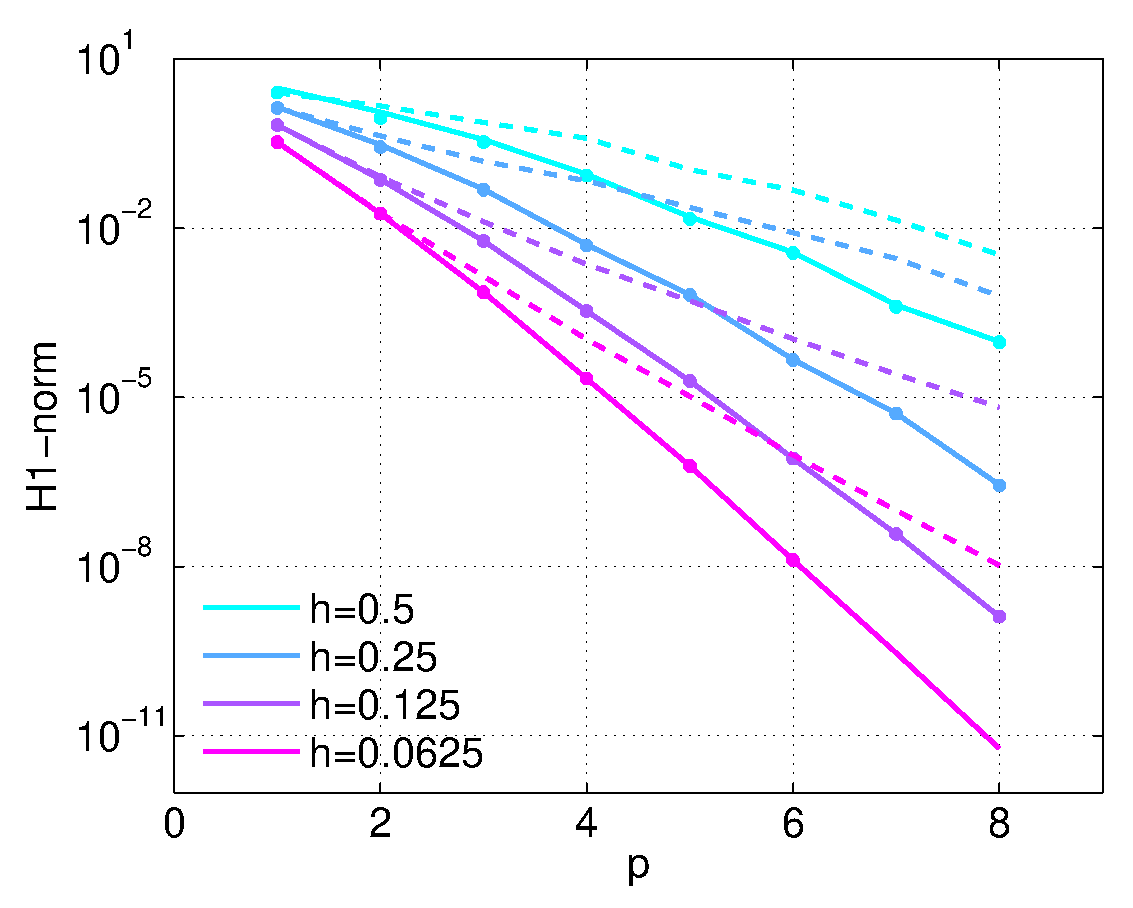
\includegraphics[width=0.48\textwidth]{Images/errH1_3d_p.eps}
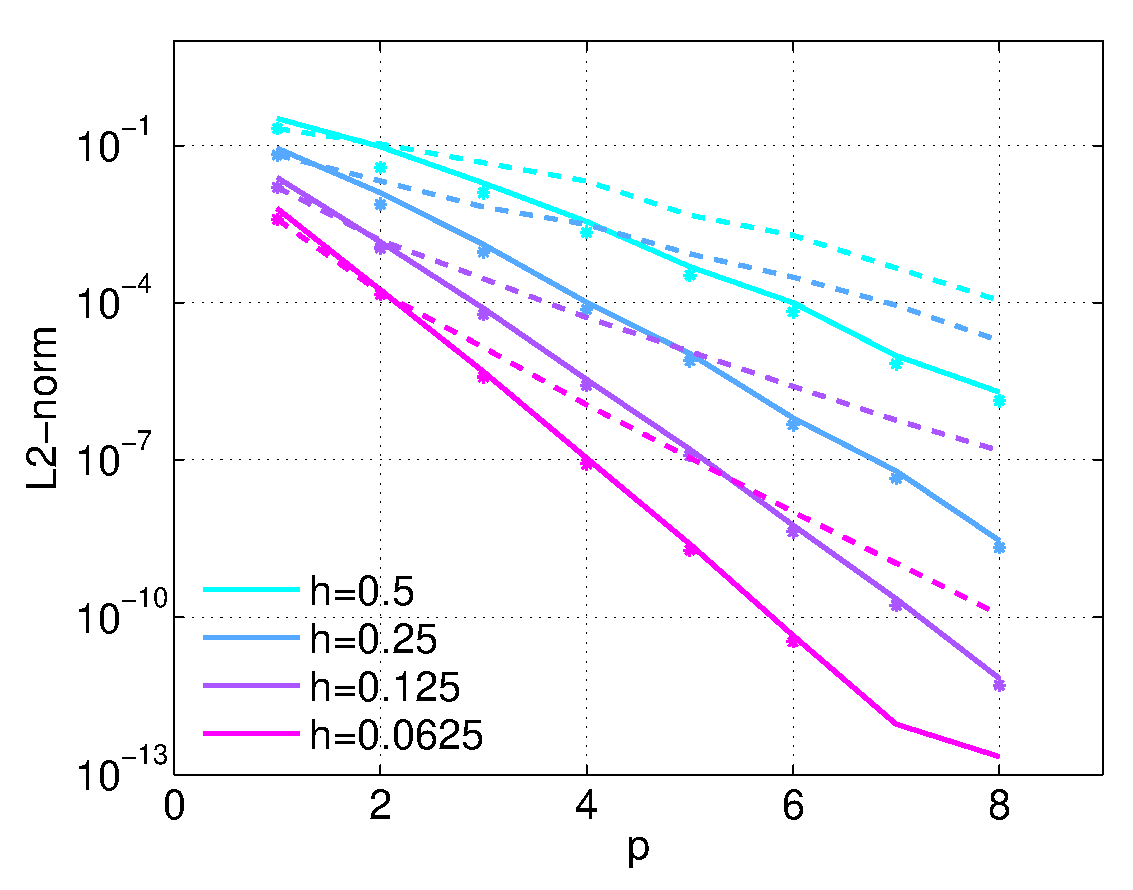
\includegraphics[width=0.48\textwidth]{Images/errL2_3d_p.eps}\\
\caption{$H^1-$norm   (left) and $L^2-$norm (right) of the errors versus 
the polynomial degree $p$. Markers refer to IGA-$C^0$ solution, 
dashed lines refer to IGA-$C^{p-1}$ solution, while the continuous lines 
refer to SEM solution. The color identifies the mesh size $h$}
\label{fig:errori_H1L2_p}
\end{figure}

% ~~~~~~~~~~~~~~~~~~~~~~~~~
% vs h
% ~~~~~~~~~~~~~~~~~~~~~~~~~~~~~
In Figure \ref{fig:errori_H1L2_h} we show the $H^1$-norm (top) and the
$L^2$-norm (bottom) of the errors between the
numerical solutions  and the exact solution
(\ref{ex_sol}), versus the mesh size $h$, when $p$ is fixed. In 
Table \ref{tab:ordini_h} we show the convergence orders w.r.t. $h$, that we have
estimated starting from the errors reported in Fig. \ref{fig:errori_H1L2_h}.
The errors of IGA-$C^0$ and SEM obey the estimates (\ref{stima_sem}) and (\ref{stima_h_iga})
with respect to $h$, while the errors of IGA-$C^{p-1}$ exhibit
superconvergence w.r.t. $h$.


\begin{figure}
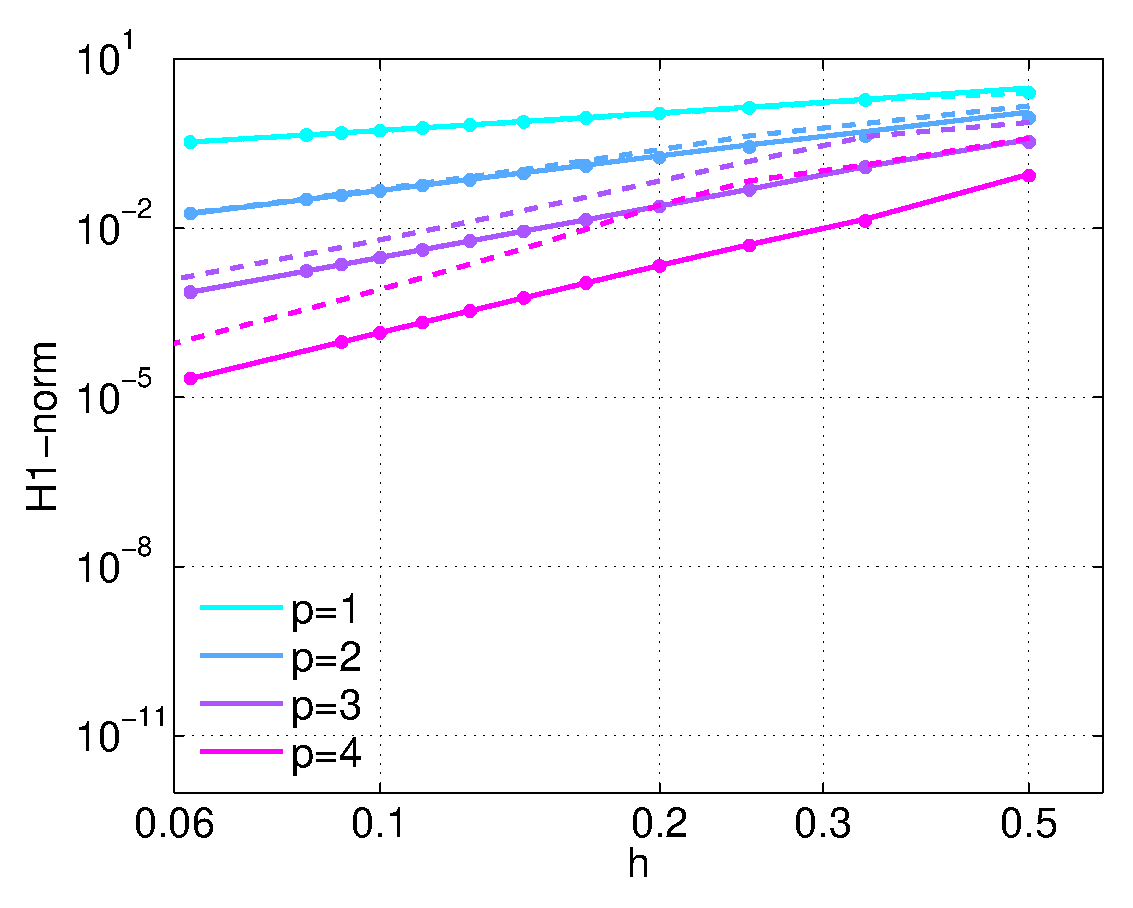
\includegraphics[width=0.48\textwidth]{Images/errH1_3d_ha.eps}
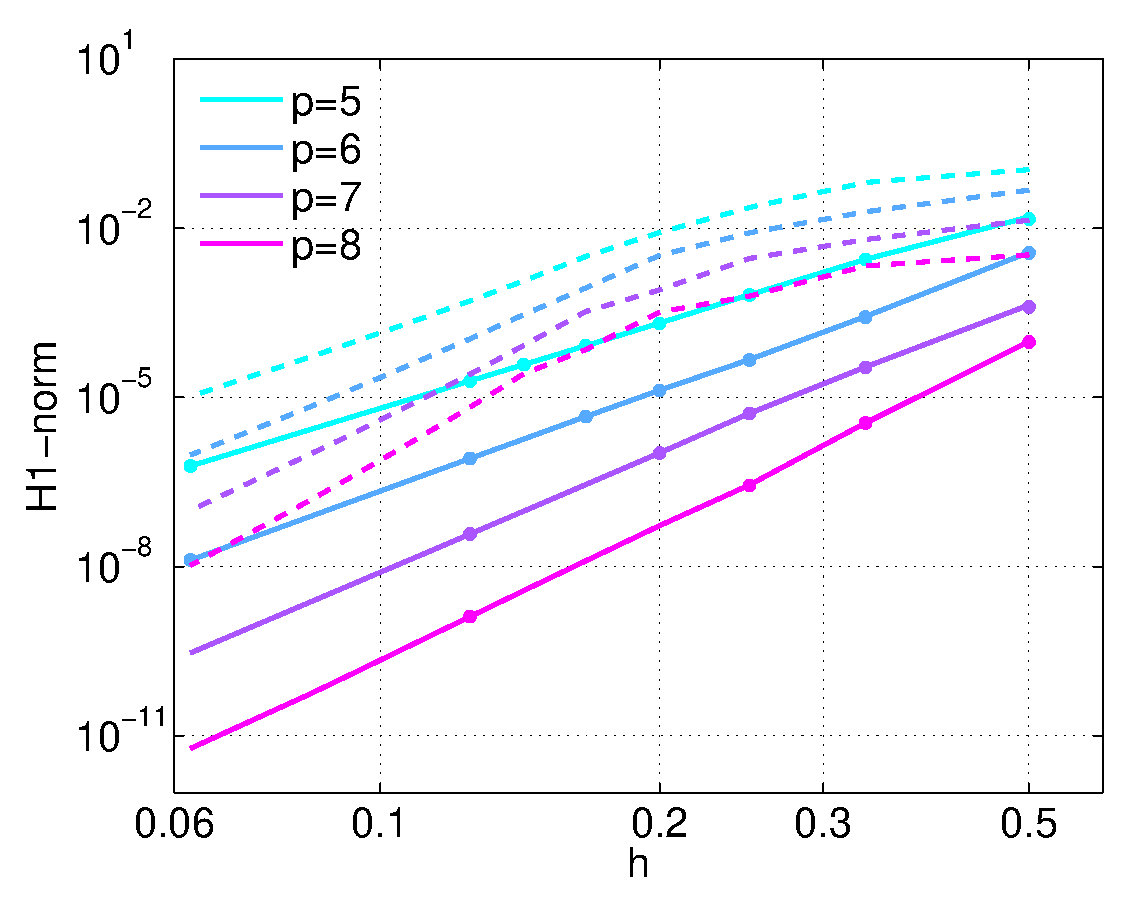
\includegraphics[width=0.48\textwidth]{Images/errH1_3d_hb.eps}\\
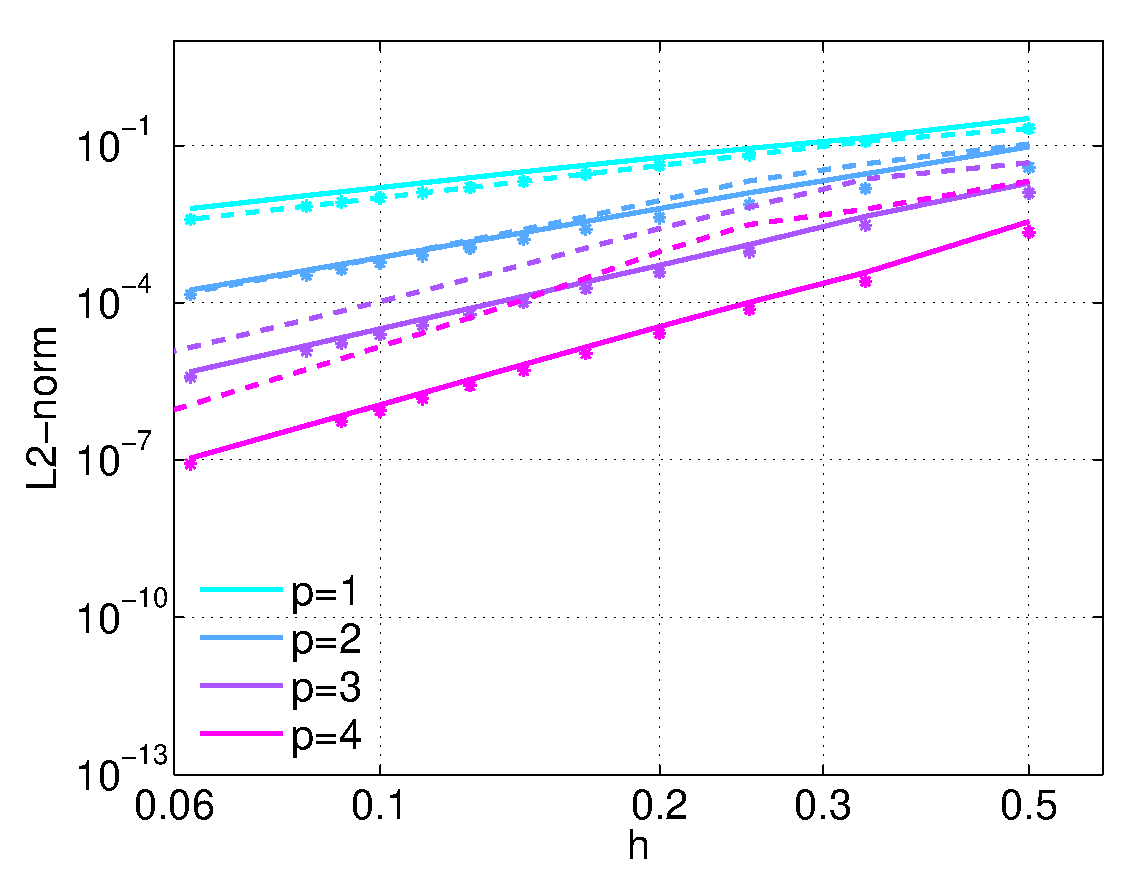
\includegraphics[width=0.48\textwidth]{Images/errL2_3d_ha.eps}
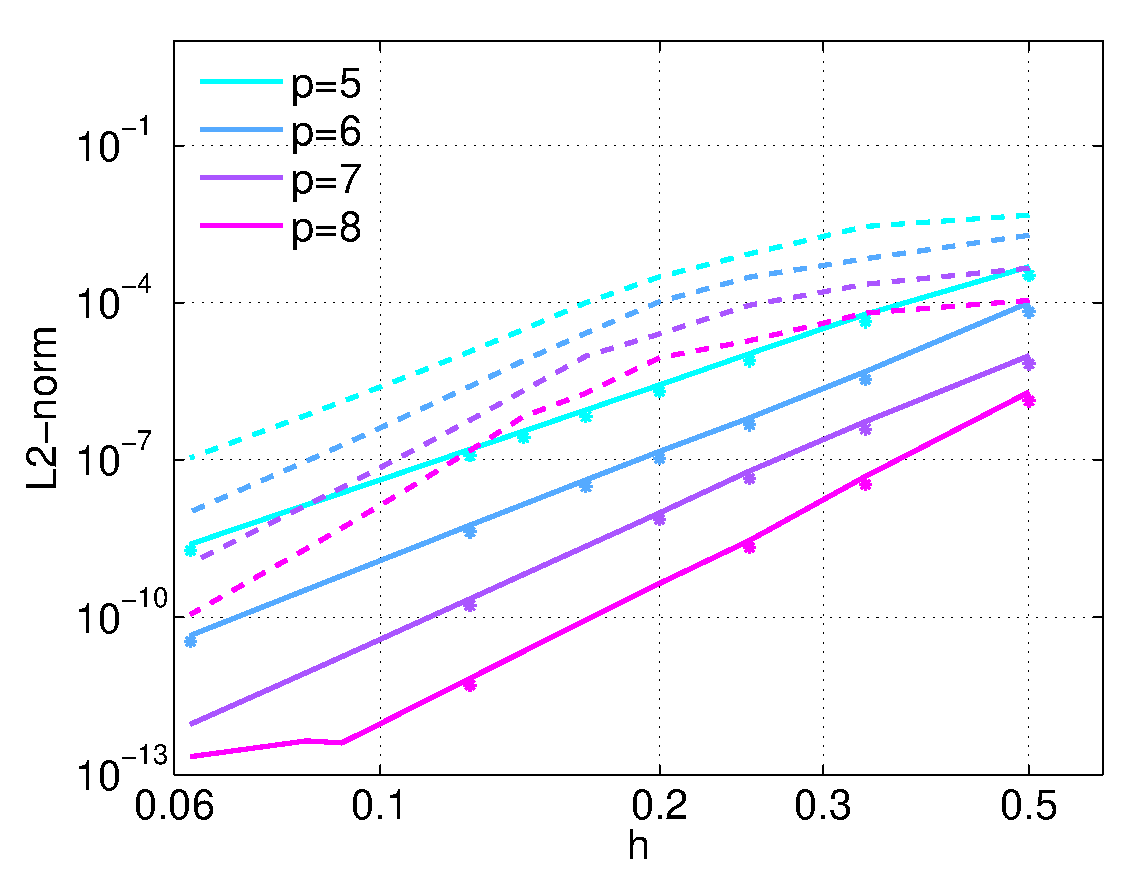
\includegraphics[width=0.48\textwidth]{Images/errL2_3d_hb.eps}\\
\caption{$H^1-$norm   (top) and $L^2-$norm (bottom) of the errors 
versus the mesh size $h$.
Markers refer to IGA-$C^0$ solution, dashed lines refer to IGA-$C^{p-1}$
solution, while continuous lines refer to SEM solution. The color identifies the
polynomial degree $p$}
\label{fig:errori_H1L2_h}
\end{figure}


\begin{table}
\caption{Convergence orders w.r.t. $h$}\label{tab:ordini_h}
\begin{center}
\begin{tabular}{c|ccc|ccc}
& \multicolumn{3}{c|}{$H^1-$norm}&\multicolumn{3}{c}{$L^2-$norm}\\
$p$ & IGA-$C^0$ & IGA-$C^{p-1}$ & SEM& IGA-$C^0$ & IGA-$C^{p-1}$ & SEM\\
\hline
1 & 1.00 & 1.00 & 1.02 & 2.02 & 2.02 & 1.95 \\
2 & 1.99 & 2.15 & 2.02 & 2.94 & 3.35 & 3.06 \\ 
3 & 3.00 & 3.08 & 3.01 & 3.97 & 4.15 & 4.01 \\
4 & 3.97 & 4.16 & 3.99 & 4.95 & 5.23 & 4.99\\
5 & 5.03 & 5.70 & 5.01 & 6.00 & 6.82 & 6.00\\
6 & 5.99 & 6.93 & 5.98 & 6.93 & 8.05 & 6.98 \\
7 & 6.71 & 8.13 & 7.01 & 7.68 & 9.17 & 7.96\\
8 & 8.09 & 9.16 & 7.82 & 9.03 &10.52 & 8.92 \\
\end{tabular}
\end{center}
\end{table}


% ~~~~~~~~~~~~~~~~~~~~~~~~~
% vs dof(p)
% ~~~~~~~~~~~~~~~~~~~~~~~~~~~~~

\null
\emph{Error versus dof}

The total
number of degrees of freedom ($dof$) of the discretization
is reported below:

\begin{center}
\begin{tabular}{r|ccc}
 & IGA-$C^0$ & IGA-$C^{p-1}$ & SEM\\
\hline\\[-2mm]
$dof $ & $(np+1)^d$ & $(p+n)^d$ & $(np+1)^d$.
\end{tabular}
\end{center}

In Figure \ref{fig:errori_H1L2_dofp} the $H^1$-norm (at left) and the
$L^2$-norm (at right) of the errors are plotted 
versus $dof=dof(p)$, with $h$ fixed.

Similarly, in Figure \ref{fig:errori_H1L2_dofh} we report the $H^1$-norm (top) 
and the $L^2$-norm (bottom) of the errors
versus $dof=dof(h)$, with $p$ fixed.


\begin{figure}
\includegraphics[width=0.48\textwidth]{Images/errdofH1_3d_p.eps}
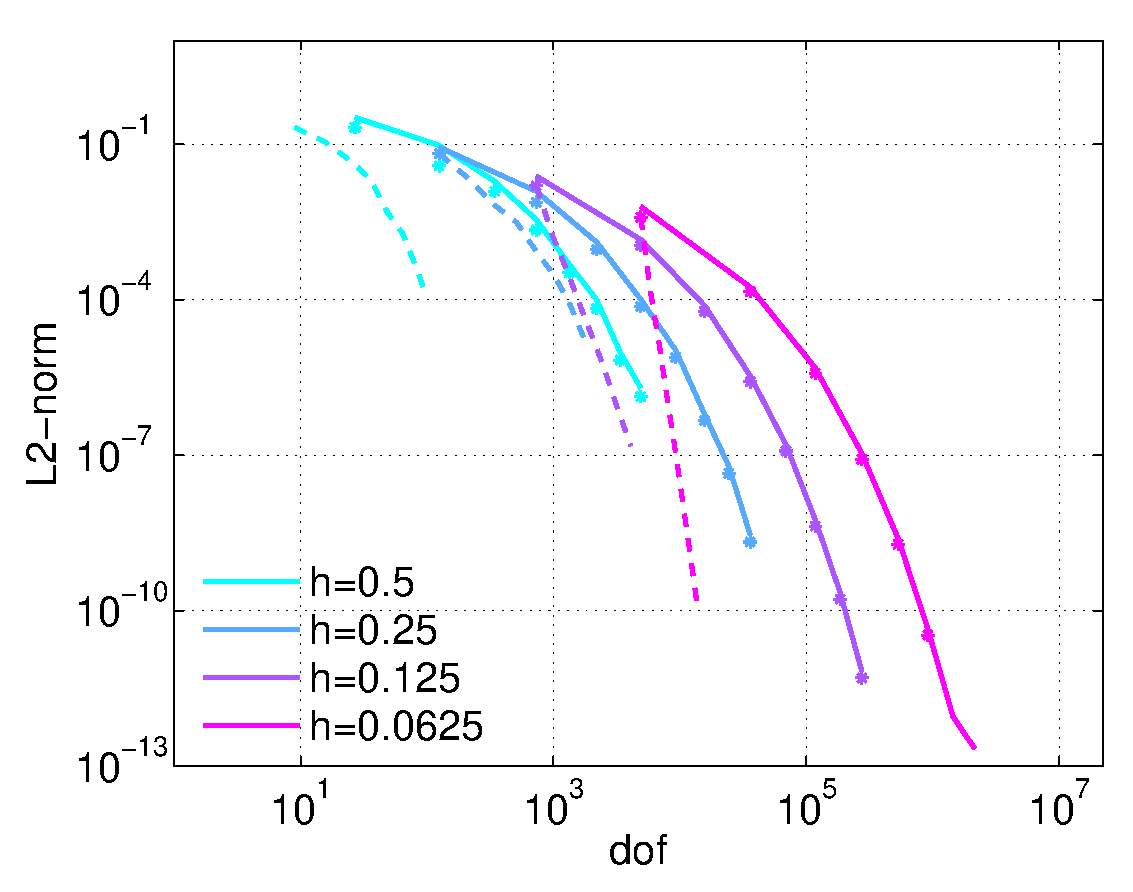
\includegraphics[width=0.48\textwidth]{Images/errdofL2_3d_p.eps}\\
\caption{$H^1-$norm   (left) and $L^2-$norm (right) of the errors versus 
$dof=dof(p)$.
Markers refer to IGA-$C^0$ solution, dashed lines refer to IGA-$C^{p-1}$
solution, while the continuous lines refer to SEM solution. 
The color identifies the
mesh size $h$}
\label{fig:errori_H1L2_dofp}
\end{figure}

\begin{figure}
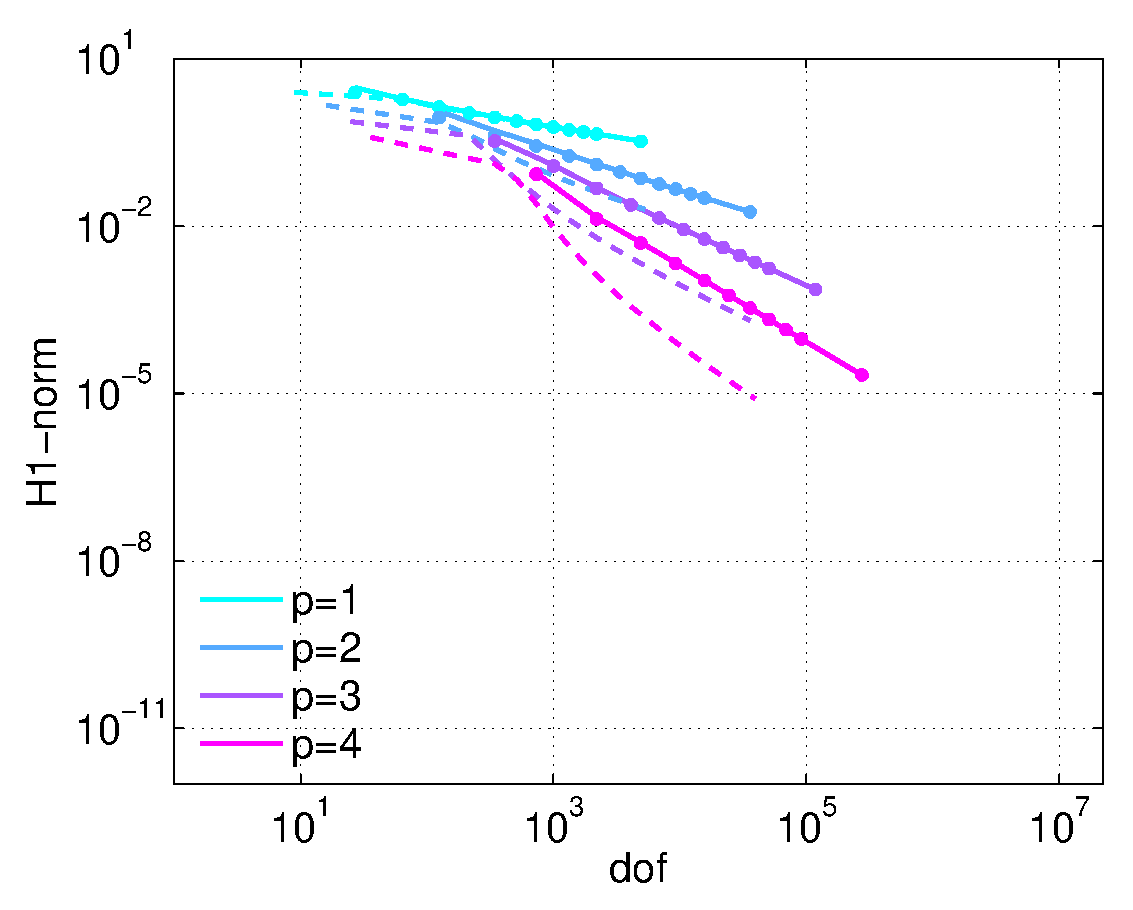
\includegraphics[width=0.48\textwidth]{Images/errdofH1_3d_ha.eps}
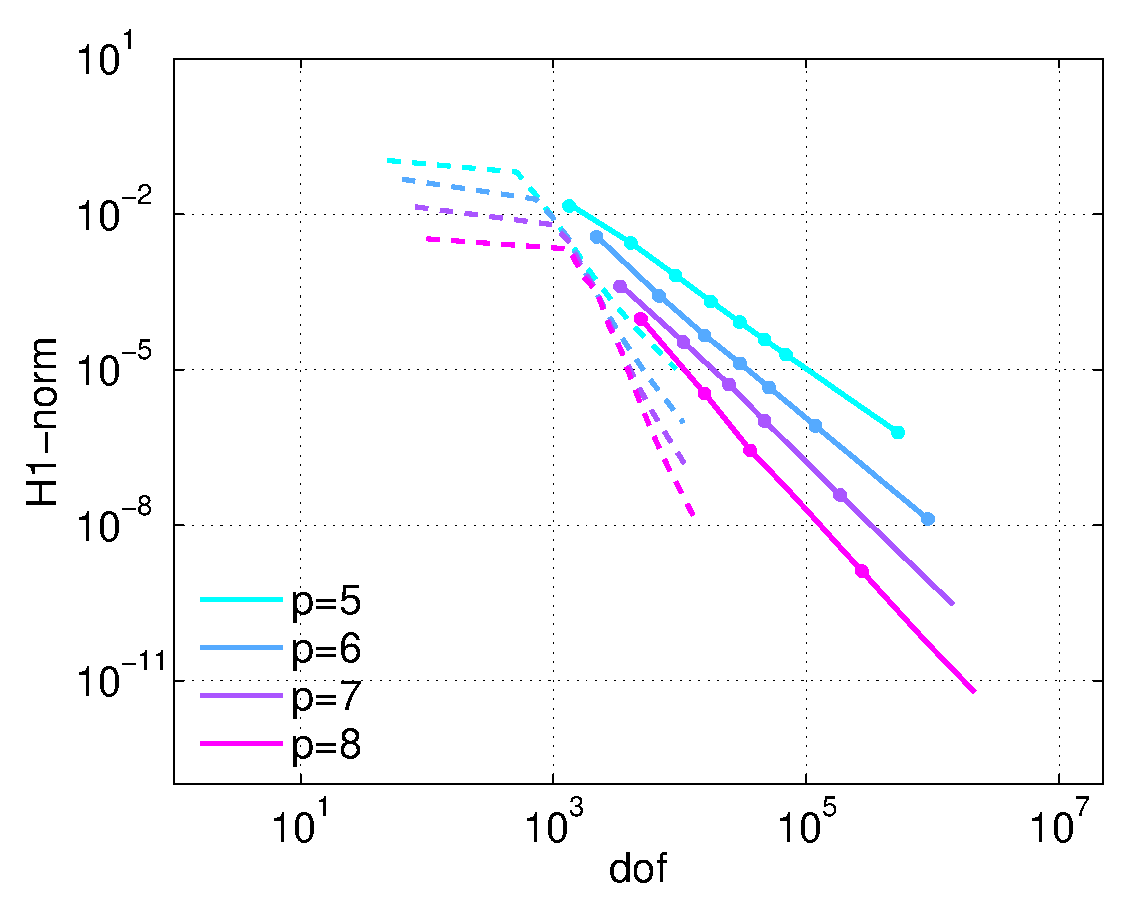
\includegraphics[width=0.48\textwidth]{Images/errdofH1_3d_hb.eps}\\
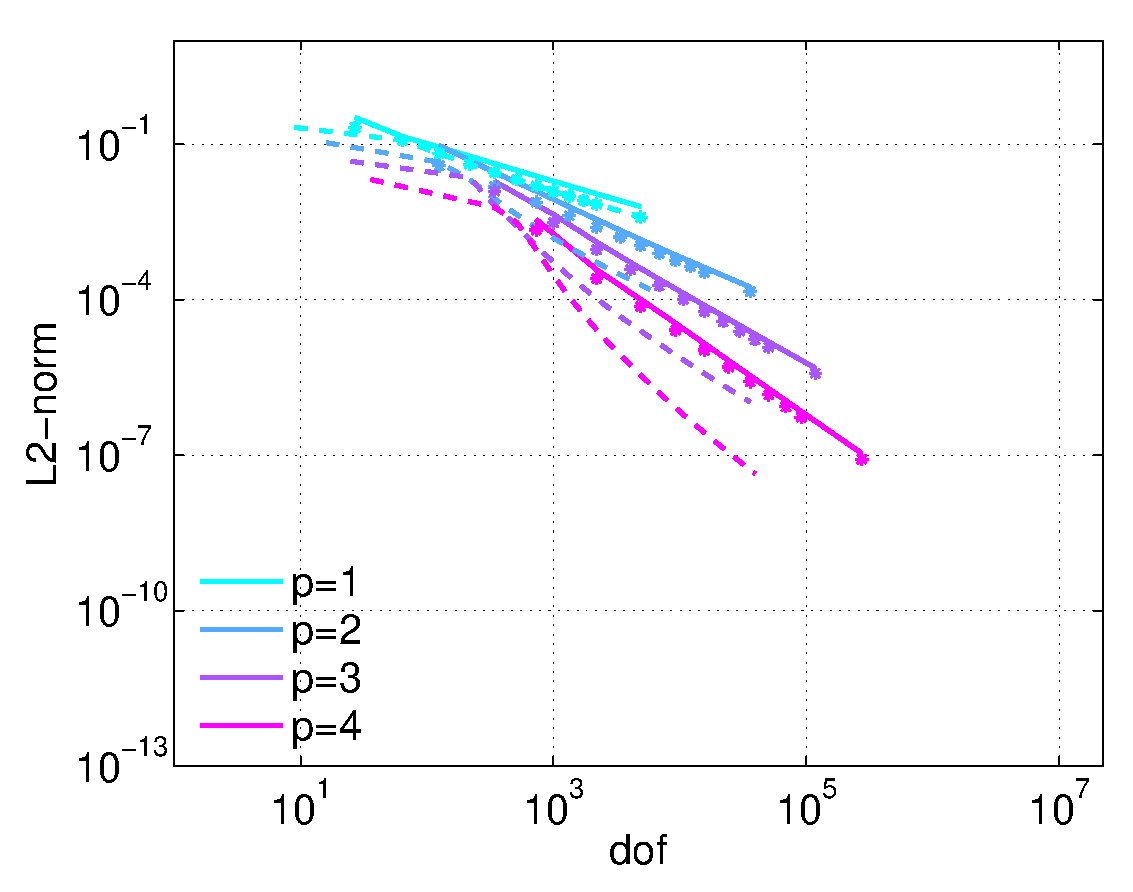
\includegraphics[width=0.48\textwidth]{Images/errdofL2_3d_ha.eps}
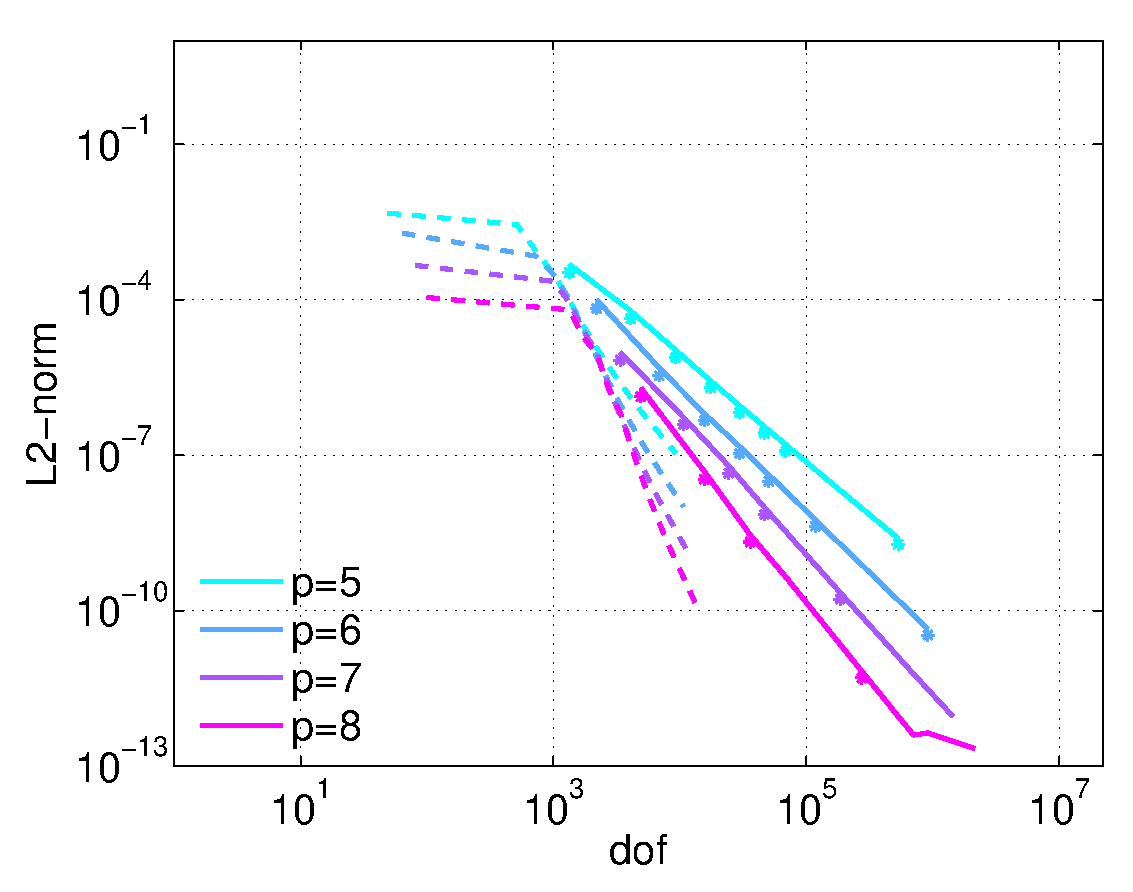
\includegraphics[width=0.48\textwidth]{Images/errdofL2_3d_hb.eps}\\
\caption{$H^1-$norm   (top) and $L^2-$norm (bottom) of the errors versus 
$dof=dof(h)$.
Markers refer to IGA-$C^0$ solution, dashed lines refer to IGA-$C^{p-1}$
solution, while the continuous lines refer to SEM solution. 
The color identifies the polynomial degree $p$}
\label{fig:errori_H1L2_dofh}
\end{figure}

IGA-$C^{p-1}$ provides the minimum error
(compared with IGA-$C^0$ and SEM) for a fixed $dof$.

\null
\emph{Matrix sparsisty pattern}

Nevertheless, $dof$ is not the unique reference parameter that we have to take 
into account in measuring the efficiency of a method.

As a matter of fact, other important ingredients that get into the game 
in solving the linear systems (\ref{algebraic_sem}) and
(\ref{algebraic_iga}), especially when $d=3$,
 are the sparsity pattern of the stiffness matrix and
its \emph{number of nonzero entries} ($nnz$).
The latter is a measure not only of the memory space
required to storage the matrix, but also of the computational 
complexity of the algebraic solver.

The numerical results shown in this Sections have been produced using an
Intel(R) Core(TM) i7-4790 CPU @ 3.60GHz with 4 Cores and 16GB  of RAM.
When $d=3$, starting from moderate values of $p$ (e.g. $p=4$) and moderate
values of $n=1/h$ (e.g. $n=8$) the direct solution of linear systems
(\ref{algebraic_sem}) and
(\ref{algebraic_iga}) is prohibitive, 
unless one has highly powerfull architectures available. 
 This is due to the fill-in occuring during 
the eliminitation  process.

As a consequence a preconditioned
 iterative method, like, e.g., Krylov ones, is in order. 
To solve the linear systems we called the Bi-GCStab method \cite{vander2003},
preconditioned by an incomplete LU factorization. 
On this machine, the iterative numerical solution of the linear 
system of IGA-$C^0$ becomes
prohibitive for $p>4$ and $n>7$. 

Even if both the  IGA and SEM
stiffness matrices are symmetric and positive definite, we have called the
Bi-GCStab instead of the Conjugate Gradient method.
As a matter of fact, since the condition
number of the IGA stiffness matrices heavily grows with $p$ (see the next
sections), the symmetric incomplete
Cholesky factorization often broke for having tried to compute the 
square root of non-positive values.


At each iteration of the Krylov method,
one has to compute matrix-vector products and solve 
auxiliary linear systems related to the preconditioner. We neglect here the
analysis of the costs associated with the preconditioner, 
that goes out the porpuses of
the present work.  

The computational costs of one matrix-vector products ($mvp$ 
in brief) is about
 $2\, nnz$ floating point operations, thus it is meaningful to measure the 
approximation errors also in terms of this parameter.

First of all we notice that $nnz$ can be written in terms of $n=1/h$ and $p$ as
($c$ is a positive constant independent of $n$ and $p$ 
that can be different method by method)
\begin{center}
\begin{tabular}{r|ccc}
 & IGA-$C^0$ & IGA-$C^{p-1}$ & SEM\\
\hline\\[-2mm]
$nnz $ & $c\,p^{2d}n^d$ & $c\,(p^{2d}+p^dn^d)$ & $c\,d\,p^{d+1}n^d$.
\end{tabular}
\end{center}

While the dependence on $n$ (and then on $h$) is the same for all the three 
methods, the dependence on $p$ strongly varies method by method.

We notice that, in the case of SEM, $nnz$ is independent of the fact that
quadrature formulas are used to approximate integrals. The same sparsity 
pattern would be obtained if one uses exact integration instead of the numerical one.

In Fig. \ref{fig:spyA} the pattern of the stiffness matrix of 
all the three methods are shown, for the case $p=4$ and $n=4$, when $d=3$.

\begin{figure}
\includegraphics[width=0.3\textwidth]{Images/matiga0_3d.pdf}
\includegraphics[width=0.3\textwidth]{Images/matigap_3d.pdf}
\includegraphics[width=0.3\textwidth]{Images/matsem_3d.pdf}
\caption{Pattern of the stiffness matrix of IGA-$C^0$ (left), IGA-$C^{p-1}$
(center), and SEM (right). $dof$ is 4193 for both IGA-$C^0$ and SEM, while it is
512 for IGA-$C^{p-1}$.
$nnz$ is 911599 for IGA-$C^0$, 
140604 for IGA-$C^{p-1}$, and 46575 for SEM}
\label{fig:spyA}
\end{figure}

Then, in Fig. \ref{fig:errori_H1L2_nnz} we show the $H^1$-norm 
of the error versus $nnz=nnz(p)$ with $h$ fixed (top) 
and  versus $nnz=nnz(h)$ with $p$ fixed (bottom).


In both cases, SEM is 
the method (among the three) that provides the minimum errors
for  $nnz$ fixed.


\begin{figure}
\begin{center}
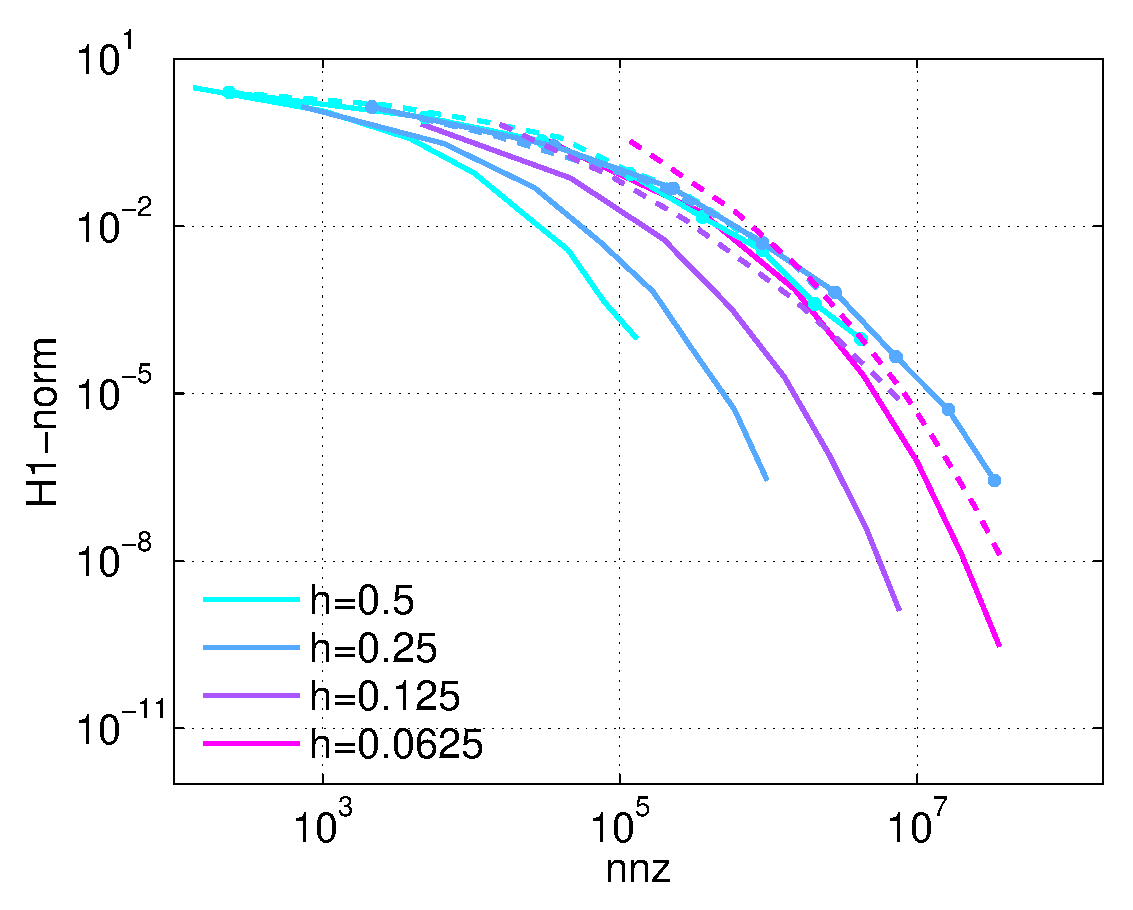
\includegraphics[width=0.48\textwidth]{Images/errnnzH1_3d_p.eps}\\
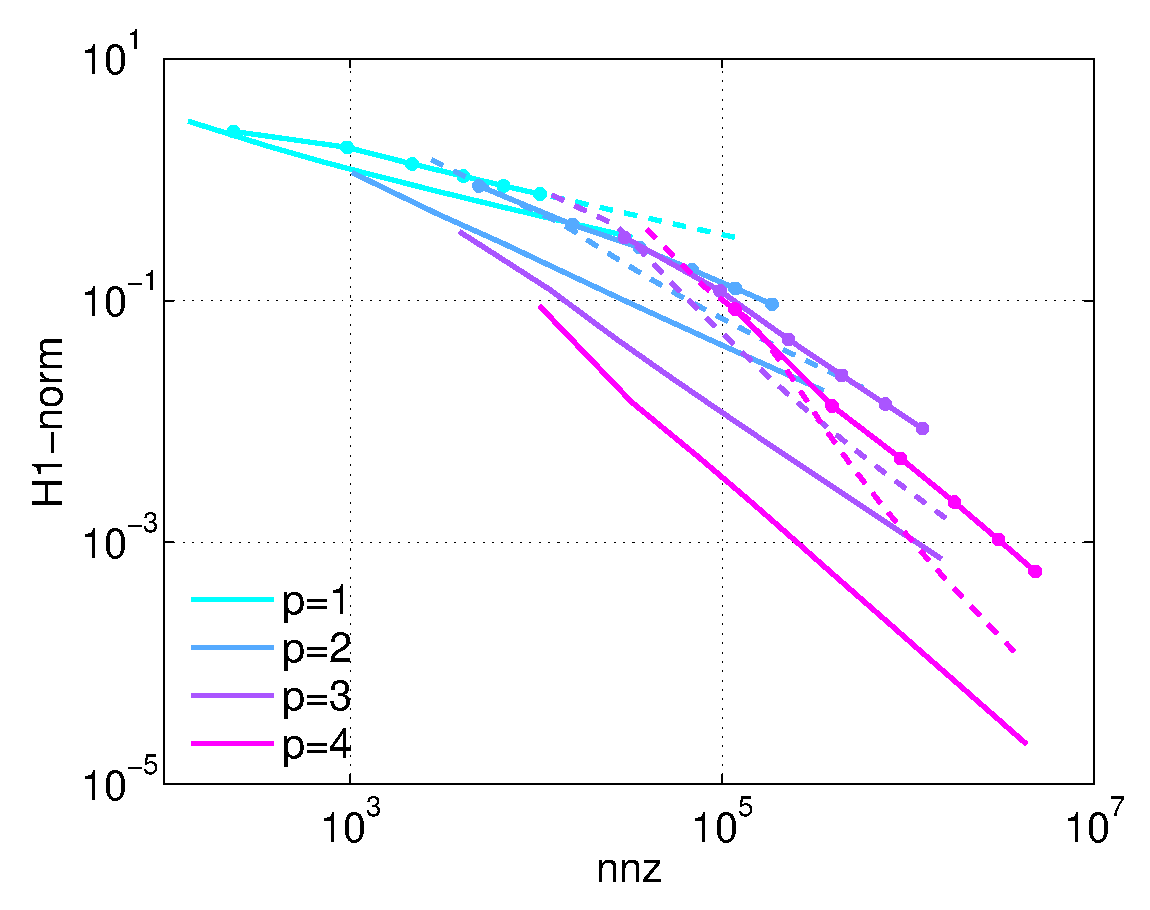
\includegraphics[width=0.48\textwidth]{Images/errnnzH1_3d_ha.eps}
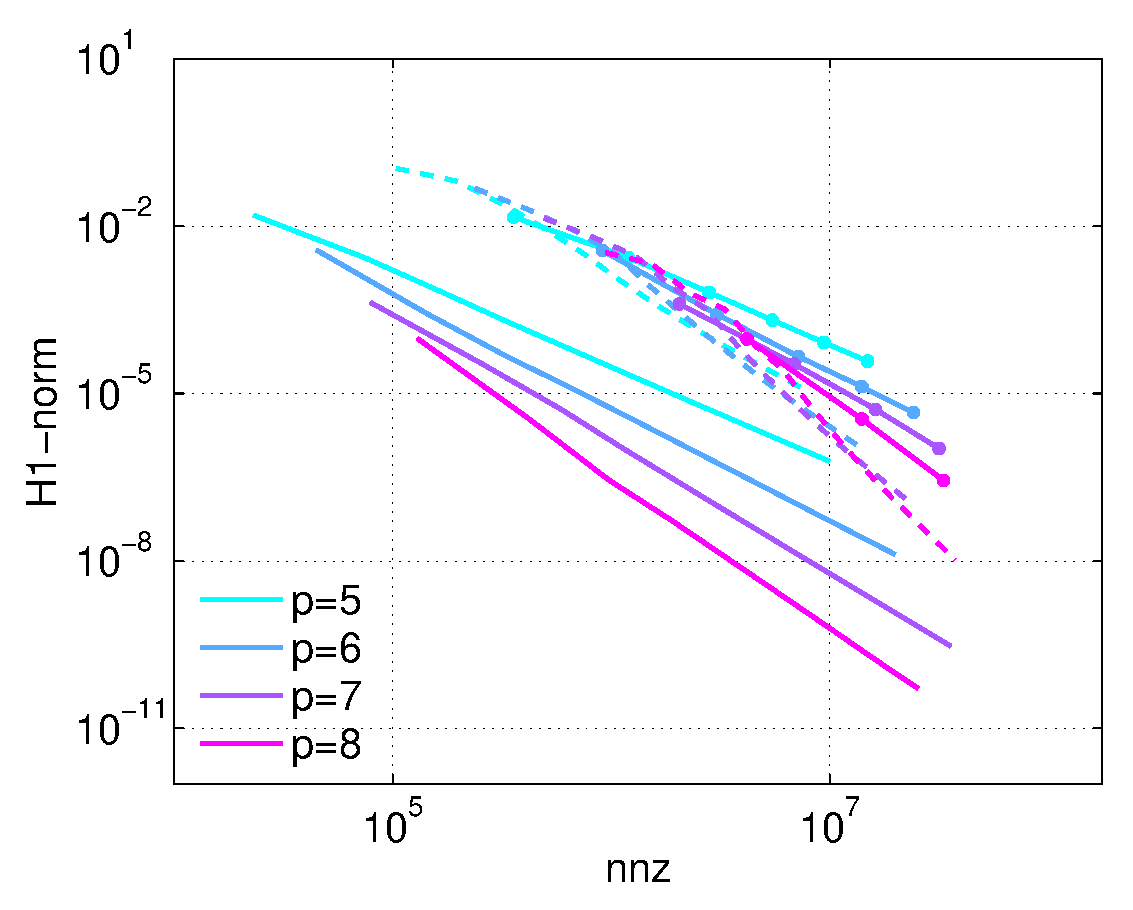
\includegraphics[width=0.48\textwidth]{Images/errnnzH1_3d_hb.eps}
\end{center}
\caption{$H^1-$norm of the error versus
$nnz=nnz(p)$ (top) and versus
$nnz=nnz(h)$ (bottom).
Markers refer to IGA-$C^0$ solution, dashed lines refer to IGA-$C^{p-1}$
solution, while the continuous lines refer to SEM solution.
The color identifies the
mesh size $h$}
\label{fig:errori_H1L2_nnz}
\end{figure}

%{\pg Io non riporterei i tempi di CPU in quanto 
%dipendono fortemente dal precondizionatore
%che si usa ed e' un lavoro lunghissimo tarare il precondizionatore giusto per
%ogni metodo.
%Al momento ho usato incomplete LU factorization di matlab.
%
%
%Per IGA-C0 non riesco a costruire un precondizionatore che stia in memoria
%(16GB di ram) e che dia convergenza per $p>4$ e $h<1/7$.
%
%Per IGA-$C^{p-1}$ sono riuscita a far andare il codice con $p<=8$ e $h<=16$
%mettendo drop-tolerance =$10^{-7}$ (quindi precondizionatore molto pieno).
%
%Per SEM sono riuscita a far andare il codice con $p<=8$ e $h<=16$
%mettendo drop-tolerance =$10^{-3}$.
%
%I costi dei precondizionatori sono molto molto diversi.}



%\clearpage
%\newpage
%-------------------------------------------
%  Eigenvalues
% -------------------------------------------
\section{Extreme eigenvalues and condition number}

{\aq In this section we summarize the main results concerning the spectral
properties of SEM and IGA arrays. Because of their importance for the 
convergence rate of iterative methods, we specifically highlight the 
behaviour of the extreme eigenvalues (and the corresponding spectral
condition number) of mass matrices and stiffness matrices.}

%Preconditioners are proposed in \cite{sangalli_tani_sisc,pavarino_scacchi,bcps,
%bpswz_2017,bpswz_2014,bcps13a,bpcs13b}

\null
For any matrix $A$ symmetric positive definite (or similar to 
a symmetric positive definite matrix)
let $\lambda_{min}(A)$  and 
$\lambda_{max}(A)$ denote its minimum and maximum (real) eigenvalues,
respectively.
The \emph{spectral condition number} of $A$ is defined as
\begin{equation}\label{iter_cond}
{\cal K}(A)=\frac{\lambda_{max}(A)}{\lambda_{min}(A)}.
\end{equation}

%In Table \ref{tab:cond} we summarize the behaviour of the spectral condition
%numbers of eithar mass and stiffness matrices.
 
\begin{table}
\caption{Condition numbers of mass and stiffness matrices}
\label{tab:cond}
\begin{tabular}{|>{\centering}m{0.06\textwidth}| >{\centering}m{0.06\textwidth}|
>{\centering}m{0.38\textwidth}| >{\centering\arraybackslash}m{0.38\textwidth}|}
\hline
& SEM & IGA-$C^0$ & IGA-$C^{p-1}$\\
\hline
{${\cal K}(M)$} &
{$p^d$} &
{$p^{-d/2}4^{pd}$} &
\scalebox{0.4}{\input{mass_cond_igap.pdf_t}}\\
\hline
{${\cal K}(K)$} &
{$h^{-2}p^3$} &
\scalebox{0.4}{\input{stiff_cond_iga0.pdf_t}}&
\scalebox{0.4}{\input{stiff_cond_igap.pdf_t}}\\
\hline
\end{tabular}
\end{table}

The extreme eigenvalues of the
SEM mass and stiffness matrices behave as follows (\cite{bm,melenk02,
chqz06,chqz07}):
\begin{eqnarray}
\label{eigminiM_sem}
\lambda_{min}(M_{SEM})&\sim& c_1 h^dp^{-2d} \\
\label{eigmaxM_sem}
\lambda_{max}(M_{SEM})&\sim& c_2 h^d p^{-d}\\
\label{eigminK_sem}
\lambda_{min}(K_{SEM})&\sim& c_3(d) h^d p^{-d}\\
\label{eigmaxK_sem}
\lambda_{max}(K_{SEM})&\sim& c_4(d) h^{d-2} p^{3-d}\\
\label{eigmingen_sem}
\lambda_{min}((M_{SEM})^{-1}K_{SEM})&\sim& c_5(d)\\
\label{eigmaxgen_sem}
\lambda_{min}((M_{SEM})^{-1}K_{SEM})&\sim& c_6(d) h^{-2}p^{4}.
\end{eqnarray}
The corresponding iterative condition numbers are, for $d=1,2,3$:
\begin{eqnarray}
\label{condM_sem}
{\cal K}(M_{SEM})&\sim& p^{d}\\
\label{condK_sem}
{\cal K}(K_{SEM})&\sim&  p^{3} h^{-2}\\
\label{condgen_sem}
{\cal K}((M_{SEM})^{-1}K_{SEM})&\sim&  p^{4} h^{-2},
\end{eqnarray}
they are reported in  Table \ref{tab:cond}.

{\pg Discorso generale sulle costanti: le lasciamo, le togliamo? Mettiamo una 
$c$ generica per tutti, altrimenti sono veramente tante.}


The eigenvalues and the condition number of IGA matrices have been studied 
in \cite{Gahalaut_Tomar,gmpscs}. 

In \cite{Gahalaut_Tomar} it is proved for $d=2$ that, independently of the
$k$-regularity of the B-spline basis functions, it holds:
\begin{eqnarray}\label{stime_GT}
\begin{array}{l}
\lambda_{min}(M_{k})\sim c(p) h^2, \qquad 
\lambda_{min}(M_{k})\geq c(h) p^{-4}16^{-p}\\[1mm]
\lambda_{max}(M_{k})\sim c(p) h^2,\qquad
\lambda_{max}(M_{k})\sim c(h)p^{-2},\\[1mm]
{\cal K}(M_{k})\leq c p^{2} 16^{p},\mbox{ with $c$ indep. of $h$ and $p$},\\[2mm]
\lambda_{min}(K_{k})\sim c(p)h^2,\\ [1mm]
\lambda_{max}(K_{k})\sim c, \mbox{ with $c$ indep. of $h$ and $p$},\\[1mm]
{\cal K}(K_{k})\leq c(h) p^{8} 16^{p},
\end{array}
\end{eqnarray}
 where $M_{k}$ and $K_{k}$ are the mass matrix and the stiffness matrix
of IGA approximation for a generic $k=0,\ldots,p-1$.

In \cite{gmpscs} the authors prove for $d=1$, $p\geq 1$ and $n\geq 2$ that
\begin{eqnarray}\label{stime_gmpscs}
\begin{array}{l}
\lambda_{min}(M_{p-1})\geq h c(p),\\
\lambda_{min}(K_{p-1})\geq \pi^2 h c(p).
\end{array}
\end{eqnarray}
Other estimates about the clustering of the 
eigenvalues of the matrix discretizing the advection-diffusion-reaction
operator for $d=1$ are proved in \cite{gmpscs}.



\null
We have numerically computed the extreme eigenvalues of the mass and 
stiffness matrices for both IGA-$C^0$ and IGA-$C^{p-1}$ using the function 
{\tt eigs} of Matlab for different values
of $h$ and $p$, then we have estimated their behaviour w.r.t. both $h$ and $p$.


%\clearpage
%\newpage
% ~~~~~~~~~~~~~~~~~~~~~~~~~~~~~~~~~
%  IGA-C0 mass
% ~~~~~~~~~~~~~~~~~~~~~~~~~~~~~~~~~
\subsection{IGA-$C^0$ mass matrix}

If we denote with $M_0$ the mass matrix associated with IGA-$C^0$ approximation,
our numerical results show that, for any value of $h>0$ and $p\geq 1$,
 $\lambda_{min}(M_0)$ and
$\lambda_{max}(M_0)$
behave as:
\begin{eqnarray}
\label{eigminM_C0}
\lambda_{min}(M_0)&\sim &c(d) h^dp^{-d/2}4^{-pd},\\
\label{eigmaxM_C0}
\lambda_{max}(M_0)& \sim &\displaystyle\frac{1}{c(d)}h^dp^{-d},
\end{eqnarray}
for $d=1,2,3$. The constants $c(d)>1$ are of the order of
the unity: $c(1)\sim 1.2$, $c(2)\sim 1.2$ and $c(3)\sim 1.7$.
Then
\begin{equation}\label{condM_C0}
{\cal K}(M_0)\sim p^{-d/2} 4^{pd}.
\end{equation}


%\begin{figure}
%\begin{center}
%\scalebox{0.5}{\input{massa_iga0.pdf_t}}\quad
%\end{center}
%\caption{Behaviour of the extreme eigenvalues of the 
%mass matrix $M_0$ of IGA-$C^0$}
%\label{fig:massa-iga0}
%\end{figure}

In Figures \ref{fig:massamin-iga0d1} -- \ref{fig:massamax-iga0d3} we 
show
the computed eigenvalues (at left) and the r.h.s. of
(\ref{eigminM_C0}) -- 
(\ref{eigmaxM_C0}) w.r.t. $h$ and $p$.

{\pg Va bene cos\`\i? Vi sembrano chiare tutte queste figure sugli autovalori? 
Pensate sia meglio 
un altro tipo di grafica?}

\begin{figure}[h]
\begin{center}
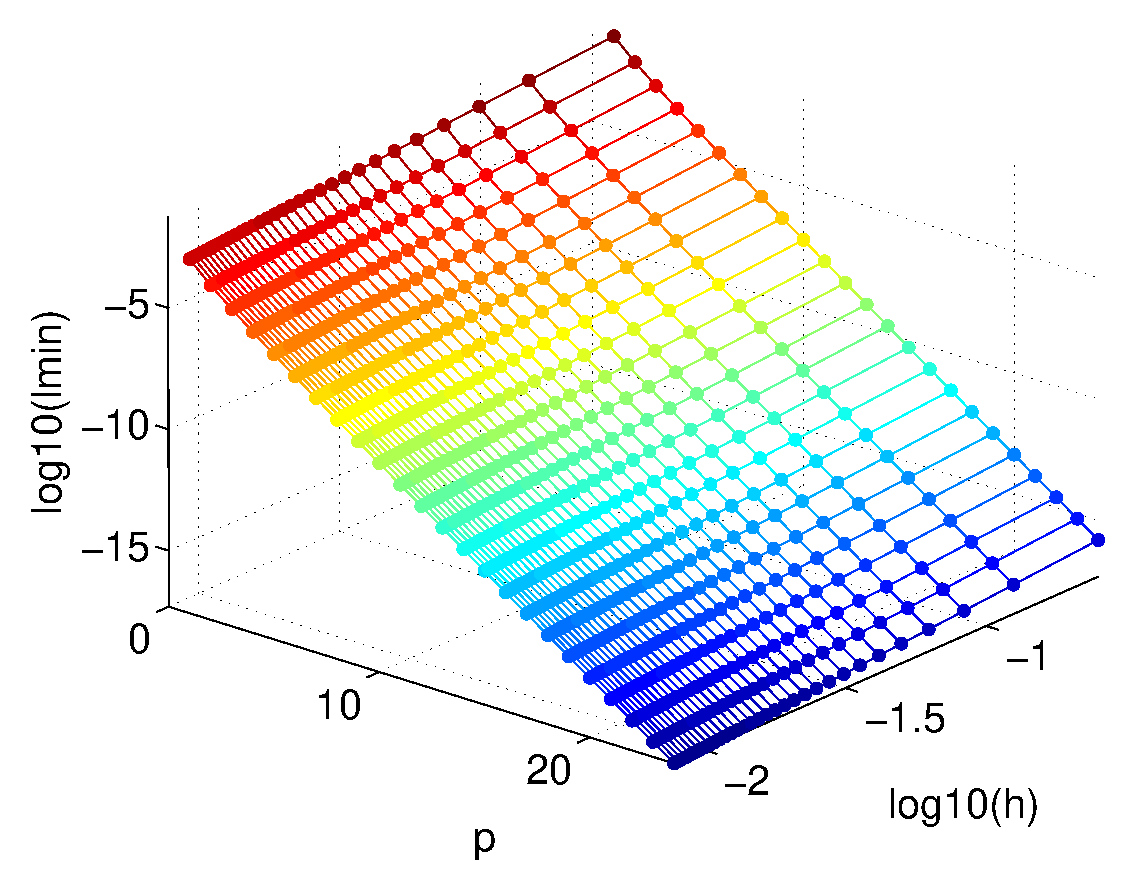
\includegraphics[width=0.45\textwidth]{Images/iga0_eigM1min.eps}\quad
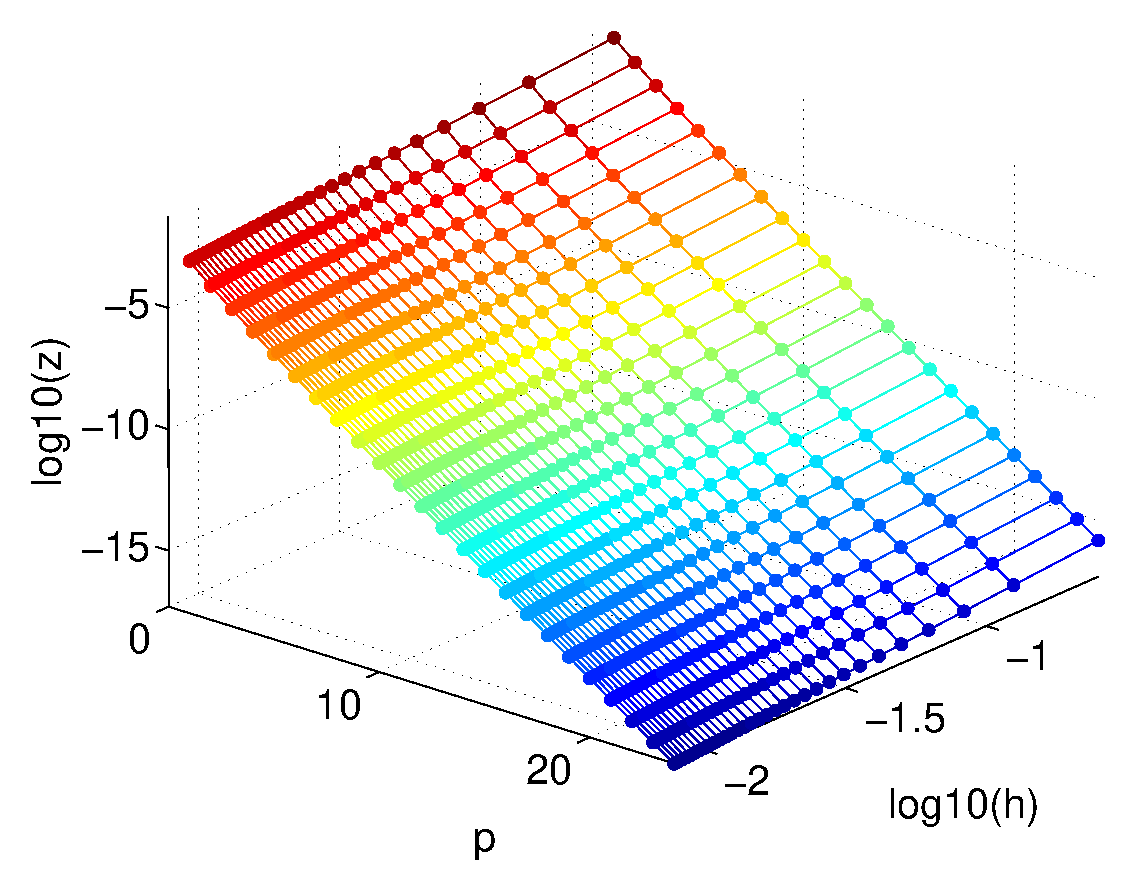
\includegraphics[width=0.45\textwidth]{Images/iga0_eigM1smin.eps}\\
\end{center}
\caption{At left, the numerically computed values of 
$\lambda_{min}(M_0)$ for $d=1$ and 
for different values of $h$ and $p$. At right, 
the graphical representation of the r.h.s. of (\ref{eigminM_C0}). $c(1)
\simeq 1.2$}
\label{fig:massamin-iga0d1}
\end{figure}


\begin{figure}[h]
\begin{center}
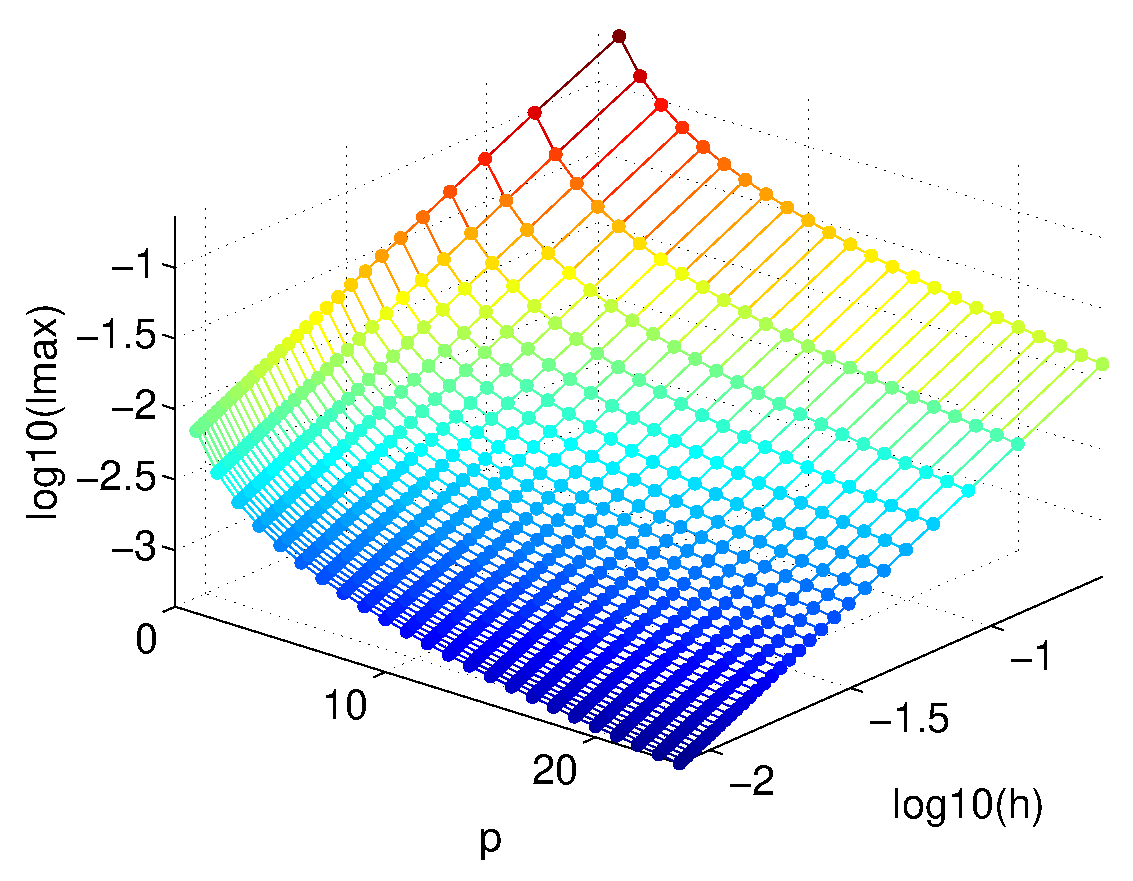
\includegraphics[width=0.45\textwidth]{Images/iga0_eigM1max.eps}\quad
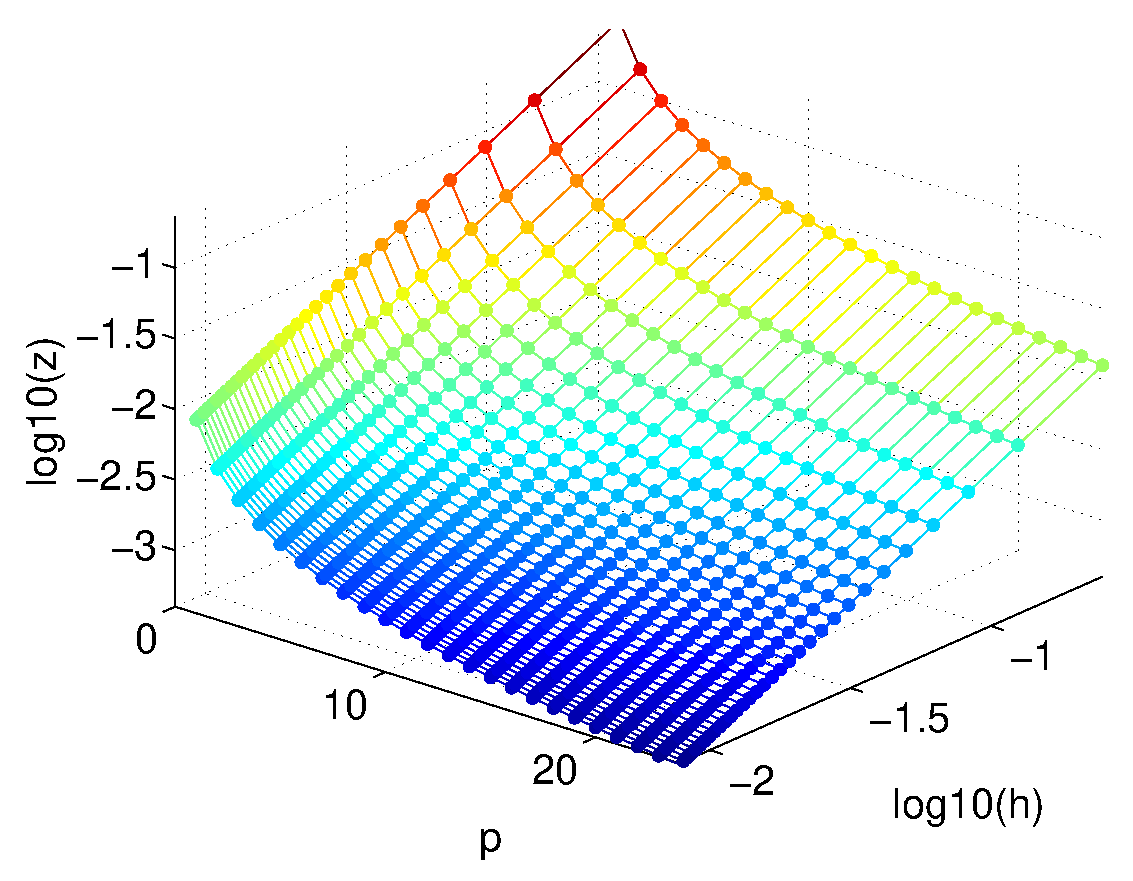
\includegraphics[width=0.45\textwidth]{Images/iga0_eigM1smax.eps}\\
\end{center}
\caption{At left, the numerically computed values of 
$\lambda_{max}(M_0)$ for $d=1$ and 
for different values of $h$ and $p$. At right, 
the graphical representation of the r.h.s. of (\ref{eigmaxM_C0}). $c(1)
\simeq 1.2$}
\label{fig:massamax-iga0d1}
\end{figure}

%\newpage
\begin{figure}
\begin{center}
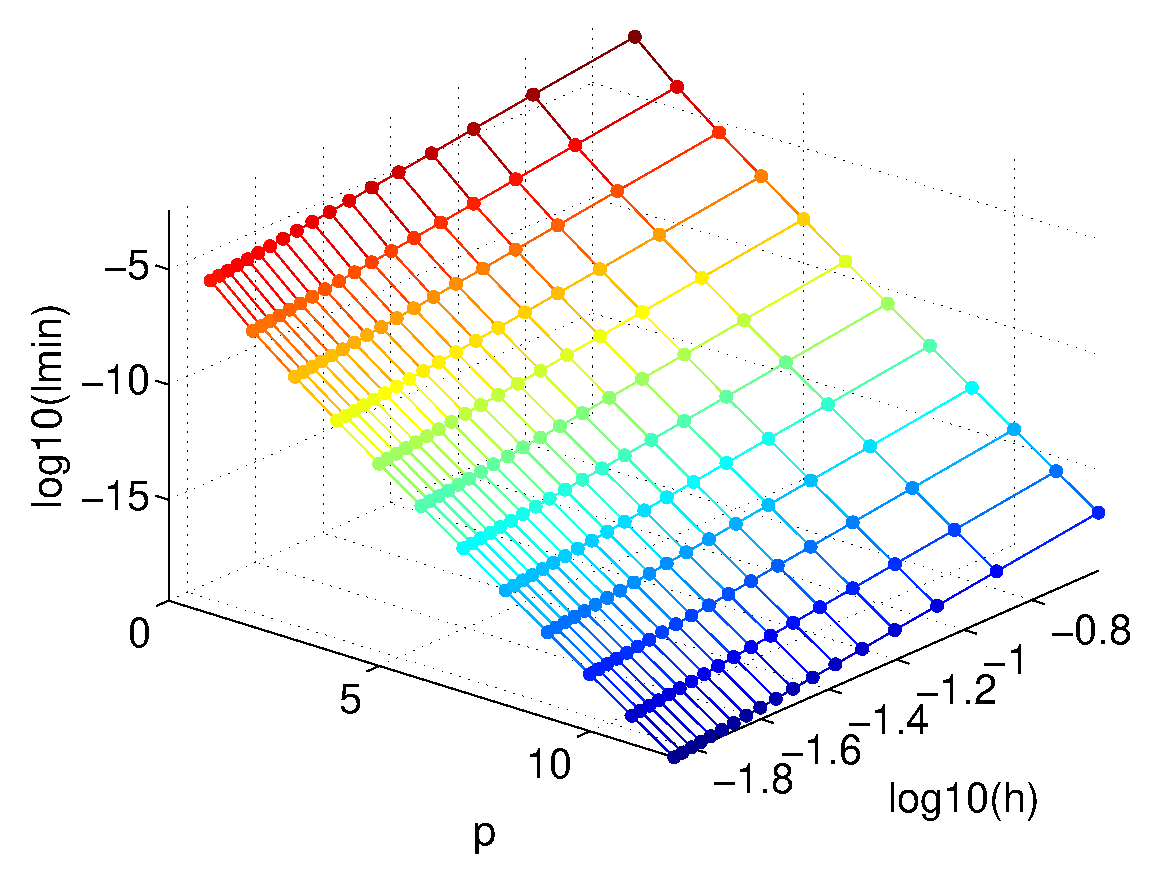
\includegraphics[width=0.45\textwidth]{Images/iga0_eigM2min.eps}\quad
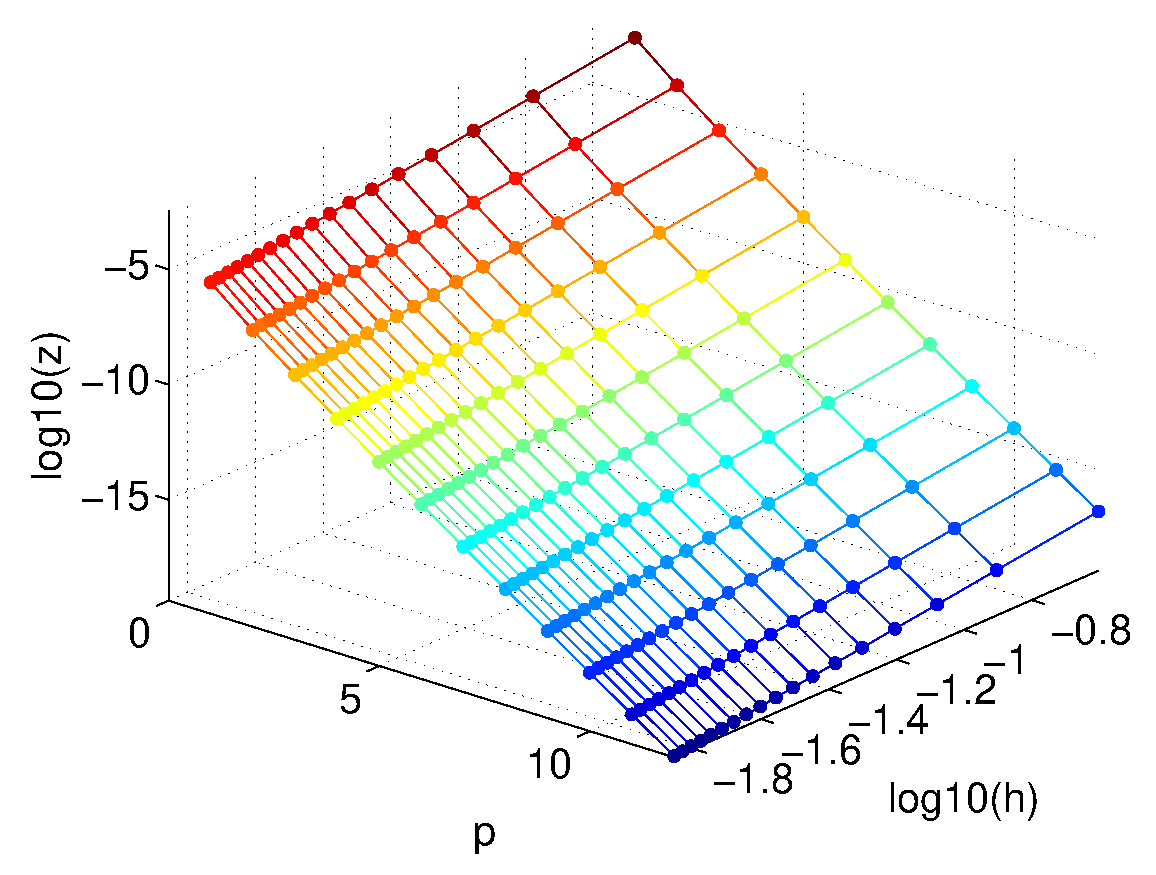
\includegraphics[width=0.45\textwidth]{Images/iga0_eigM2smin.eps}\\
\end{center}
\caption{At left, the numerically computed values of
$\lambda_{min}(M_0)$ for $d=2$ and
for different values of $h$ and $p$. At right,
the graphical representation of the r.h.s. of (\ref{eigminM_C0}). $c(2)
\simeq 1.2$}
\label{fig:massamin-iga0d2}
\end{figure}



\begin{figure}
\begin{center}
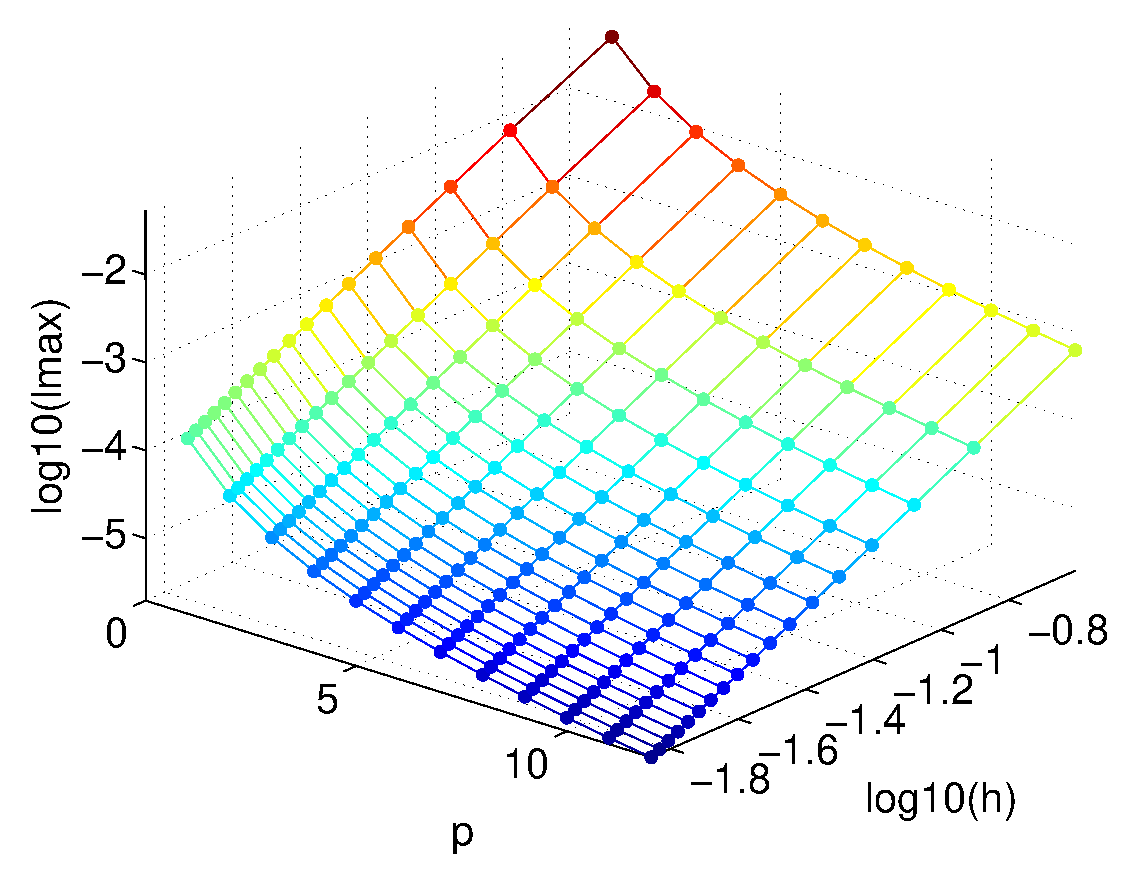
\includegraphics[width=0.45\textwidth]{Images/iga0_eigM2max.eps}\quad
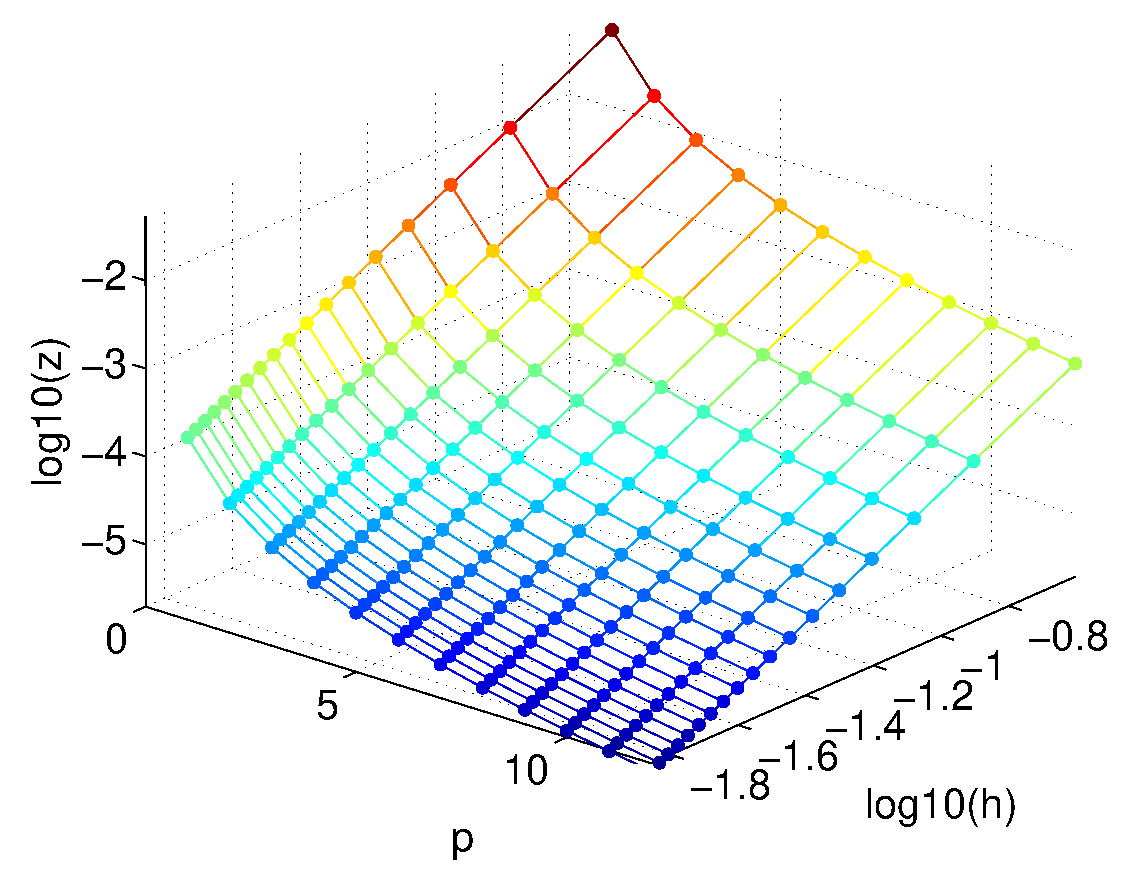
\includegraphics[width=0.45\textwidth]{Images/iga0_eigM2smax.eps}\\
\end{center}
\caption{At left, the numerically computed values of
$\lambda_{max}(M_0)$ for $d=2$ and
for different values of $h$ and $p$. At right,
the graphical representation of the r.h.s. of (\ref{eigmaxM_C0}). $c(2)
\simeq 1.2$}
\label{fig:massamax-iga0d2}
\end{figure}

%\clearpage
%\newpage
\begin{figure}
\begin{center}
\includegraphics[width=0.45\textwidth]{Images/iga0_eigM3min.eps}\quad
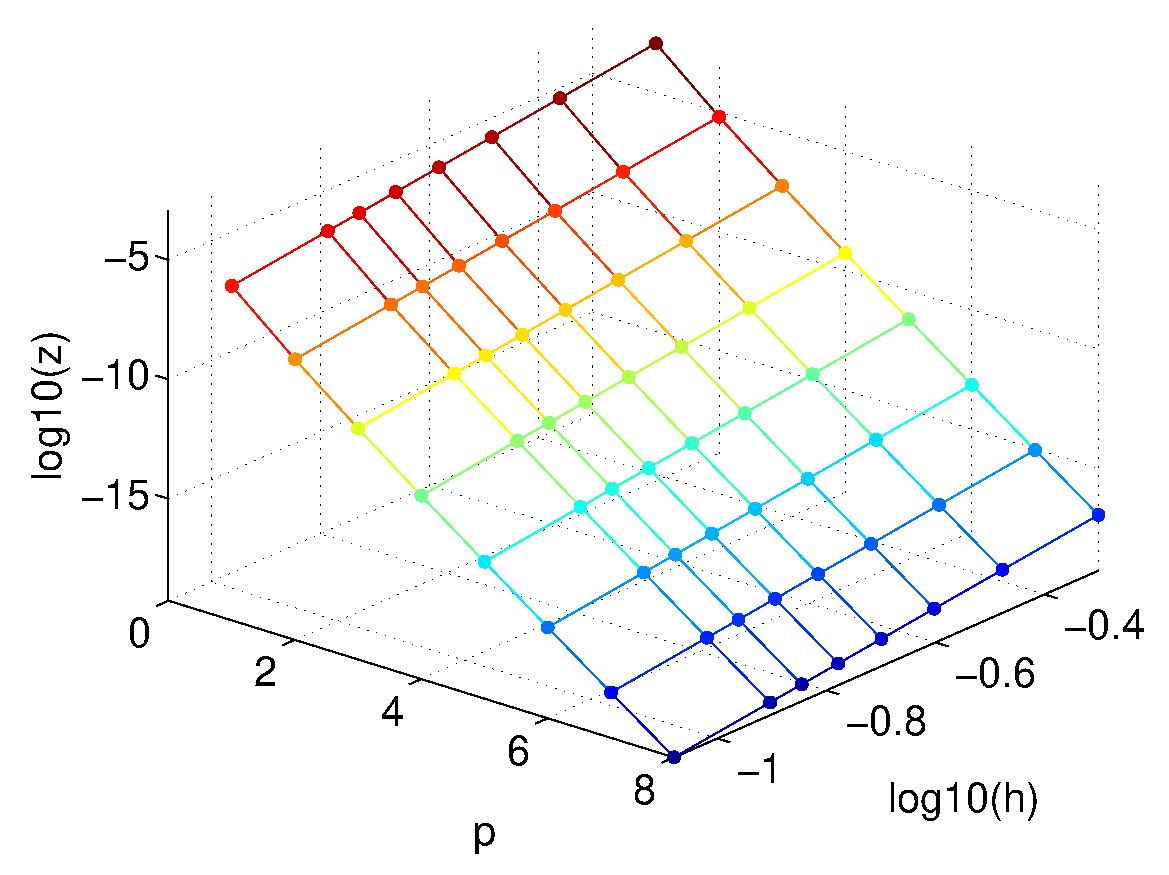
\includegraphics[width=0.45\textwidth]{Images/iga0_eigM3smin.eps}\\
\end{center}
\caption{At left, the numerically computed values of
$\lambda_{min}(M_0)$ for $d=3$ and
for different values of $h$ and $p$. At right,
the graphical representation of the r.h.s. of (\ref{eigminM_C0}). $c(3)
\simeq 1.7$}
\label{fig:massamin-iga0d3}
\end{figure}



\begin{figure}
\begin{center}
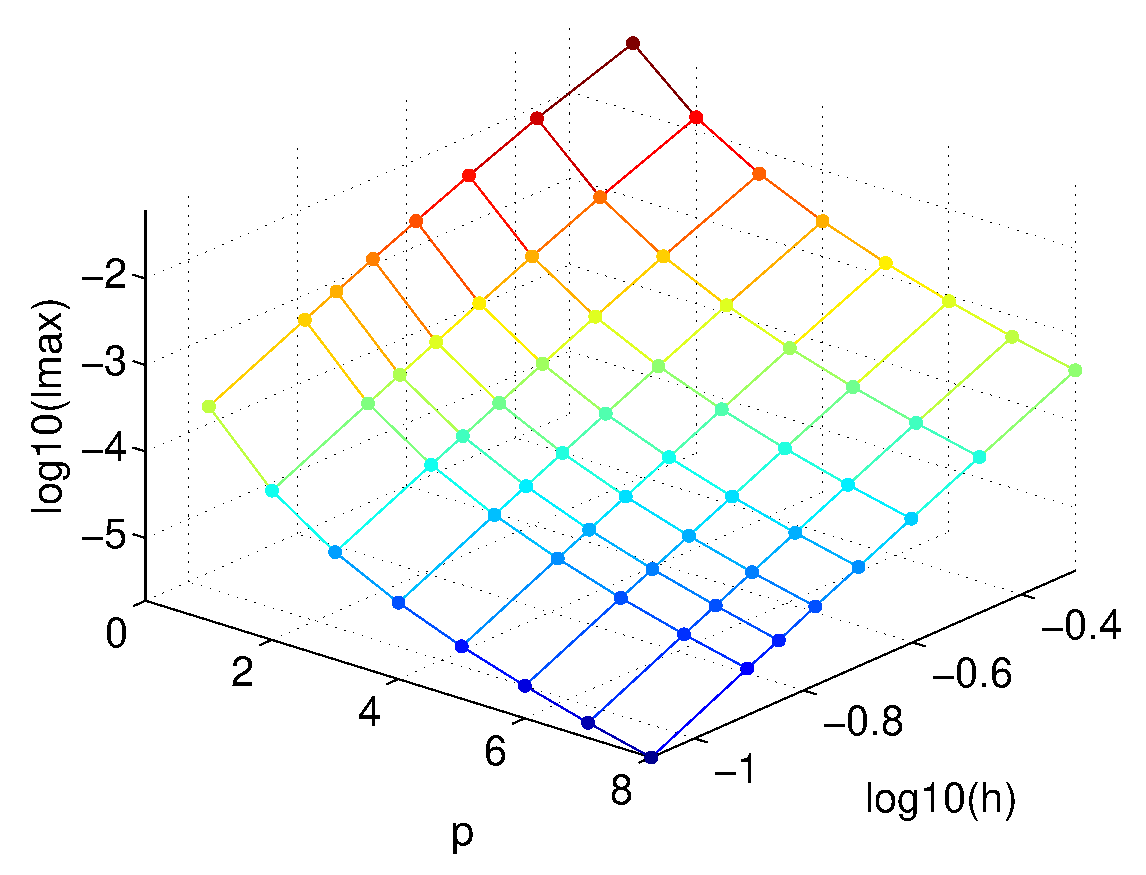
\includegraphics[width=0.45\textwidth]{Images/iga0_eigM3max.eps}\quad
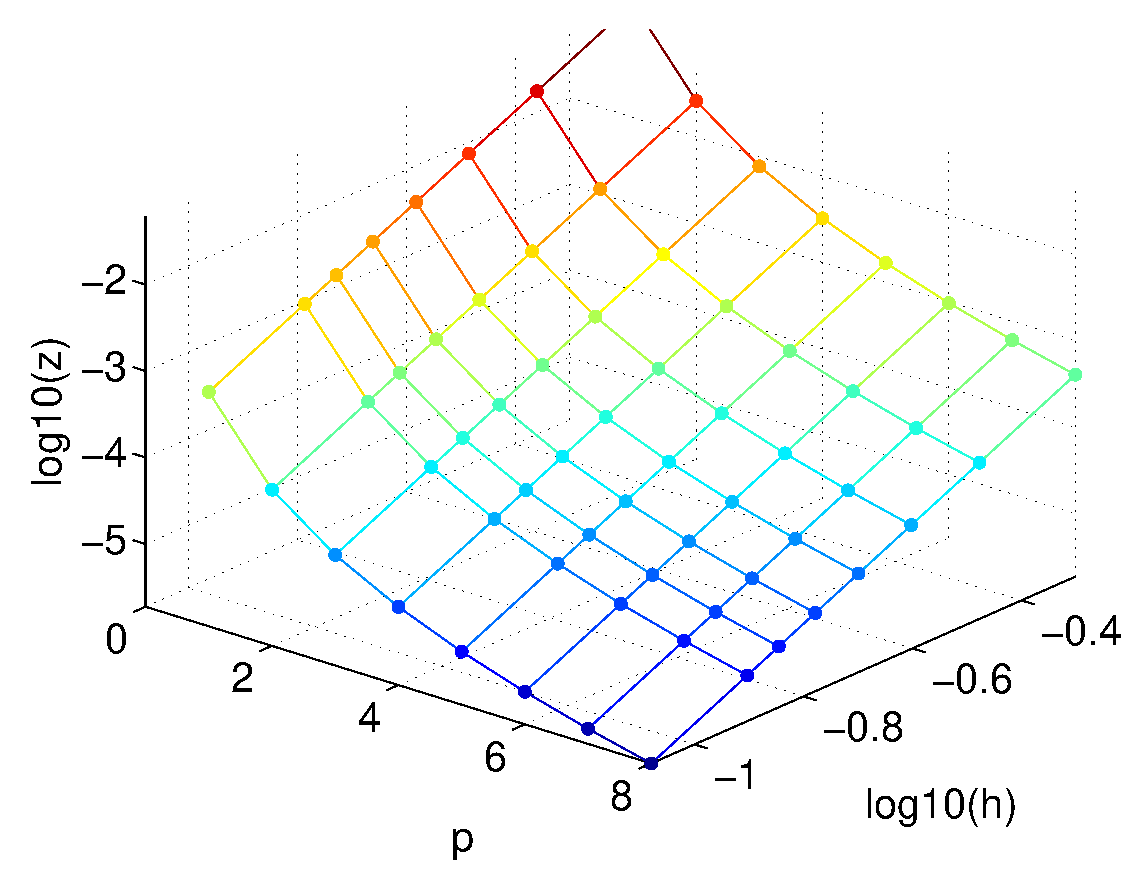
\includegraphics[width=0.45\textwidth]{Images/iga0_eigM3smax.eps}\\
\end{center}
\caption{At left, the numerically computed values of
$\lambda_{max}(M_0)$ for $d=3$ and
for different values of $h$ and $p$. At right,
the graphical representation of the r.h.s. of (\ref{eigmaxM_C0}). $c(3)
\simeq 1.7$}
\label{fig:massamax-iga0d3}
\end{figure}



\clearpage
\newpage
% ~~~~~~~~~~~~~~~~~~~~~~~~~~~~~~~~~
%  IGA-C0 stiff
% ~~~~~~~~~~~~~~~~~~~~~~~~~~~~~~~~~
\subsection{IGA-$C^0$ stiffness matrix}
Denoting by $K_0$ the stiffness matric corresponding to the 
IGA-$C^0$ approximation, its computed extreme eigenvalues
behave  depending  as follows (see also 
Fig. \ref{fig:stiff-iga0}):
\begin{eqnarray}
\label{eigminK_C0}
\lambda_{min}(K_0)&\sim &\left\{\begin{array}{ll}
c_1 h^dp^{-d} & \mbox{if } h\leq \left(\frac{c_2(d)}{c_1} p^de^{-1.3 d p}\right)^{1/2}\\
c_2(d)h^{d-2}e^{-1.3\,dp} &\mbox{otherwise}
\end{array}\right.\\
\label{eigmaxK_C0}
\lambda_{max}(K_0)&\sim &
\left\{\begin{array}{ll}
c_3 h^{d-2}p^{(1-d)/2} & \mbox{if } p\leq \overline{p}(d)\\
c_4h^{d-2}p^{2-d}  &\mbox{otherwise}
\end{array}\right.
\end{eqnarray}
for any $d=1,2,3$.  

The behaviour of the condition number ${\cal K}(K_0)$ versus both $h$ and
$p$ is shown in Fig. \ref{fig:stiffcond-iga0}


{\pg Dite che \`e il caso di togliere la distinzione $p><\overline{p}(d)$?

I risultati numerici sul 3d sono ancora incompleti, sto aspettando che finiscano
di girare, per\`o si hanno gi\`a buone conferme da quei pochi che ci sono.}




\begin{figure}[h]
\begin{center}
\scalebox{0.5}{\input{stiff_min_iga0.pdf_t}}\quad
\scalebox{0.5}{\input{stiff_max_iga0.pdf_t}}\quad
\end{center}
\caption{Behaviour of the extreme eigenvalues of the stiffness
 matrix of IGA-$C^0$ (logarithmic scale in $h$ is used)}
\label{fig:stiff-iga0}
\end{figure}

\begin{figure}[h]
\begin{center}
\scalebox{0.5}{\input{stiff_cond_iga0.pdf_t}}\quad
\end{center}
\caption{${\cal K}(K_{0})$ (logarithmic scale in $h$ is used)}
\label{fig:stiffcond-iga0}
\end{figure}

In Figures \ref{fig:stiffmin-iga0d1} -- \ref{fig:stiffmax-iga0d3} we show
the computed eigenvalues (at left) and the right hand sides of
(\ref{eigminK_C0}) --
(\ref{eigmaxK_C0}) w.r.t. $h$ and $p$. We deduce from numerical results
that $\overline{p}=2$ for $d=1$, $\overline{p}=3$ for $d=2$, and
$\overline{p}=0$ for $d=3$.

\begin{figure}[h]
\begin{center}
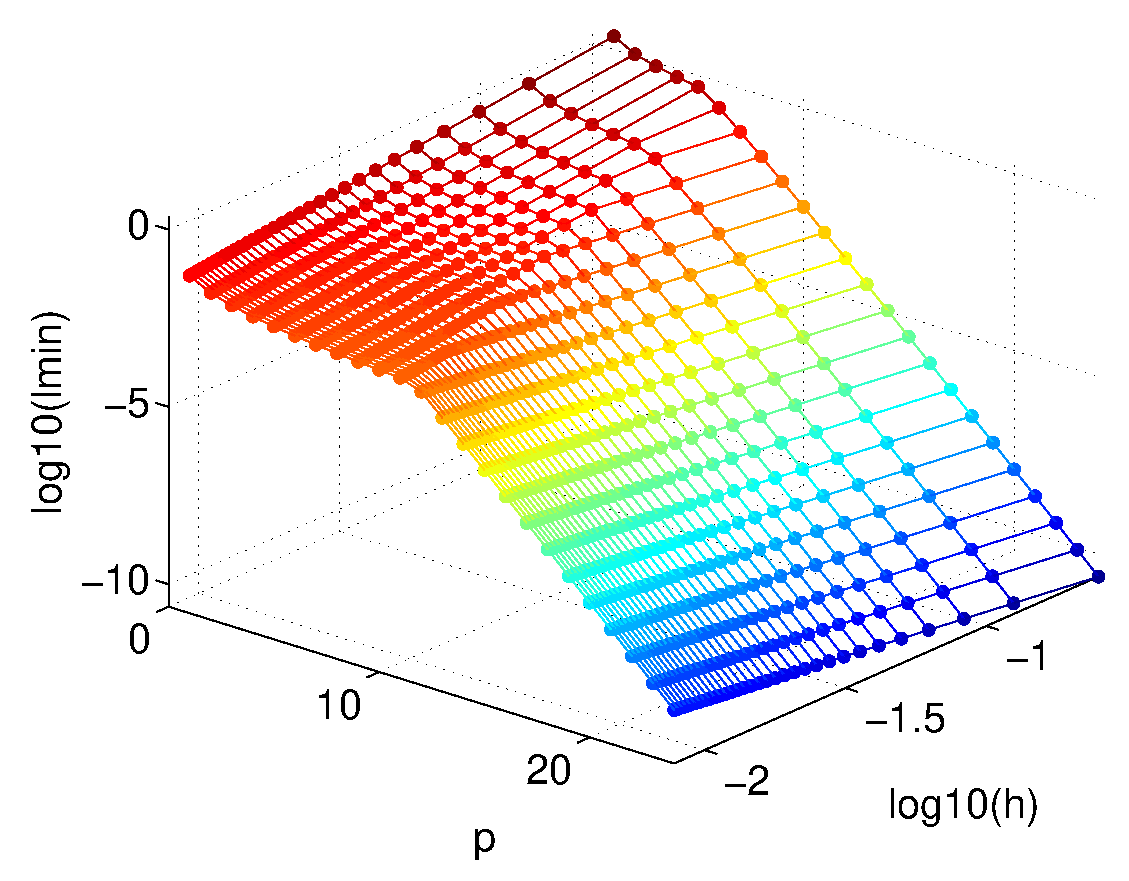
\includegraphics[width=0.45\textwidth]{Images/iga0_eigK1min.eps}\quad
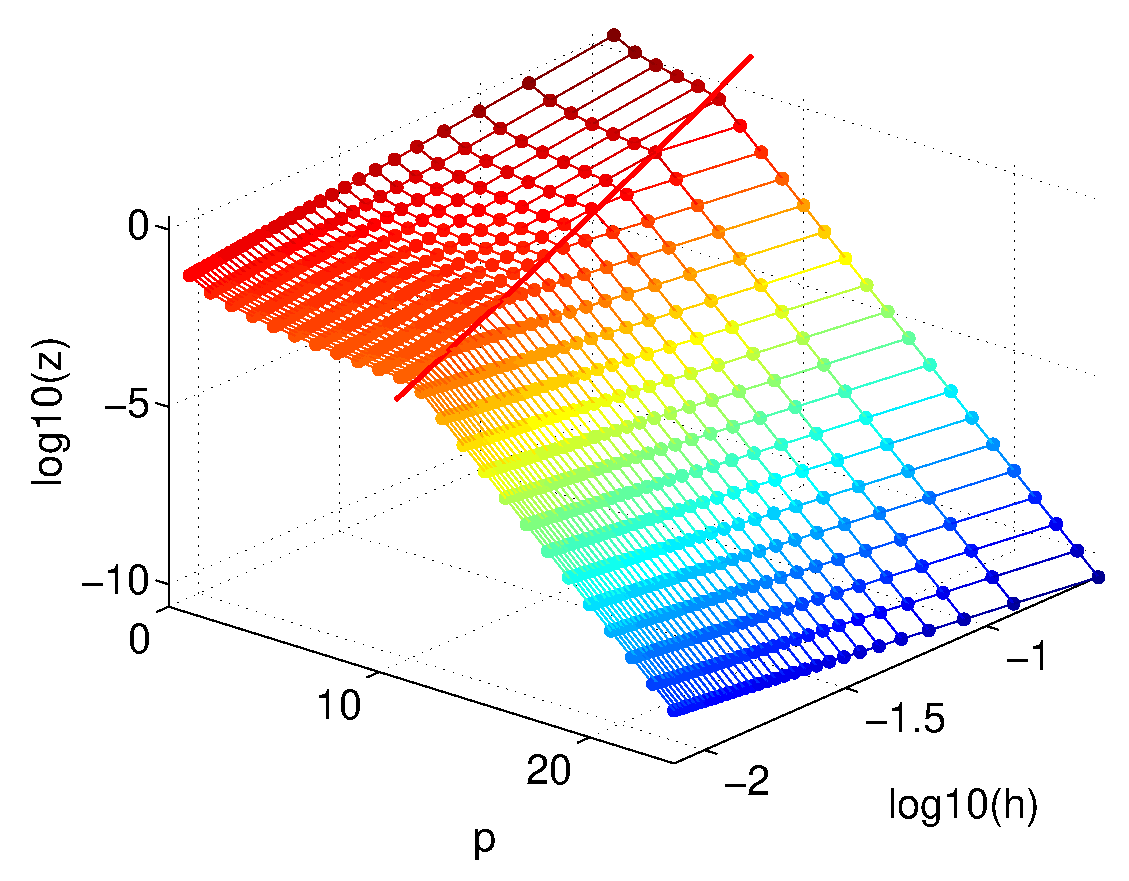
\includegraphics[width=0.45\textwidth]{Images/iga0_eigK1smin.eps}
\end{center}
\caption{At left, the numerically computed values of
$\lambda_{min}(K_0)$ for $d=1$ and
for different values of $h$ and $p$. At right,
the graphical representation of the r.h.s. of (\ref{eigminK_C0}). The red line
separates the two different regimes}
\label{fig:stiffmin-iga0d1}
\end{figure}

\begin{figure}
\begin{center}
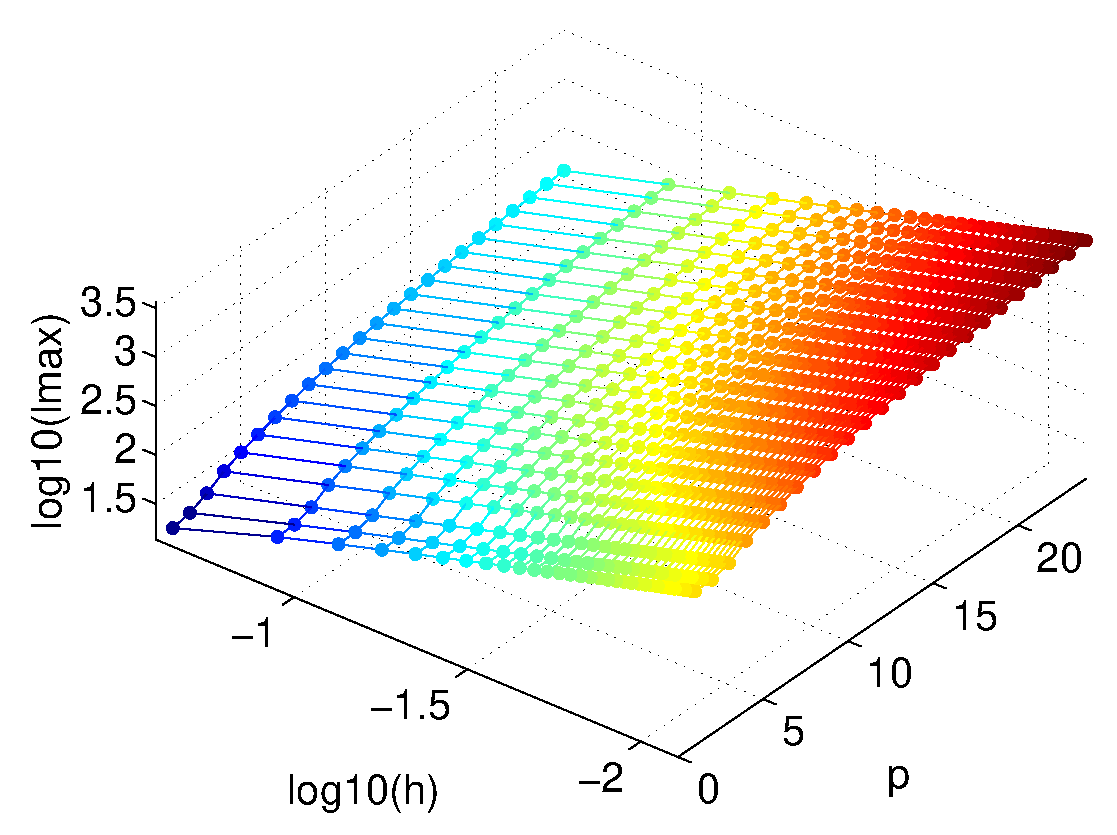
\includegraphics[width=0.45\textwidth]{Images/iga0_eigK1max.eps}\quad
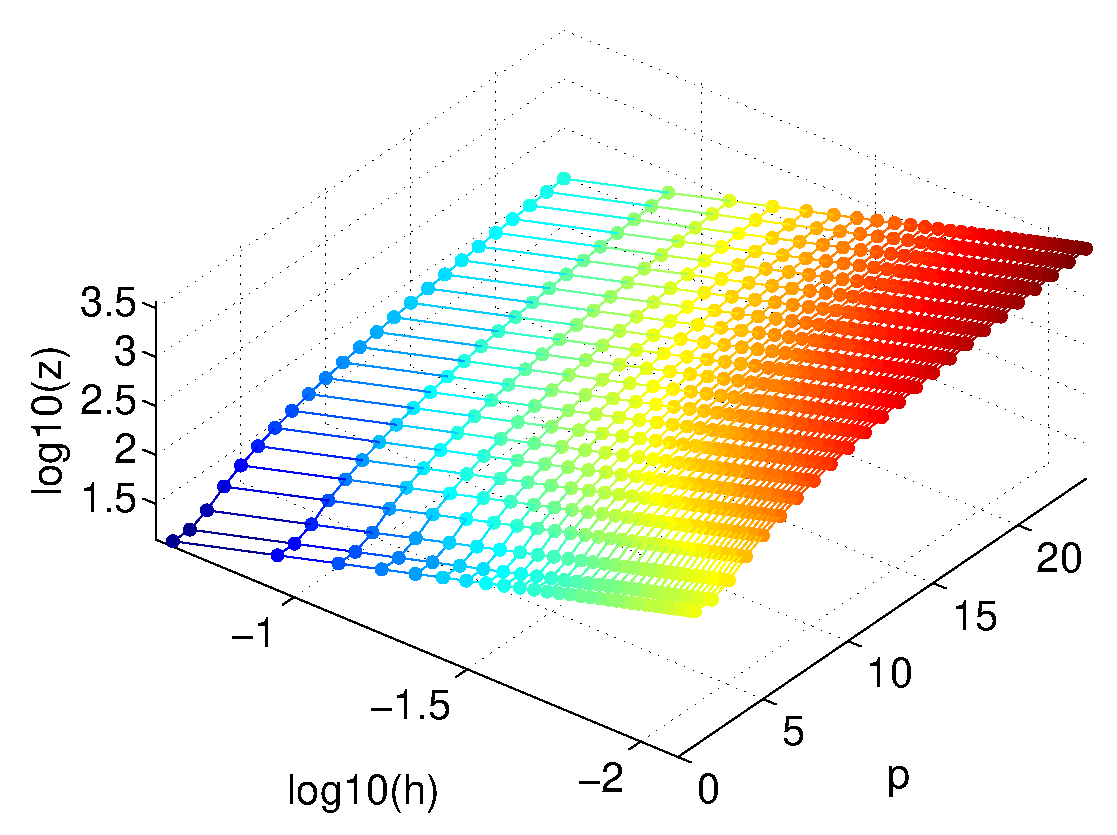
\includegraphics[width=0.45\textwidth]{Images/iga0_eigK1smax.eps}
\end{center}
\caption{At left, the numerically computed values of
$\lambda_{max}(K_0)$ for $d=1$ and
for different values of $h$ and $p$. At right,
the graphical representation of the r.h.s. of (\ref{eigmaxK_C0})}
\label{fig:stiffmax-iga0d1}
\end{figure}

\begin{figure}
\begin{center}
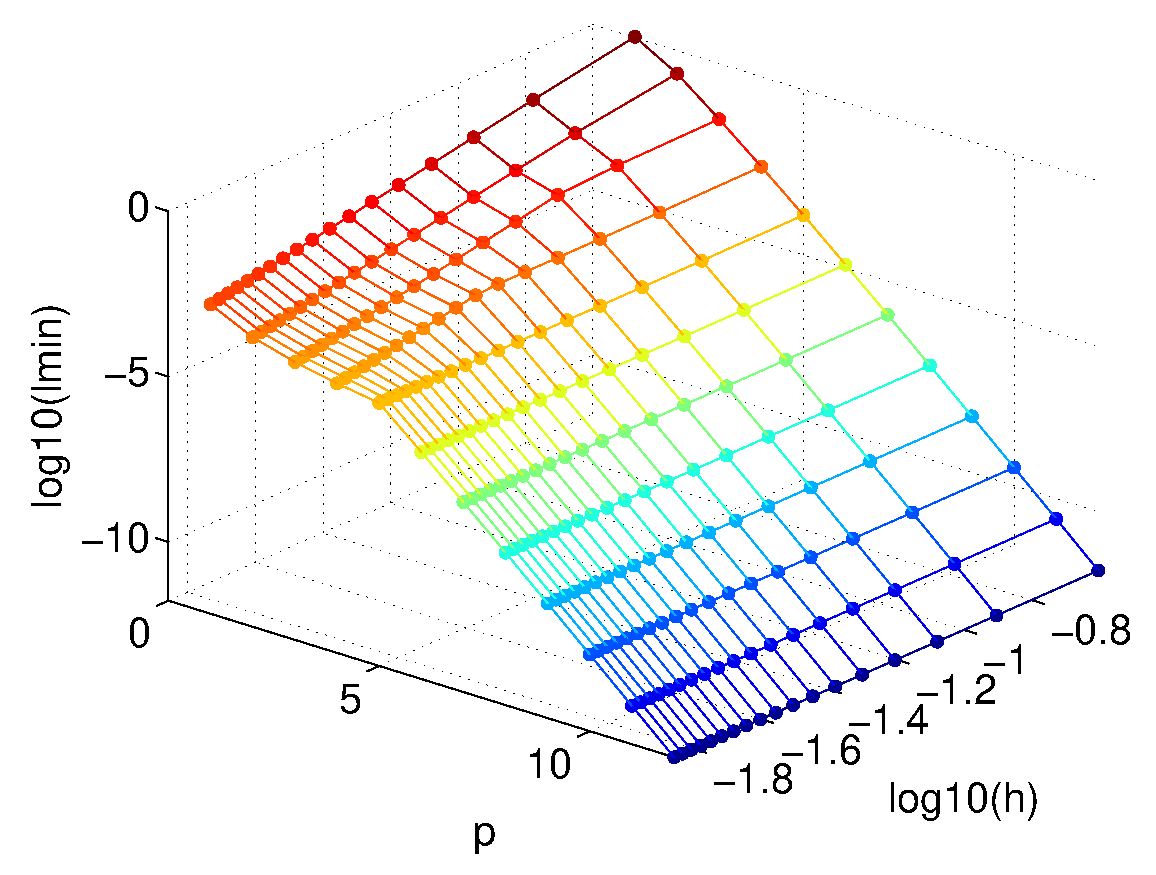
\includegraphics[width=0.45\textwidth]{Images/iga0_eigK2min.eps}\quad
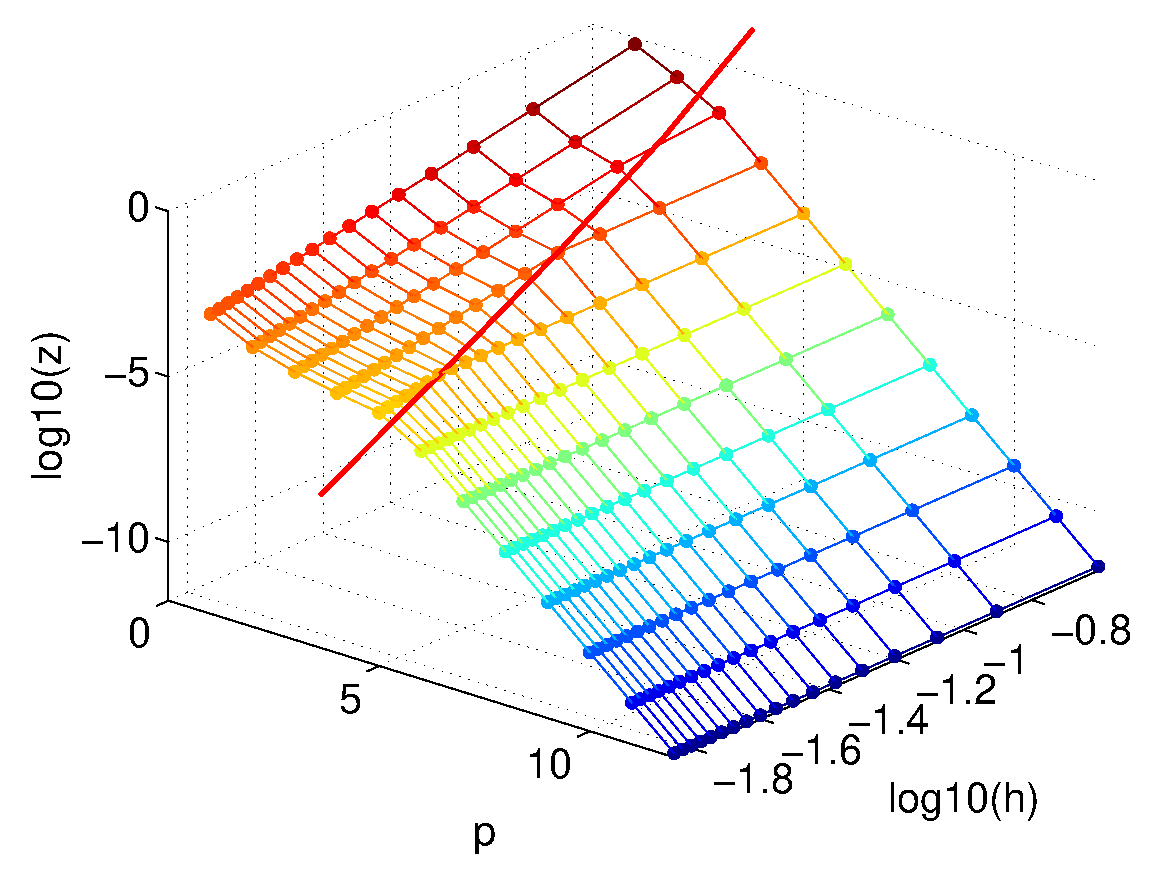
\includegraphics[width=0.45\textwidth]{Images/iga0_eigK2smin.eps}
\end{center}
\caption{At left, the numerically computed values of
$\lambda_{min}(K_0)$ for $d=2$ and
for different values of $h$ and $p$. At right,
the graphical representation of the r.h.s. of (\ref{eigminK_C0}). The red line
separates the two different regimes}
\label{fig:stiffmin-iga0d2}
\end{figure}

\begin{figure}
\begin{center}
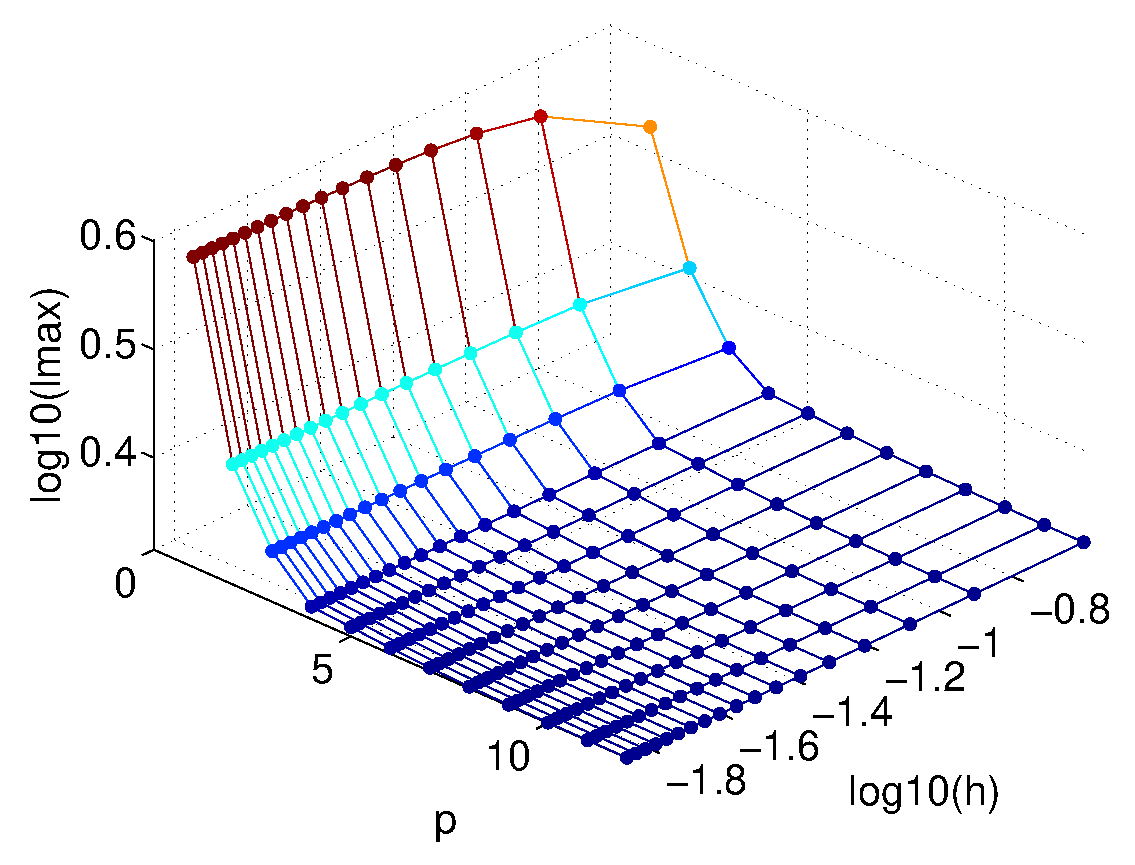
\includegraphics[width=0.45\textwidth]{Images/iga0_eigK2max.eps}\quad
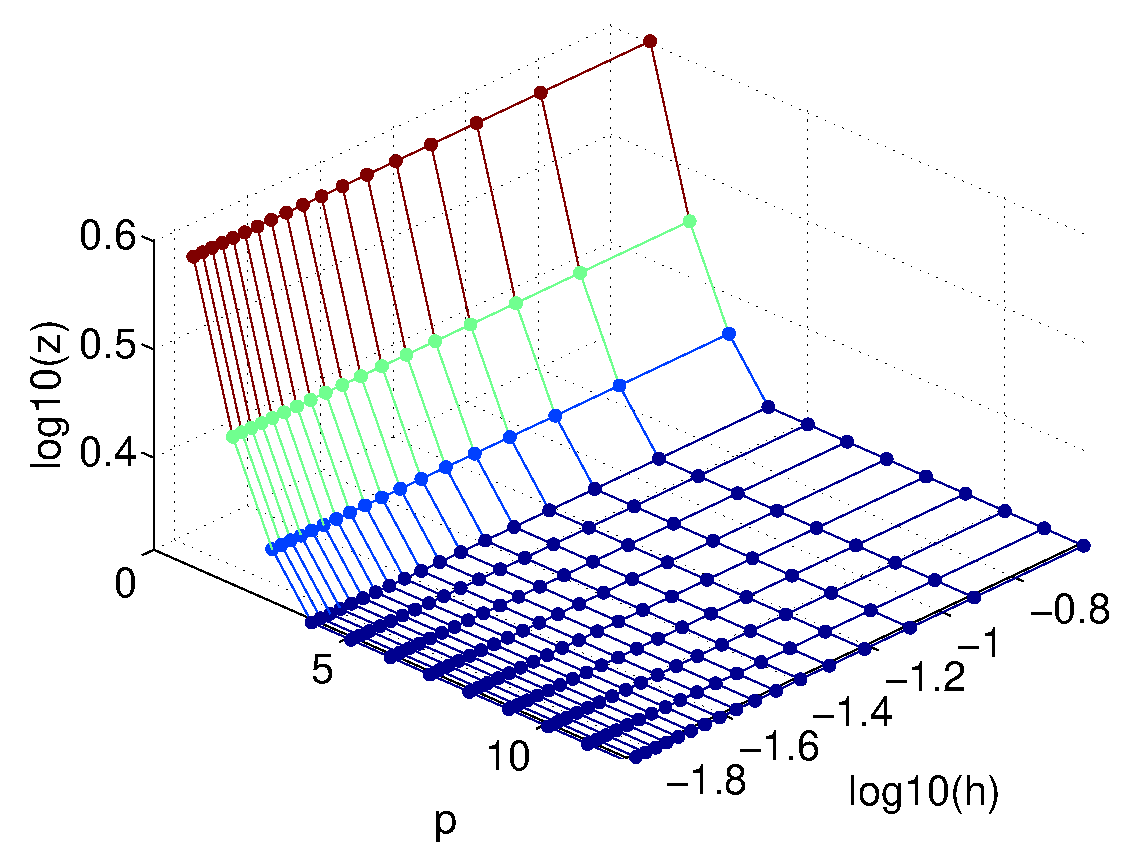
\includegraphics[width=0.45\textwidth]{Images/iga0_eigK2smax.eps}
\end{center}
\caption{At left, the numerically computed values of
$\lambda_{max}(K_0)$ for $d=2$ and
for different values of $h$ and $p$. At right,
the graphical representation of the r.h.s. of (\ref{eigmaxK_C0})}
\label{fig:stiffmax-iga0d2}
\end{figure}

\begin{figure}
\begin{center}
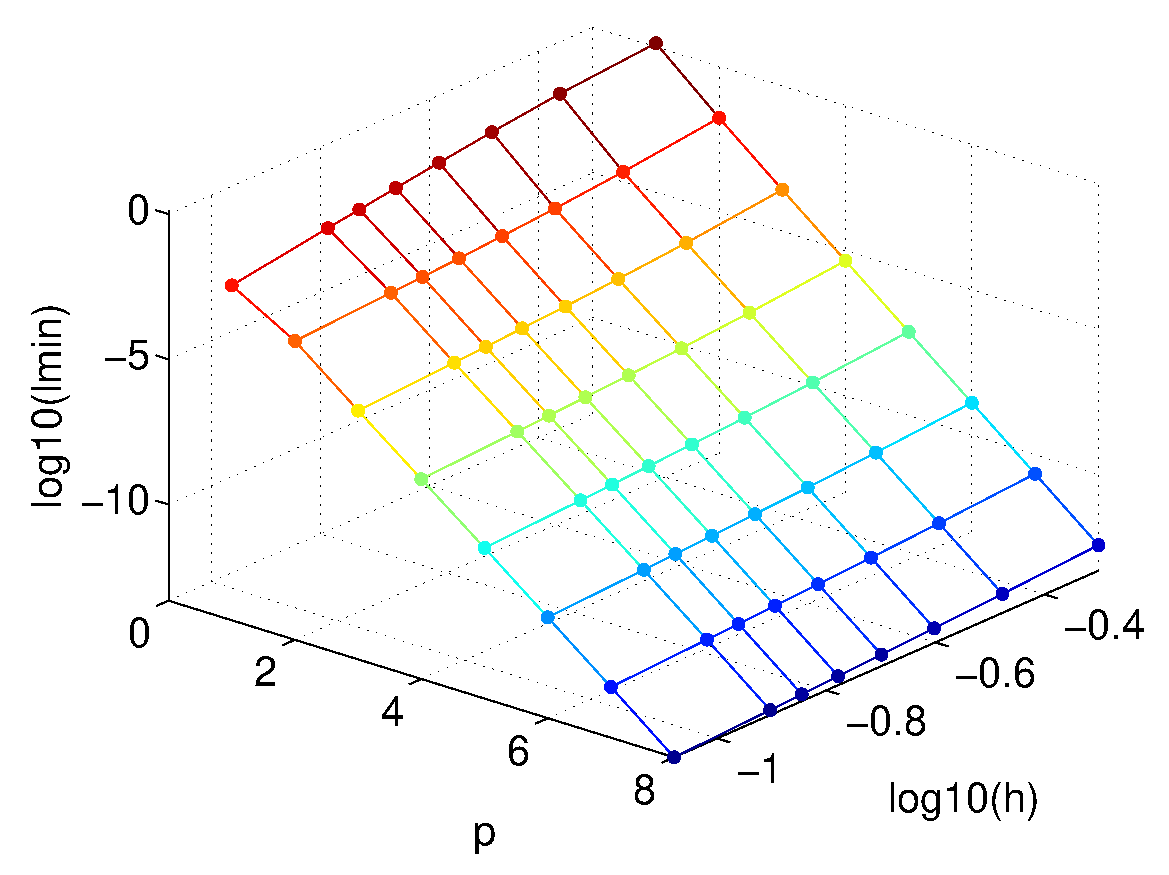
\includegraphics[width=0.45\textwidth]{Images/iga0_eigK3min.eps}\quad
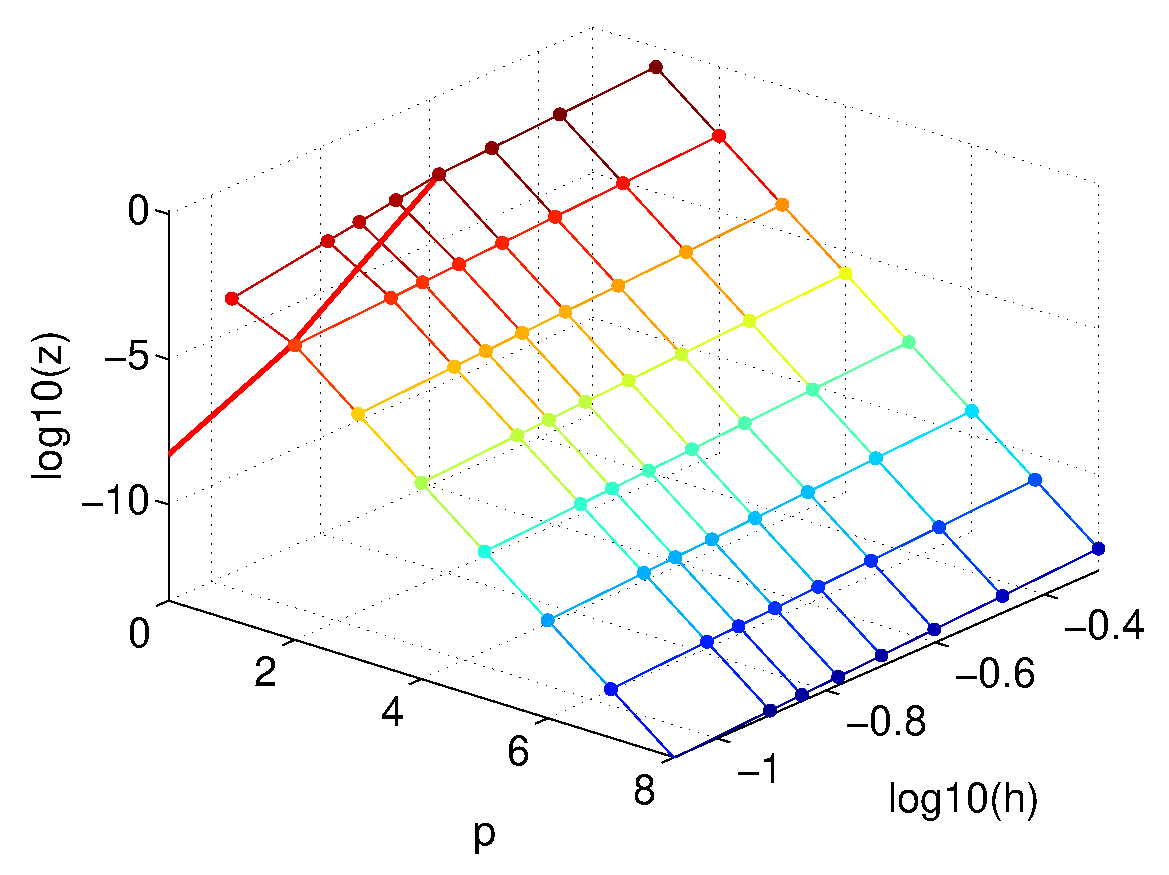
\includegraphics[width=0.45\textwidth]{Images/iga0_eigK3smin.eps}
\end{center}
\caption{At left, the numerically computed values of
$\lambda_{min}(K_0)$ for $d=3$ and
for different values of $h$ and $p$. At right,
the graphical representation of the r.h.s. of (\ref{eigminK_C0}). The red line
separates the two different regimes}
\label{fig:stiffmin-iga0d3}
\end{figure}

\begin{figure}
\begin{center}
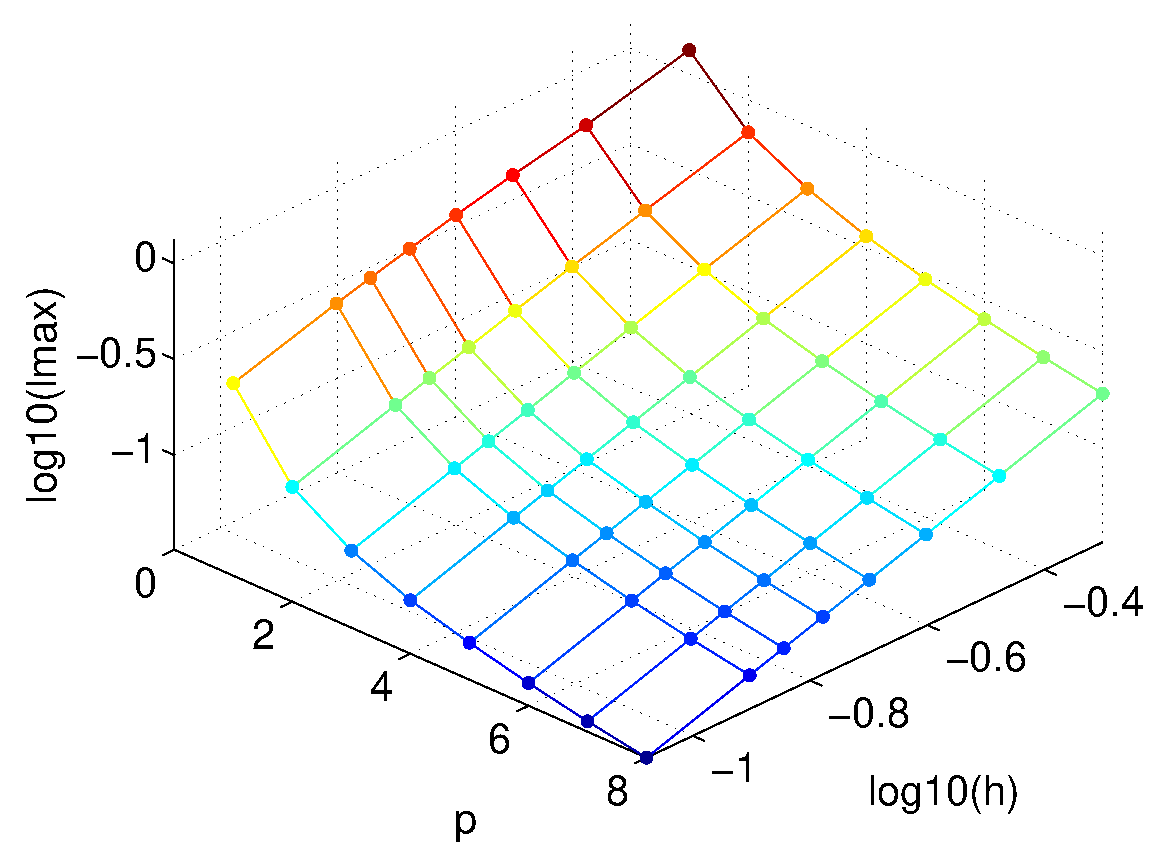
\includegraphics[width=0.45\textwidth]{Images/iga0_eigK3max.eps}\quad
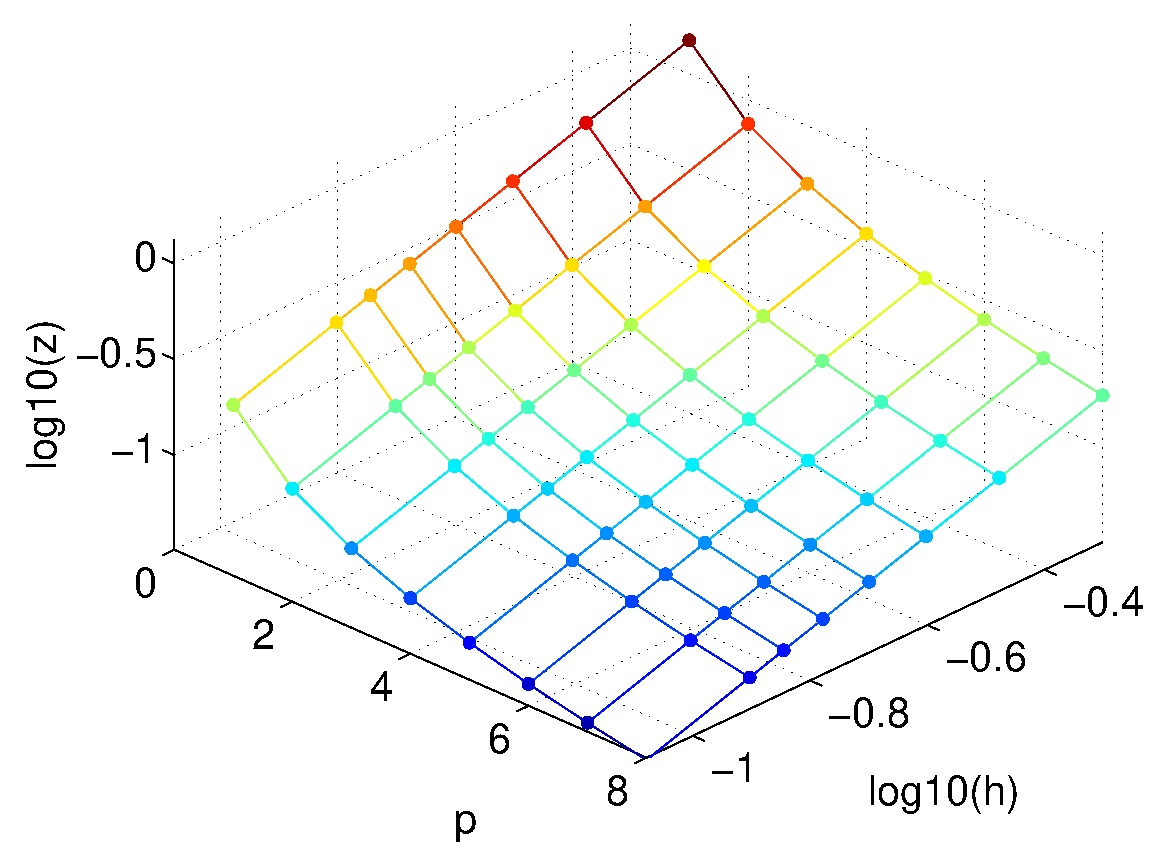
\includegraphics[width=0.45\textwidth]{Images/iga0_eigK3smax.eps}
\end{center}
\caption{At left, the numerically computed values of
$\lambda_{max}(K_0)$ for $d=3$ and
for different values of $h$ and $p$. At right,
the graphical representation of the r.h.s. of (\ref{eigmaxK_C0})}
\label{fig:stiffmax-iga0d3}
\end{figure}


\clearpage
\newpage
% ~~~~~~~~~~~~~~~~~~~~~~~~~~~~~~~~~
%  IGA-C0 M^{-1}A
% ~~~~~~~~~~~~~~~~~~~~~~~~~~~~~~~~~
\subsection{IGA-$C^0$ $(M^{-1}K)$ matrix}

The minimum eigenvalue of the                  
matrix $(M_0)^{-1}K_0$ of IGA-$C^0$
is  $\lambda_{min}((M_0)^{-1}K_0)\sim c$,
while the maximum on behaves like
\begin{equation} \label{eigmaxgen_C0}
\lambda_{max}((M_0)^{-1}K_0)\sim c(d) p^{3.5}h^{-2}
\end{equation}
independently of the dimension $d$. 
The constants behave as $c(d)\sim (4d+1)/2$.

In Figures \ref{fig:genmax-iga0d1} -- \ref{fig:genmax-iga0d3} we show
the numerically computed maximum eigenvalues (at left) and the right hand sides of
(\ref{eigmaxgen_C0}) w.r.t. $h$ and $p$. 

\begin{figure}[h]
\begin{center}
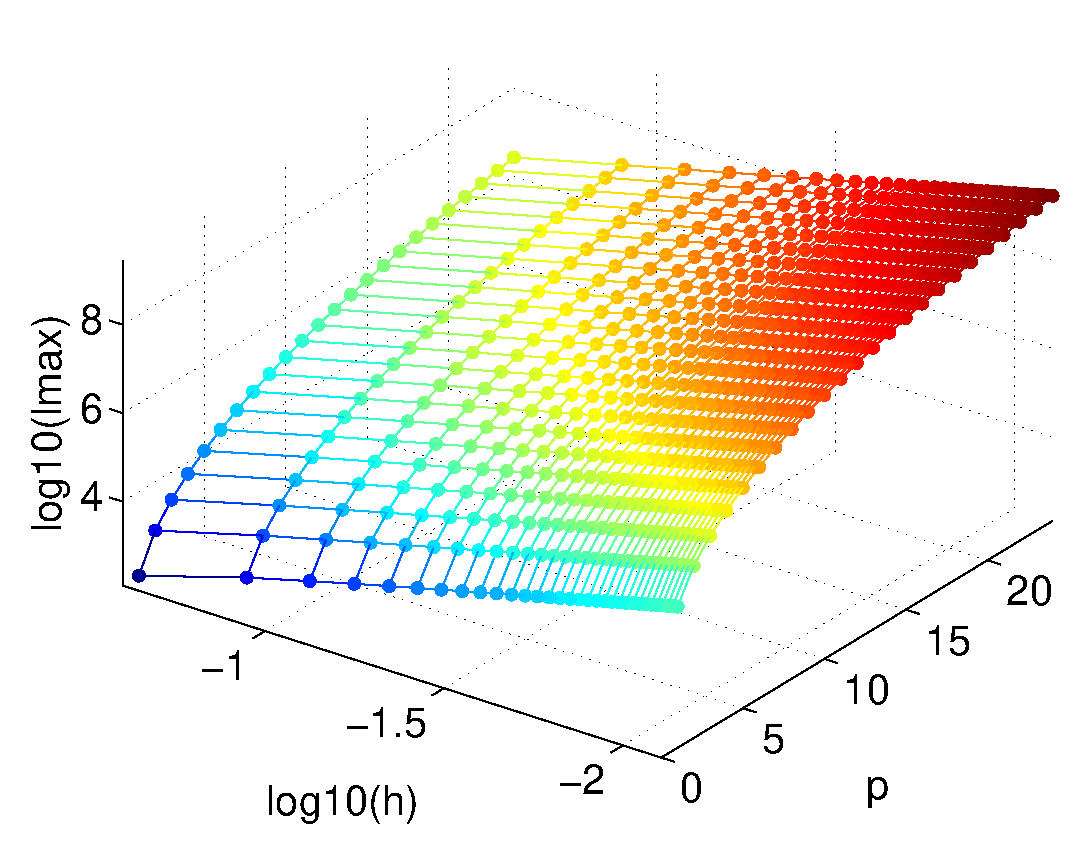
\includegraphics[width=0.45\textwidth]{Images/iga0_eiggen1max.eps}\quad
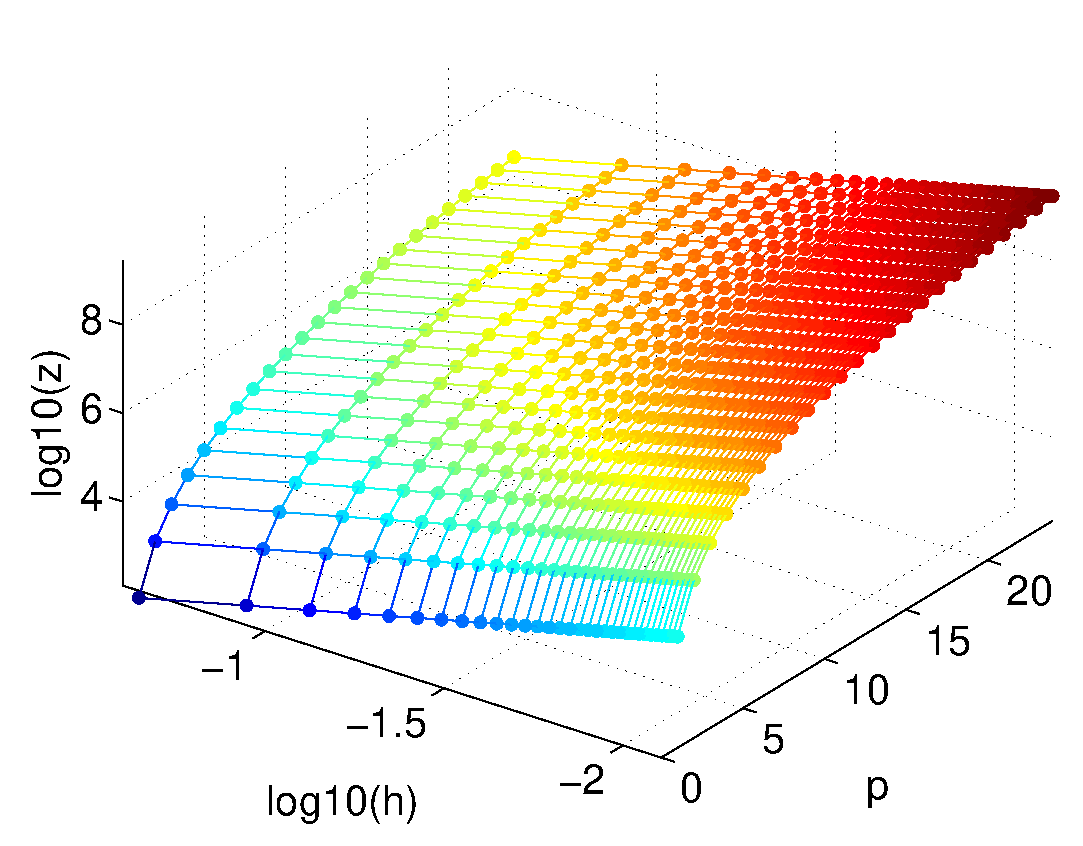
\includegraphics[width=0.45\textwidth]{Images/iga0_eiggen1smax.eps}
\end{center}
\caption{At left, the numerically computed values of
$\lambda_{max}((M_0)^{-1}K_0)$ for $d=1$ and
for different values of $h$ and $p$. At right,
the graphical representation of the r.h.s. of (\ref{eigmaxgen_C0})}
\label{fig:genmax-iga0d1}
\end{figure}

\begin{figure}
\begin{center}
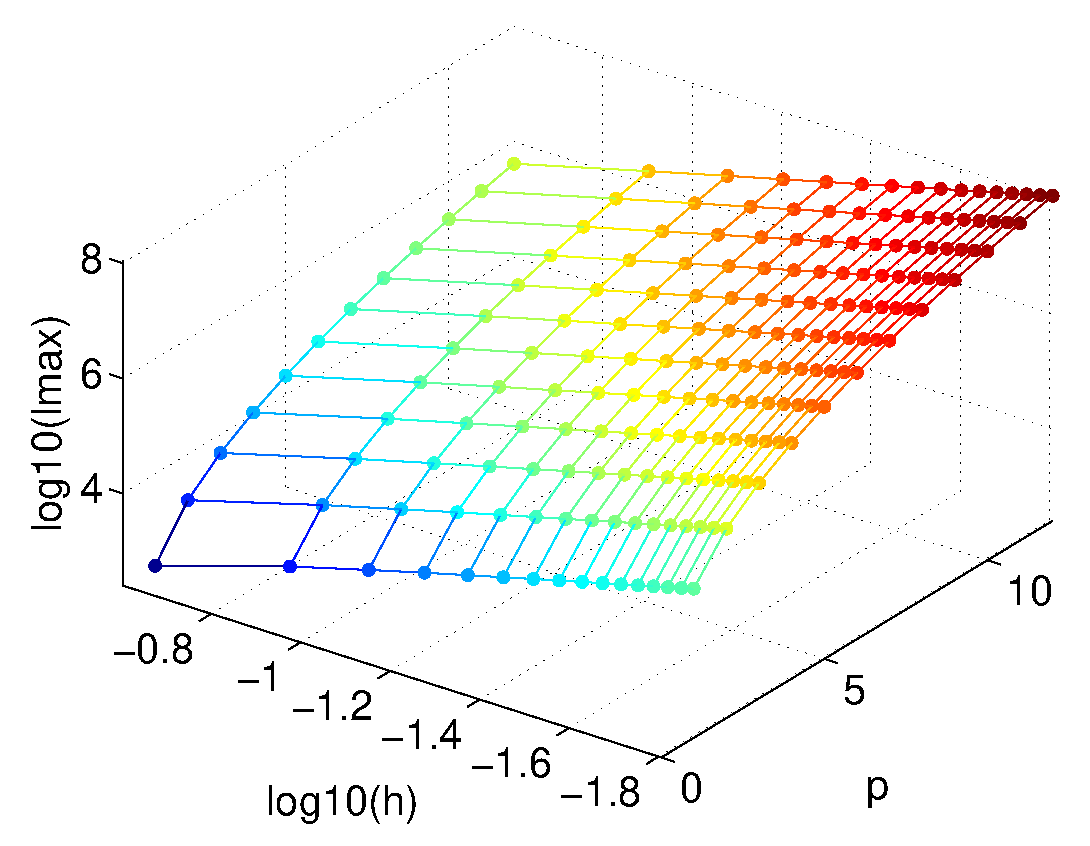
\includegraphics[width=0.45\textwidth]{Images/iga0_eiggen2max.eps}\quad
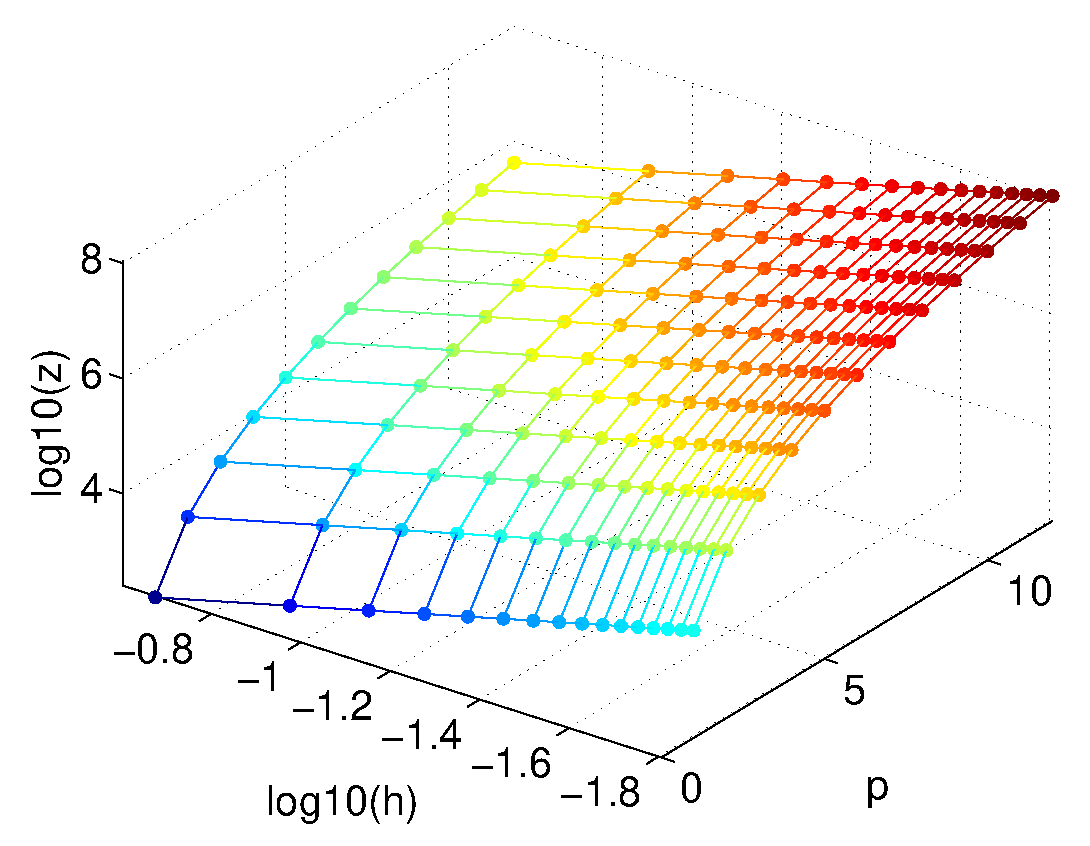
\includegraphics[width=0.45\textwidth]{Images/iga0_eiggen2smax.eps}
\end{center}
\caption{At left, the numerically computed values of
$\lambda_{max}((M_0)^{-1}K_0)$ for $d=2$ and
for different values of $h$ and $p$. At right,
the graphical representation of the r.h.s. of (\ref{eigmaxgen_C0})}
\label{fig:genmax-iga0d2}
\end{figure}

\begin{figure}
\begin{center}
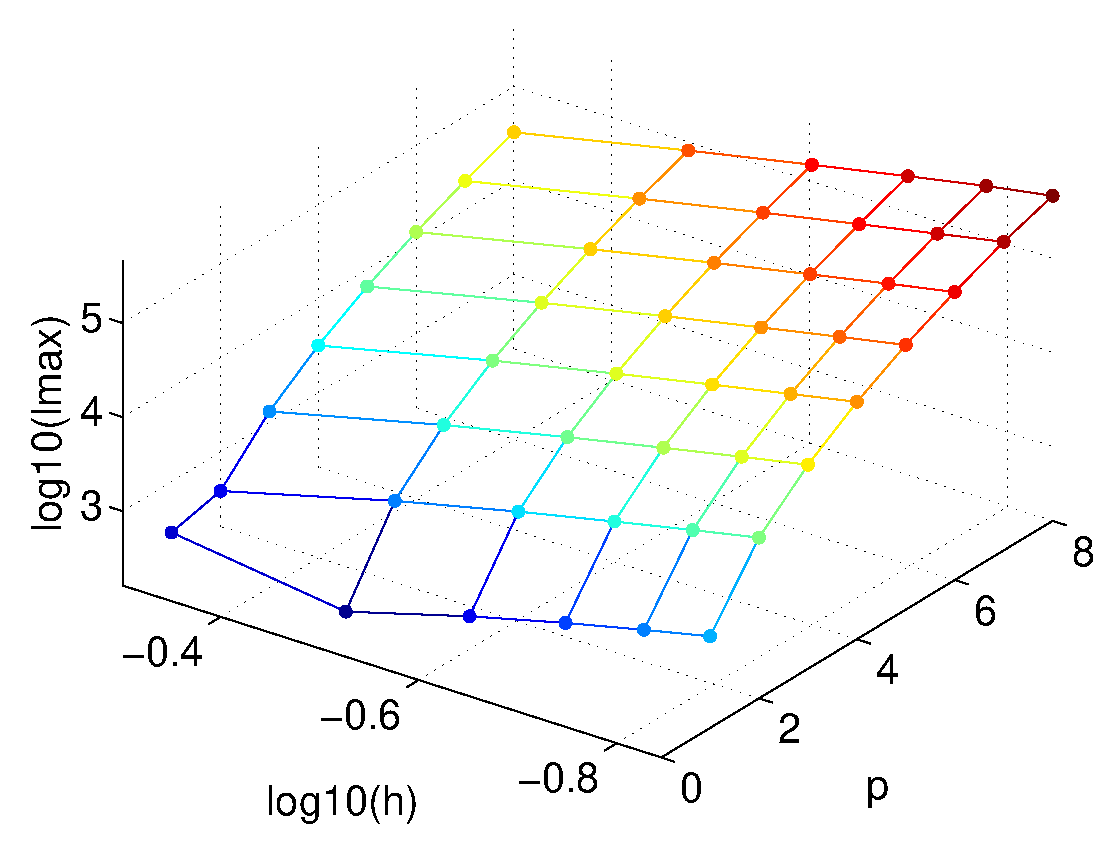
\includegraphics[width=0.45\textwidth]{Images/iga0_eiggen3max.eps}\quad
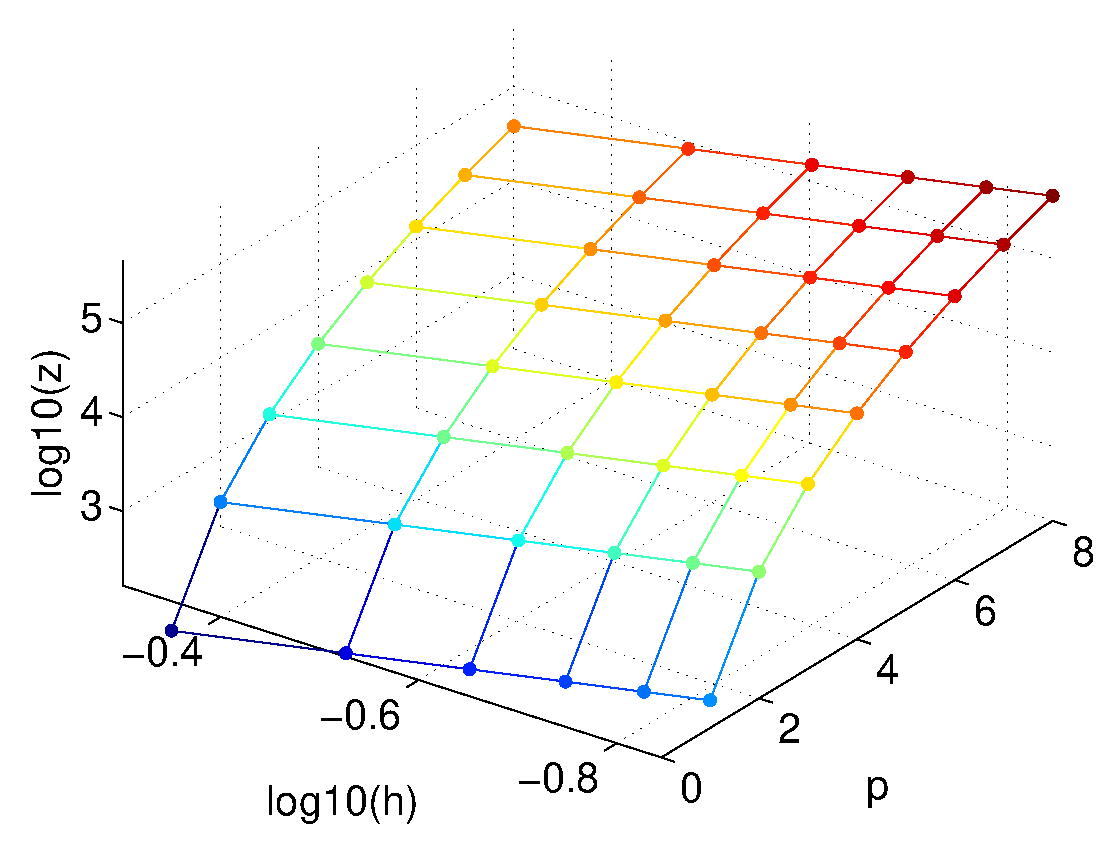
\includegraphics[width=0.45\textwidth]{Images/iga0_eiggen3smax.eps}
\end{center}
\caption{At left, the numerically computed values of
$\lambda_{max}((M_0)^{-1}K_0)$ for $d=3$ and
for different values of $h$ and $p$. At right,
the graphical representation of the r.h.s. of (\ref{eigmaxgen_C0})}
\label{fig:genmax-iga0d3}
\end{figure}


\clearpage
\newpage

% ~~~~~~~~~~~~~~~~~~~~~~~~~~~~~~~~~~
% IGA-C(p-1)  mass
% ~~~~~~~~~~~~~~~~~~~~~~~~~~~~~~~~~~
\subsection{IGA-$C^{p-1}$ mass matrix}


The extreme eigenvalues of the
mass matrix $M_{p-1}$ of IGA-$C^{p-1}$,
behave depending on $h$ and $p$, as follows (see also
Fig. \ref{fig:mass-igap}):
\begin{eqnarray}
\label{eigminM_Cp}
\lambda_{min}(M_{p-1})&\sim &\left\{\begin{array}{ll}
h^d e^{-pd}& \mbox{if } h\leq 1/p\\
\left(\frac{e}{4}\right)^{-d/h}p^{-d}4^{-pd}&\mbox{otherwise}
\end{array}\right.\\
\label{eigmaxM_Cp}
\lambda_{max}(M_{p-1})&\sim &
\left\{\begin{array}{ll}
h^d & \mbox{if } h\leq 1/p\\
p^{-d}  &\mbox{otherwise}
\end{array}\right.
\end{eqnarray}
for any $d=1,2,3$. 

The spectral condition number reads
\begin{eqnarray}
\label{cond_M_Cp}
{\cal K}(M_{p-1})&\sim &\left\{\begin{array}{ll}
 e^{pd}& \mbox{if } h\leq 1/p\\
\left(\frac{e}{4}\right)^{d/h}4^{pd}&\mbox{otherwise.}
\end{array}\right.
\end{eqnarray}

\begin{figure}[h]
\begin{center}
\scalebox{0.5}{\input{massa_igap.pdf_t}}
\end{center}
\caption{Behaviour of the extreme eigenvalues of the stiffness
 matrix of IGA-$C^{p-1}$ (logarithmic scale in $h$ is used)}
\label{fig:mass-igap}
\end{figure}


In Figures \ref{fig:massmin-igapd1} -- \ref{fig:massmax-igapd3} we show
the numerically computed eigenvalues (at left) and the right hand sides of
(\ref{eigminM_Cp}) --
(\ref{eigmaxM_Cp}) w.r.t. $h$ and $p$.

\begin{figure}[h]
\begin{center}
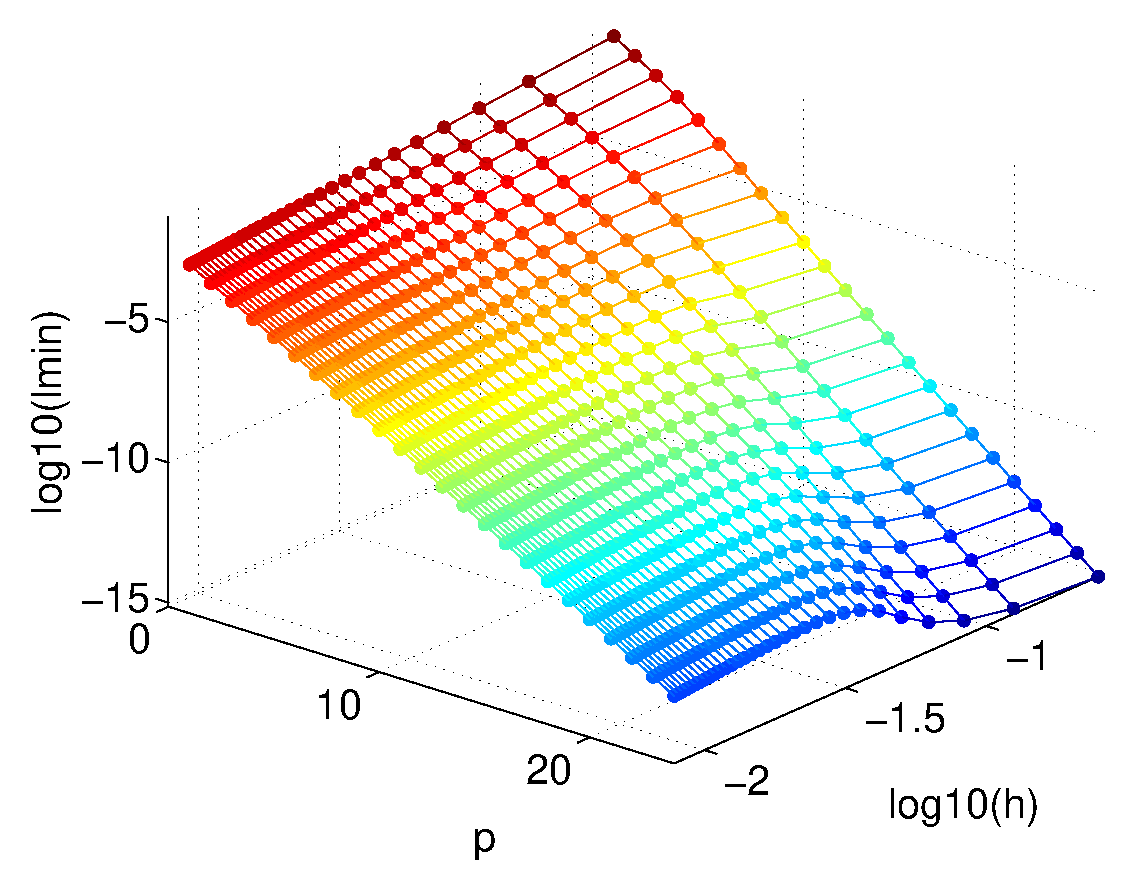
\includegraphics[width=0.45\textwidth]{Images/igap_eigM1min.eps}\quad
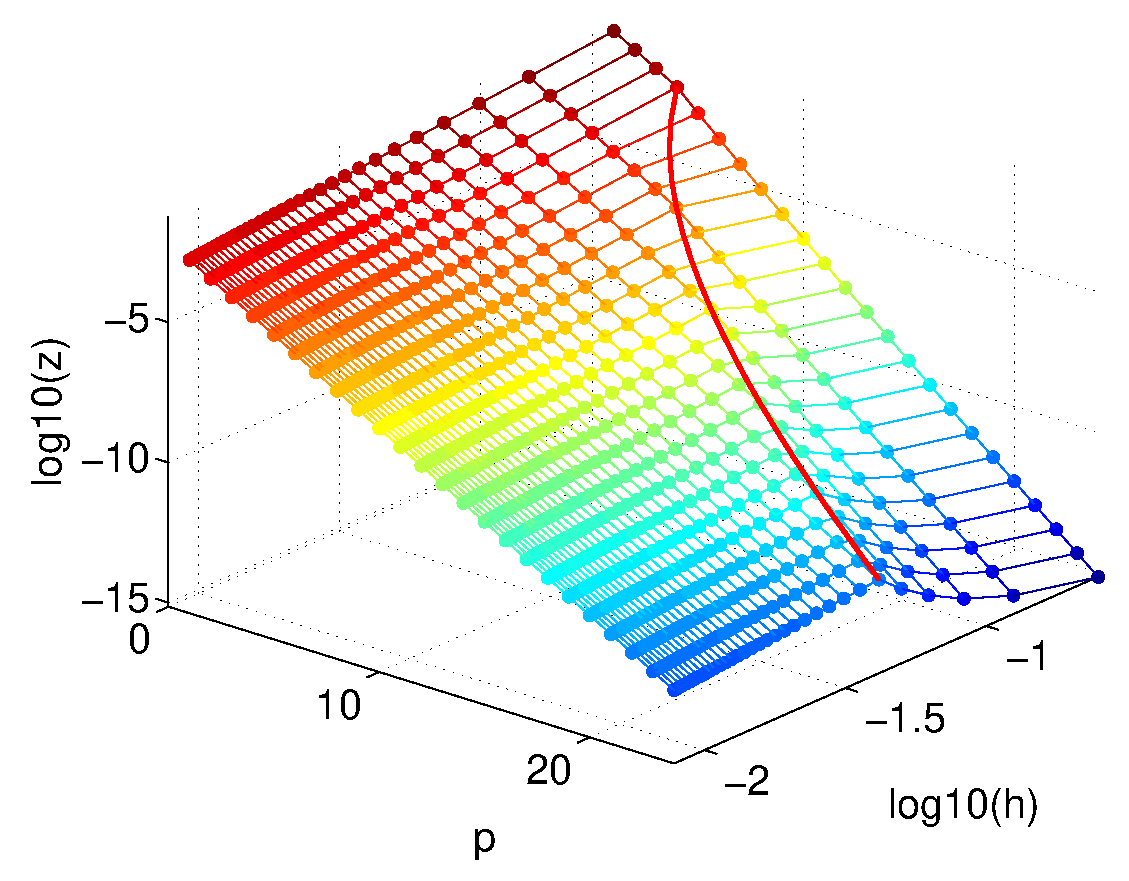
\includegraphics[width=0.45\textwidth]{Images/igap_eigM1smin.eps}\\
\end{center}
\caption{At left, the numerically computed values of
$\lambda_{min}(M_{p-1})$ for $d=1$ and
for different values of $h$ and $p$. At right,
the graphical representation of the r.h.s. of (\ref{eigminM_Cp}). The red line
separates the two different regimes}
\label{fig:massmin-igapd1}
\end{figure}

\begin{figure}
\begin{center}
\includegraphics[width=0.45\textwidth]{Images/igap_eigM1max.eps}\quad
\includegraphics[width=0.45\textwidth]{Images/igap_eigM1smax.eps}\\
\end{center}
\caption{At left, the numerically computed values of
$\lambda_{max}(M_{p-1})$ for $d=1$ and
for different values of $h$ and $p$. At right,
the graphical representation of the r.h.s. of (\ref{eigmaxM_Cp})}
\label{fig:massmax-igapd1}
\end{figure}

\begin{figure}
\begin{center}
\includegraphics[width=0.45\textwidth]{Images/igap_eigM2min.eps}\quad
\includegraphics[width=0.45\textwidth]{Images/igap_eigM2smin.eps}\\
\end{center}
\caption{At left, the numerically computed values of
$\lambda_{min}(M_{p-1})$ for $d=2$ and
for different values of $h$ and $p$. At right,
the graphical representation of the r.h.s. of (\ref{eigminM_Cp}). The red line
separates the two different regimes}
\label{fig:massmin-igapd2}
\end{figure}

\begin{figure}
\begin{center}
\includegraphics[width=0.45\textwidth]{Images/igap_eigM2max.eps}\quad
\includegraphics[width=0.45\textwidth]{Images/igap_eigM2smax.eps}\\
\end{center}
\caption{At left, the numerically computed values of
$\lambda_{max}(M_{p-1})$ for $d=2$ and
for different values of $h$ and $p$. At right,
the graphical representation of the r.h.s. of (\ref{eigmaxM_Cp})}
\label{fig:massmax-igapd2}
\end{figure}

\begin{figure}
\begin{center}
\includegraphics[width=0.45\textwidth]{Images/igap_eigM3min.eps}\quad
\includegraphics[width=0.45\textwidth]{Images/igap_eigM3smin.eps}\\
\end{center}
\caption{At left, the numerically computed values of
$\lambda_{min}(M_{p-1})$ for $d=3$ and
for different values of $h$ and $p$. At right,
the graphical representation of the r.h.s. of (\ref{eigminM_Cp}). The red line
separates the two different regimes}
\label{fig:massmin-igapd3}
\end{figure}

\begin{figure}
\begin{center}
\includegraphics[width=0.45\textwidth]{Images/igap_eigM3max.eps}\quad
\includegraphics[width=0.45\textwidth]{Images/igap_eigM3smax.eps}\\
\end{center}
\caption{At left, the numerically computed values of
$\lambda_{max}(M_{p-1})$ for $d=3$ and
for different values of $h$ and $p$. At right,
the graphical representation of the r.h.s. of (\ref{eigmaxM_Cp})}
\label{fig:massmax-igapd3}
\end{figure}

\clearpage
\newpage
% ~~~~~~~~~~~~~~~~~~~~~~~~~~~~~~~~~~
% IGA-C(p-1)  stiff
% ~~~~~~~~~~~~~~~~~~~~~~~~~~~~~~~~~~
\subsection{IGA-$C^{p-1}$ stiffness matrix}

The extreme eigenvalues of the
stiffness matrix $K_{p-1}$ of IGA-$C^{p-1}$,
behave depending on $h$ and $p$, as follows (see also
Fig. \ref{fig:mass-igap}):
\begin{eqnarray}
\label{eigminK_Cp}
\lambda_{min}(K_{p-1})&\sim &\left\{\begin{array}{ll}
ch^d& \mbox{if } h\leq e^{-pd/2}\\
ch^{d-2} e^{-pd}& \mbox{if }  e^{-pd/2}\leq h\leq 1/p\\
c \left(\frac{e}{4}\right)^{-d/h}p^{2-d}4^{-pd}&\mbox{if }h>1/p
\end{array}\right.\\
\label{eigmaxK_Cp}
\lambda_{max}(K_{p-1})&\sim &
\left\{\begin{array}{ll}
ch^{d-2} & \mbox{if } p=1\\
c ph^{d-2} & \mbox{if } p\geq 2 \mbox{ and } h\leq 1/p\\
c p^{2-d}h^{-1}  & \mbox{if } p\geq 2 \mbox{ and } h> 1/p
\end{array}\right.
\end{eqnarray}
for any $d=1,2,3$. 

The behaviour of the condition number ${\cal K}(K_{p-1})$ versus both $h$ and 
$p$ is shown in Fig. \ref{fig:stiffcond-igap}

\begin{figure}[h]
\begin{center}
\scalebox{0.5}{\input{stiff_min_igap.pdf_t}}\quad
\scalebox{0.5}{\input{stiff_max_igap.pdf_t}}\quad
\end{center}
\caption{Stiffness matrix for IGA-$C^{p-1}$ (logarithmic scale in $h$ is used)}
\label{fig:stiff-igap}
\end{figure}

\begin{figure}[h]
\begin{center}
\scalebox{0.5}{\input{stiff_cond_igap.pdf_t}}\quad
\end{center}
\caption{${\cal K}(K_{p-1})$ (logarithmic scale in $h$ is used)}
\label{fig:stiffcond-igap}
\end{figure}



\begin{figure}[h]
\begin{center}
\includegraphics[width=0.45\textwidth]{Images/igap_eigK1min.eps}\quad
\includegraphics[width=0.45\textwidth]{Images/igap_eigK1smin.eps}\\
\end{center}
\caption{At left, the numerically computed values of
$\lambda_{min}(K_{p-1})$ for $d=1$ and
for different values of $h$ and $p$. At right,
the graphical representation of the right hand side of (\ref{eigminK_Cp}). The red line
separates the two different regimes}
\label{fig:stiffmin-igapd1}
\end{figure}

\begin{figure}
\begin{center}
\includegraphics[width=0.45\textwidth]{Images/igap_eigK1max.eps}\quad
\includegraphics[width=0.45\textwidth]{Images/igap_eigK1smax.eps}\\
\end{center}
\caption{At left, the numerically computed values of
$\lambda_{max}(K_{p-1})$ for $d=1$ and
for different values of $h$ and $p$. At right,
the graphical representation of the r.h.s. of (\ref{eigmaxK_Cp})}
\label{fig:stiffmax-igapd1}
\end{figure}
\begin{figure}
\begin{center}
\includegraphics[width=0.45\textwidth]{Images/igap_eigK2min.eps}\quad
\includegraphics[width=0.45\textwidth]{Images/igap_eigK2smin.eps}\\
\end{center}
\caption{At left, the numerically computed values of
$\lambda_{min}(K_{p-1})$ for $d=2$ and
for different values of $h$ and $p$. At right,
the graphical representation of the r.h.s. of (\ref{eigminK_Cp}). The red line
separates the two different regimes}
\label{fig:stiffmin-igapd2}
\end{figure}

\begin{figure}
\begin{center}
\includegraphics[width=0.45\textwidth]{Images/igap_eigK2max.eps}\quad
\includegraphics[width=0.45\textwidth]{Images/igap_eigK2smax.eps}\\
\end{center}
\caption{At left, the numerically computed values of
$\lambda_{max}(K_{p-1})$ for $d=2$ and
for different values of $h$ and $p$. At right,
the graphical representation of the r.h.s. of (\ref{eigmaxK_Cp})}
\label{fig:stiffmax-igapd2}
\end{figure}


\begin{figure}
\begin{center}
\includegraphics[width=0.45\textwidth]{Images/igap_eigK3min.eps}\quad
\includegraphics[width=0.45\textwidth]{Images/igap_eigK3smin.eps}\\
\end{center}
\caption{At left, the numerically computed values of
$\lambda_{min}(K_{p-1})$ for $d=3$ and
for different values of $h$ and $p$. At right,
the graphical representation of the r.h.s. of (\ref{eigminK_Cp}). The red line
separates the two different regimes}
\label{fig:stiffmin-igapd3}
\end{figure}

\begin{figure}
\begin{center}
\includegraphics[width=0.45\textwidth]{Images/igap_eigK3max.eps}\quad
\includegraphics[width=0.45\textwidth]{Images/igap_eigK3smax.eps}\\
\end{center}
\caption{At left, the numerically computed values of
$\lambda_{max}(K_{p-1})$ for $d=3$ and
for different values of $h$ and $p$. At right,
the graphical representation of the r.h.s. of (\ref{eigmaxK_Cp})}
\label{fig:stiffmax-igapd3}
\end{figure}

\clearpage
\newpage
% ~~~~~~~~~~~~~~~~~~~~~~~~~~~~~~~~~
%  IGA-C(p-1) M^{-1}A
% ~~~~~~~~~~~~~~~~~~~~~~~~~~~~~~~~~
\subsection{IGA-$C^{p-1}$ $M^{-1}K$ matrix}

The minimum eigenvalue of the
matrix $(M_{p-1})^{-1}K_{p-1}$ of IGA-$C^{p-1}$ is
 $\lambda_{min}(M_{p-1})^{-1}K_{p-1}\sim c$,
while the maximum one satisfies
\begin{equation} \label{eigmaxgen_Cp}
\lambda_{max}((M_{p-1})^{-1}K_{p-1})\sim c(d) p^{2.5}h^{-2}
\end{equation}
independently of the dimension $d$.
The constants are $c(d)\sim 2d/3$.

In Figures \ref{fig:genmax-igapd1} -- \ref{fig:genmax-igapd3} we show
the numerically computed maximum eigenvalues (at left) and the right hand sides of
(\ref{eigmaxgen_Cp}) w.r.t. $h$ and $p$.

\begin{figure}[h]
\begin{center}
\includegraphics[width=0.45\textwidth]{Images/igap_eiggen1max.eps}\quad
\includegraphics[width=0.45\textwidth]{Images/igap_eiggen1smax.eps}
\end{center}
\caption{At left, the numerically computed values of
$\lambda_{max}((M_0)^{-1}K_0)$ for $d=1$ and
for different values of $h$ and $p$. At right,
the graphical representation of the r.h.s. of (\ref{eigmaxgen_Cp})}
\label{fig:genmax-igapd1}
\end{figure}

\begin{figure}
\begin{center}
\includegraphics[width=0.45\textwidth]{Images/igap_eiggen2max.eps}\quad
\includegraphics[width=0.45\textwidth]{Images/igap_eiggen2smax.eps}
\end{center}
\caption{At left, the numerically computed values of
$\lambda_{max}((M_{p-1})^{-1}K_{p-1})$ for $d=2$ and
for different values of $h$ and $p$. At right,
the graphical representation of the r.h.s. of (\ref{eigmaxgen_Cp})}
\label{fig:genmax-igapd2}
\end{figure}

\begin{figure}
\begin{center}
\includegraphics[width=0.45\textwidth]{Images/igap_eiggen3max.eps}\quad
\includegraphics[width=0.45\textwidth]{Images/igap_eiggen3smax.eps}
\end{center}
\caption{At left, the numerically computed values of
$\lambda_{max}((M_{p-1})^{-1}K_{p-1})$ for $d=3$ and
for different values of $h$ and $p$. At right,
the graphical representation of the r.h.s. of (\ref{eigmaxgen_Cp})}
\label{fig:genmax-igapd3}
\end{figure}



% ------------------------------------
%\section*{Acknowledgments} We are grateful to .....
%for many useful discussions and for their advice.

% ~~~~~~~~~~~~~~~~~~~~~~~~~~~~~~~~~~~~~~~~~~
% ~~~~~~~~~~~~~~~~~~~~~~~~~~~~~~~~~~~~~~~~~~
% ~~~~~~~~~~~~~~~~~~~~~~~~~~~~~~~~~~~~~~~~~~
\bibliographystyle{plain}
\bibliography{bibl}


\end{document}

